%                                                                 aa.dem
% AA vers. 9.1, LaTeX class for Astronomy & Astrophysics
% demonstration file
%                                                       (c) EDP Sciences
%-----------------------------------------------------------------------
%
%\documentclass[referee]{aa} % for a referee version
%\documentclass[onecolumn]{aa} % for a paper on 1 column  
%\documentclass[longauth]{aa} % for the long lists of affiliations 
%\documentclass[letter]{aa} % for the letters 
%\documentclass[bibyear]{aa} % if the references are not structured 
%                              according to the author-year natbib style

%
\documentclass{aa}  

%
\usepackage{graphicx}
%%%%%%%%%%%%%%%%%%%%%%%%%%%%%%%%%%%%%%%%
\usepackage{txfonts}
\usepackage[svgnames]{xcolor}
%%%%%%%%%%%%%%%%%%%%%%%%%%%%%%%%%%%%%%%%
% \usepackage[options]{hyperref}
% To add links in your PDF file, use the package "hyperref"
% with options according to your LaTeX or PDFLaTeX drivers.
%
\usepackage{hyperref}         % automagic cross-referencing
\usepackage{cleveref}
\usepackage{multirow}
\renewcommand{\arraystretch}{1.3}
\newcommand\numberthis{\addtocounter{equation}{1}\tag{\theequation}}
% defines the color of hyperref objects
% Blending two colors:  blue!80!black  =  80% blue and 20% black
\hypersetup{ % this is just my personal choice, feel free to change things
    colorlinks,
    linkcolor={red!50!black},
    citecolor={blue!20!purple!80!black},
    urlcolor={blue!80!black},
    breaklinks=true}
\urlstyle{same}
\begin{document} 


   \title{A Numerical Study of the Cosmic Microwave Background}

   \subtitle{AST5220 - Cosmology II}

   \author{Candidate 15011
        %   \inst{1}
          }

   \institute{Institute of Theoretical Astrophysics (ITA), University of Oslo}

   \date{\today}

% \abstract{}{}{}{}{} 
% 5 {} token are mandatory
 
  \abstract

  {CONTEXT}
  {AIMS}
  {METHODS}
  {RESULTS}
  {CONCLUSIONS}\keywords{cosmic background radiation - large-scale structure of Universe}

   \maketitle
%
%-------------------------------------------------------------------
\section{Introduction}\label{sec: introduction}
\colorbox{Plum}{TODO: proper intro when finished} \\
% \colorbox{Plum}{does it make sense to have the links here?} 

In this work, I extensively reference the 2018 Planck results \citep[see][]{Planck}, which serve as the fiducial cosmology. The theoretical framework for this study, including derivations and discussions, is based on material from the AST5220 - Cosmology II course taught by Hans A. Winther at the University of Oslo \citep[see][]{Course}. All computational codes used in this work are available on my \href{https://github.com/paljettrosa/AST5220}{GitHub repository}, with major components based on templates developed by Winther. \colorbox{Plum}{TODO: link to Hans?}
% The templates for  and these templates are available on his \href{https://github.com/HAWinther/AST5220-Cosmology}{GitHub account}. 

\section{Milestone I: Background Cosmology}\label{sec: milestone I}
The evolution of the universe is governed by the interplay between different energy components, including radiation, matter, and dark energy. Understanding how these components influence the expansion history is essential for predicting the large-scale structure of the Universe and the Cosmic Microwave Background (CMB) fluctuations. This milestone focuses on modeling the background evolution of the Universe using the Friedmann equations, which describe how the Hubble parameter $H$, and thus time and distance measures, evolve with redshift. 

I implement a numerical framework that takes in cosmological parameters and computes such key background quantities, and use this to fit to measurements of supernova luminosity distances. By completing this milestone, I aim to establish a robust computational framework that serves as a foundation for later stages of the project, where I analyze perturbations and extract information about CMB anisotropies to obtain constraints on cosmological parameters. \colorbox{Plum}{TODO: maybe change}
% The results will then be used for constraining cosmological parameters using observational data. 

\subsection{Theoretical framework}\label{subsec: I theory}
\subsubsection{Evolution of the Universe and the Hubble parameter}
The expansion of the Universe is governed by General Relativity, with the large-scale dynamics described by the Friedmann-Lemaître-Robertson-Walker (FLRW) metric. Assuming a homogeneous and isotropic universe, the metric is given by
\begin{equation}
    ds^2 = -c^2 dt^2 + a^2(t) \left[ \frac{dr^2}{1 - k r^2} + r^2 d\theta^2 + r^2 \sin^2\theta d\phi^2 \right],
\end{equation}
where $a(t) = 1/(1+z)$ is the dimensionless scale factor, with $z$ being the cosmological redshift. The constant $k$ determines the curvature of the Universe ($k = 0$ for a flat universe, $k > 0$ for a closed universe, and $k < 0$ for an open universe). 

The evolution of $a(t)$ is governed by the Friedmann equation, which is derived from Einstein's field equations:
\begin{equation}
    H^2 = \frac{8\pi G}{3} \sum_{i}\rho_i - \frac{k c^2}{a^2} \simeq \frac{8\pi G}{3} \sum_{i}\rho_i,
\end{equation}
Here, $H = \dot{a}/a$ is the Hubble parameter, and $\rho_i$ denotes the total energy density of some component (photons, baryons, etc.). In the second equality I have used that we can treat the curvature as its own component that is included in the sum, with energy density
\begin{equation}
  \rho_k = -\frac{3}{8\pi G}\frac{k c^2}{a^2}. \label{eq:rho k}
\end{equation}
It is essential to know not only how the curvature ``energy density'' scales with $a$, but the other components as well. To understand this, we start with the continuity equation for a perfect fluid, which is a very accurate description of the energy density components in the Universe on the largest scales, applied to a homogeneous and isotropic universe:
\begin{equation}
  \frac{d\rho_i}{dt} + 3H (\rho_i+ p_i) = \frac{d\rho_i}{dt} + \frac{3}{a}\frac{da}{dt} \rho_i(1 + w_i) = 0.
\end{equation}
Here, $p_i$ is the pressure of the fluid, and $w_i=p_i/\rho_i$ is the equation of state parameter, which is constant for the fluids considered in conventional cosmology. This differential equation is easily solved by separating variables and integrating, which gives us:
\begin{equation}
  \rho_i(a) = \rho_{i0} a^{-3(1+w_i)},
\end{equation}
where $\rho_{i0}$ is the present-day density.

On large scales, non-relativistic matter can essentially be treated as pressureless, hence $w_m = w_b=w_\text{CDM}=0$ and thus $\rho_m \propto a^{-3}$. This corresponds to the dilution of a density field in an expanding volume. Furthermore, neutrinos are so light that they can still be treated as relativistic (radiation), and we therefore have $w_r=w_\gamma=w_\nu=1/3$, which implies $\rho_r\propto a^{-4}$. Radiation is also diluted as the Universe expands, and the extra factor of $a^{-1}$ comes from redshifting of relativistic particles in an expanding universe. From eq. \eqref{eq:rho k} we indeed see that we can treat curvature as a perfect fluid with equation of state $w_k=-1/3$, while dark energy, represented by the cosmological constant $\Lambda$, remains constant in time, hence $w_\Lambda=-1$. 

A much more convenient way of writing the Friedmann equation can be derived by defining the critical density, which is the density required for a flat universe ($k=0$):
\begin{equation}
  \rho_c = \frac{3 H^2}{8 \pi G}.
\end{equation}
We may then define the dimensionless density parameters, which describe how much of the total energy density each component $i$ contributes:
\begin{equation}
  \Omega_i = \frac{\rho_{i}}{\rho_c}.
\end{equation}
Substituting this into the Friedmann equation gives us then
\begin{equation}
  H^2 = \frac{8\pi G}{3} \sum_i \Omega_{i}\rho_c = H^2\sum_i \Omega_{i}, \label{eq:H squared}
\end{equation}
which shows us explicitly that the density parameters always must sum up to unity. We would like to rewrite this in terms of quantities that we can actually measure today, such as the present day density parameters $\Omega_{i0}$. In that case, $H^2$ becomes $H_0^2$ on the right-hand side of eq. \eqref{eq:H squared}. Furthermore, since we know how the density components scale with $a$, we may write
\begin{equation}
  H^2 = H_0^2\sum_i \Omega_{i0}a^{-3(1+w_i)}. \label{eq:H squared 2}
\end{equation} 
The equivalency of this expression with eq. \eqref{eq:H squared} tells us that
\begin{equation}
  \Omega_{i}(a) = \frac{\Omega_{i0}a^{-3(1+w_i)}}{H^2(a)/H_0^2}, \label{eq:density params}
\end{equation}
Additionally, taking the square root on both sides of eq. \eqref{eq:H squared 2} and writing out the terms explicitly, we have
\begin{equation}
    H = H_0 \sqrt{(\Omega_{b0} + \Omega_{\text{CDM}0}) a^{-3} + (\Omega_{\gamma 0} + \Omega_{\nu 0}) a^{-4} + \Omega_{k0} a^{-2} + \Omega_{\Lambda 0}}.
\end{equation}

When fitting to measurements of supernova luminosity distances, I attempt to constrain all but the photon and neutrino density parameters. This is because we know these are given by
\begin{align}
    \Omega_{\gamma0} &= g\frac{\pi^2}{30}\frac{\left(k_\text{B}T_{\text{CMB}0}\right)^4}{\hbar^3c^5}\frac{8\pi G}{3H_0^2},
    \\
    \Omega_{\nu0} &= \frac{7}{8}N_\text{eff}\left(\frac{4}{11}\right)^{1/3}\Omega_{\gamma0}.
\end{align}
where $g=g_\gamma=g_\nu=2$, since photons and neutrinos both have 2 internal polarization states. We see that the only free parameters that appear in these expressions are $T_{\text{CMB}0}$, the present day value of the CMB temperature, and $N_\text{eff}$, the effective number of relativistic degrees of freedom, both of which are determined to high precision already. 
% Together with the baryon ($\Omega_{b0}$), cold dark matter ($\Omega_{\text{CDM}0}$) and curvature ($\Omega_{k0}$) density parameters, we then get the dark energy density parameter from
% \begin{equation}
%     \Omega_{\Lambda0} = 1 - \left(\Omega_{k0} + \Omega_{b0} + \Omega_{\text{CDM}0} + \Omega_{\gamma0} + \Omega_{\nu0} \right),
% \end{equation}
% since the density parameters must all sum to unity. 

When integrating from the very early universe, using the scale factor $a$ as the time parameter becomes numerically challenging, as it rapidly decreases to vanishingly small values. To address this, I therefore adopt the logarithmic time coordinate
\begin{equation}
    x = \log a,
\end{equation}
instead, which implies that $x=0$ today and $x=-\infty$ at the Big Bang. Expressed in terms of $\Omega_{m0}=\Omega_{b0}+\Omega_{\text{CDM}0}$ and $\Omega_{r0}=\Omega_{\gamma0}+\Omega_{\nu0}$, we can equivalently write the Hubble parameter as
\begin{equation}
    H = H_0 \sqrt{\Omega_{m0} e^{-3x} + \Omega_{r0} e^{-4x} + \Omega_{k0} e^{-2x} + \Omega_{\Lambda 0}}.
\end{equation}

A commonly used rescaled version of the Hubble parameter is the conformal Hubble parameter:
\begin{equation}
    \mathcal{H} = aH = H_0 \sqrt{\Omega_{m0} e^{-x} + \Omega_{r0} e^{-2x} + \Omega_{k0} + \Omega_{\Lambda 0}e^{2x}}. \label{eq:Hp}
\end{equation}
This naturally appears when rewriting cosmological equations in terms of the conformal time $\eta$, which I present below. I focus more on this version of the Hubble parameter, partly because its first and second derivatives with respect to $x$ prove themselves useful verifing the validity of approximations I make later on. After some tedious calculation, we find that these are
\begin{align*}
    \frac{d\mathcal{H}}{dx} &= \frac{H_0}{2}
    \frac{-\Omega_{m0}e^{-x} - 2\Omega_{r0}e^{-2x} + 2\Omega_{\Lambda0}e^{2x}}
    {\sqrt{\Omega_{m0}e^{-x} 
    + \Omega_{r0}e^{-2x}
    + \Omega_{k0} + \Omega_{\Lambda0}e^{2x}}},
    \\
    &= -\frac{H_0^2}{2\mathcal{H}}\left(\Omega_{m0}e^{-x} + 2\Omega_{r0}e^{-2x} - 2\Omega_{\Lambda0}e^{2x}\right), \numberthis \label{eq:dHpdx}
    \\
    \frac{d^2\mathcal{H}}{dx^2} &= \frac{H_0}{2}
    \left(\frac{\Omega_{m0}e^{-x} + 4\Omega_{r0}e^{-2x} + 4\Omega_{\Lambda0}e^{2x}}{\sqrt{\Omega_{m0}e^{-x} + \Omega_{r0}e^{-2x} + \Omega_{k0} + \Omega_{\Lambda0}e^{2x}}}\right.
    \\
    &\hspace{38pt}
    \left.- \frac{1}{2}\frac{\left(\Omega_{m0}e^{-x} + 2\Omega_{r0}e^{-2x} - 2\Omega_{\Lambda0}e^{2x}\right)^2}{\left(\Omega_{m0}e^{-x} + \Omega_{r0}e^{-2x} + \Omega_{k0} + \Omega_{\Lambda0}e^{2x}\right)^{3/2}}\right),
    \\
    &= \frac{H_0^2}{\mathcal{H}}\left[\frac{1}{2}\Omega_{m0}e^{-x} + 2\Omega_{r0}e^{-2x} + 2\Omega_{\Lambda0}e^{2x}- \frac{1}{H_0^2}\left(\frac{d\mathcal{H}}{dx}\right)^2\right]. \numberthis \label{eq:ddHpddx}
\end{align*}

\colorbox{Plum}{maybe move to appendix}


\subsubsection{Conformal time and distance measures}
The cosmic time $t$ is related to our time variable $x$ through
\begin{equation}
  \frac{dt}{dx} = \frac{dt}{da}\frac{da}{dx} = \frac{a}{\dot{a}} = \frac{1}{H},
\end{equation}
hence, to compute the cosmic time $t$ given our time coordinate $x$, we simply integrate this to get 
\begin{equation}
  t(x) = \int_{-\infty}^{x} \frac{dx'}{H(x')}.
\end{equation}
Evaluating this at $x=0$ (today), we obtain the age of the Universe.

While it is interesting to solve our system of equations for $t$, it is more useful to introduce the conformal time $\eta$. This is defined as
\begin{equation}
d\eta = \frac{cdt}{a} \hspace{5pt}\Leftrightarrow\hspace{5pt}\frac{d\eta}{dx} = \frac{c}{\mathcal{H}},
\end{equation}
and thus has units of length. The equation on the right can easily be numerically integrated to obtain $\eta(x)$, which describes how far light has traveled since the Big Bang. It is therefore also called the particle horizon, and is a crucial concept in cosmology, as it determines the causal structure of the Universe. 


A closely related quantity is the so-called comoving distance a photon has travelled since emission, defined as
\begin{equation}
  \chi = \eta_0 - \eta,
\end{equation}
where $\eta_0$ is the conformal time today. This is fundamental in defining distance measures in cosmology. We know that photons travel along null geodesics $ds^2 = 0$, and from the conformal time and the FLRW line element we see that this implies that the coordinate distance $r$ satisfies
\begin{equation}
  c dt = \frac{adr}{\sqrt{1 - k r^2}},
\end{equation}
for a radially traveling photon ($d\theta = d\phi = 0$). Changing the time coordinate to conformal time, we rewrite this as
\begin{equation}
  d\eta = \frac{dr}{\sqrt{1 - k r^2}},
\end{equation}
and integrating from emission at time $\eta$ to today, we get precisely the comoving distance:
\begin{equation}
  \int_{\eta}^{\eta_0}  d\eta' \equiv \chi = \int_{0}^{r} \frac{dr'}{\sqrt{1 - k r'^2}}.
\end{equation}
Solving this integral for different values of the curvature constant $k$, we obtain
\begin{equation}
  r = 
  \chi\begin{cases}
  \cfrac{\sin\left(\sqrt{|\Omega_{k0}|} H_0 \chi / c\right)}{\left(\sqrt{|\Omega_{k0}|} H_0 \chi / c\right)}, & \Omega_{k0} < 0 \quad \text{(Closed)}, \\
1, & \Omega_{k0} = 0 \quad \text{(Flat)}, \\
\cfrac{\sinh\left(\sqrt{|\Omega_{k0}|} H_0 \chi / c\right)}{\left(\sqrt{|\Omega_{k0}|} H_0 \chi / c\right)}, & \Omega_{k0} > 0 \quad \text{(Open)}.
\end{cases}
\end{equation}
This defines the proper radial coordinate $r$, which is used in all cosmological distance measures. 

The angular diameter distance relates an object's physical extent $D$ to its observed angular extent $\theta$ on the sky:
\begin{equation}
d_A = \frac{D}{\theta}.
\end{equation}
From the metric, we see that the transverse separation of a source at $r$ subtending an angle $d\theta$ is
\begin{equation}
  dD = a r d\theta,
\end{equation}
hence the angular diameter distance:
\begin{equation}
  d_A = a r,
\end{equation}
which simplifies to:
\begin{equation}
  d_A = a \chi,
\end{equation}
for a flat universe.

Even more relevant for this milestone is the luminosity distance, which is dependent on the measured brightness of standard candles like Type Ia supernovae. We know that the flux $F$ from a source with luminosity $L$ follows an inverse-square law:
\begin{equation}
  F = \frac{L}{4\pi d_L^2}.
\end{equation}
In an expanding universe, photons are redshifted and their arrival rate is also affected, leading to the relation:
\begin{equation}
  d_L = d_A (1 + z)^2 = \frac{d_A}{a^2}.
\end{equation}
This quantity is crucial in observational cosmology as it accounts for both the geometric distance and the redshifted energy of photons. It is therefore fundamental for interpreting supernovae observations and measuring cosmic expansion.



\subsubsection{Key cosmological epochs}
Though it also has been verified by numerous observations, based on the expression for the Hubble parameter it is not hard to see that the Universe must have gone through phases where its energy budget was (or will be) dominated by radiation, matter and dark energy, separately, in that order. This implies that there must have been a point in time where the Universe was equal amounts of radiation and matter (matter and dark energy), if we neglect the curvature and dark energy (radiation). At radiation-matter equality ($rm$) we have
\begin{equation}
    \Omega_{r,rm} = \Omega_{m,rm} 
    \hspace{5pt}\Leftrightarrow\hspace{5pt} 
    \Omega_{r0}e^{-4x_{rm}} = \Omega_{m0}e^{-3x_{rm}}, 
\end{equation}
and thus
\begin{equation}
  x_{rm} = \log\left(\frac{\Omega_{r0}}{\Omega_{m0}}\right).
\end{equation}
Using that $x = \log a$ and $z = 1/a - 1$ this gives us an expression for the redshift at $rm$:
\begin{equation}
  z_{rm} = \frac{\Omega_{m0}}{\Omega_{r0}} - 1.
\end{equation} 
Similarly, at matter-dark energy equality ($m\Lambda$) we have
\begin{equation}
  \Omega_{m0}e^{-3x_{m\Lambda}} = \Omega_{\Lambda0}
  \hspace{5pt}\Leftrightarrow\hspace{5pt}
  x_{m\Lambda} = \frac{1}{3}\log\left(\frac{\Omega_{m0}}{\Omega_{\Lambda0}}\right),
\end{equation}
and thus
\begin{equation}
  z_{m\Lambda} = \left(\frac{\Omega_{\Lambda0}}{\Omega_{m0}}\right)^{1/3} - 1.
\end{equation}

To ensure that the numerical results presented in this work agree with analytical expectations, it is beneficial to have approximate expressions for the cosmic and conformal times in the different regimes. For a universe dominated by a single component with equation of state $w_i$ the cosmic time $t$ is given by
\begin{equation}
  t = \int_0^t dt' = \int_{-\infty}^{x}\frac{dx'}{H_0\sqrt{\Omega_{i0}e^{-3(1+w_i)x'}}}.
\end{equation}
When the Universe transitions between an era where its energy density is dominated by some component $\rho_j$ to some other component $\rho_i$, we may neglect all other components and compute an approximate expression for the cosmic time as function of $x$ by writing
\begin{equation}
  t_i(x) \approx t_{j,i} + \int_{x_{j,i}}^{x}\frac{dx'}{H_0\sqrt{\Omega_{i0}e^{-3(1+w_i)x'}}},
\end{equation}
where $x_{j,i}$ and $t_{j,i}$ correspond to their values when $\rho_j=\rho_i$. For radiation we simply have $x_{j,i}=-\infty$ and thus $t_{j,i}=0$, since the very early Universe was filled with relativistic particles, hence
\begin{equation}
  t_r(x) = \int_{{-\infty}}^{x}\frac{dx'}{H_0\sqrt{\Omega_{r0}e^{-4x'}}} = \frac{1}{2H_0\sqrt{\Omega_{r0}e^{-4x}}}.
\end{equation}
We see that radiation-matter equality occurs at
\begin{equation}
  t_{rm} = t_r(x_{rm}) = \frac{\Omega_{r0}^{3/2}}{2H_0\Omega_{m0}^2},
\end{equation}
and for matter it then follows
\begin{align*}
  t_m(x) &\approx t_{rm} + \int_{x_{rm}}^{x}\frac{dx'}{H_0\sqrt{\Omega_{m0}e^{-3x'}}}, 
  \\
  &= \frac{\Omega_{r0}^{3/2}}{2H_0\Omega_{m0}^2}+\frac{2}{3H_0}\left[\frac{1}{\sqrt{\Omega_{m0}e^{-3x}}} - \frac{\Omega_{r0}^{3/2}}{H_0\Omega_{m0}^2} \right],
  \\
  &= \frac{1}{3H_0}\left[\frac{2}{\sqrt{\Omega_{m0}e^{-3x}}} - \frac{\Omega_{r0}^{3/2}}{2\Omega^2_{m0}} \right], \numberthis
\end{align*}
with matter-dark energy equality occuring at
\begin{equation}
  t_{m\Lambda} = \frac{1}{3H_0}\left[\frac{2}{\sqrt{\Omega_{\Lambda0}}} - \frac{\Omega_{r0}^{3/2}}{2\Omega^2_{m0}} \right].
\end{equation}
Lastly, for dark energy we have
\begin{align*}
  t_\Lambda(x) &\approx t_{m\Lambda} + \int_{x_{m\Lambda}}^{x}\frac{dx'}{H_0\sqrt{\Omega_{\Lambda0}}}, 
  \\
  &= \frac{1}{3H_0}\left[\frac{2}{\sqrt{\Omega_{\Lambda0}}} - \frac{\Omega_{r0}^{3/2}}{2\Omega^2_{m0}} \right] + \frac{1}{H_0\sqrt{\Omega_{\Lambda0}}}\left[x - \frac{1}{3}\log\left(\frac{\Omega_{m0}}{\Omega_{\Lambda0}}\right)\right],
  \\
  &= \frac{1}{H_0\sqrt{\Omega_{\Lambda0}}}\left[x+\frac{2}{3}-\frac{1}{3}\log\left(\frac{\Omega_{m0}}{\Omega_{\Lambda0}}\right)-\frac{\sqrt{\Omega_{\Lambda0}}\Omega_{r0}^{3/2}}{6\Omega^2_{m0}}\right]. \numberthis
\end{align*}
From these derived expressions, it is obvious that $a\propto t^{1/2}$ in the radiation dominated era, $a\propto t^{2/3}$ in the matter era and $a\propto e^{H_0\sqrt{\Omega_{\Lambda0}}t}$ in the dark energy era, which is the expected result.

Following an analogous approach for the conformal time, it is straight-forward to show that since
\begin{equation}
  \eta_i(x) \approx \eta_{j,i} + \int_{x_{j,i}}^{x}\frac{cdx'}{H_0\sqrt{\Omega_{i0}e^{-(1+3w_i)x'}}},
\end{equation}
we have the following approximate expressions:
\begin{align}
  \eta_r(x) &= \frac{c}{H_0\sqrt{\Omega_{r0}e^{-2x}}},
  \\
  \eta_m(x) &= \frac{c}{H_0}\left[\frac{2}{\sqrt{\Omega_{m0}e^{-x}}} - \frac{\sqrt{\Omega_{r0}}}{\Omega_{m0}} \right],
  \\
  \eta_\Lambda(x) &= -\frac{c}{H_0}\left[\frac{1}{\sqrt{\Omega_{\Lambda0}e^{2x}}} +\frac{\sqrt{\Omega_{r0}}}{\Omega_{m0}} - \frac{3}{\Omega_{m0}^{1/3}\Omega_{\Lambda0}^{1/6}} \right],
\end{align}
with the conformal equality times:
\begin{align}
  \eta_{rm} &= \frac{c}{H_0}\frac{\sqrt{\Omega_{r0}}}{\Omega_{m0}},
  \\
  \eta_{m\Lambda} &= \frac{c}{H_0}\left[\frac{2}{\Omega_{m0}^{1/3}\Omega_{\Lambda0}^{1/6}} - \frac{\sqrt{\Omega_{r0}}}{\Omega_{m0}}\right].
\end{align}

To be able to actually test the validity of the approximations made above, it is essential to use them to compute the expected values of some scaled expressions, as this makes it easier to see the relative errors. Obviously, in an era dominated by component $i$ we have
\begin{equation}
    \mathcal{H}_i \approx H_0\sqrt{\Omega_{i0}e^{-(1+3w_i)}},
\end{equation}
and in the radiation dominated era we thus have
\begin{align}
  \left(\frac{d\mathcal{H}}{dx}\right)_r &= -H_0\sqrt{\Omega_{r0}}e^{-x}=-\mathcal{H}_r 
  \hspace{5pt}\Leftrightarrow\hspace{9pt}\left(\frac{1}{\mathcal{H}}\frac{d\mathcal{H}}{dx}\right)_r=-1,
  \\
  \left(\frac{d^2\mathcal{H}}{dx^2}\right)_r &= H_0\sqrt{\Omega_{r0}}e^{-x}=\mathcal{H}_r
  \hspace{18pt}\Leftrightarrow\hspace{5pt}\left(\frac{1}{\mathcal{H}}\frac{d^2\mathcal{H}}{dx^2}\right)_r=1.
\end{align}
Similarly, we have
\begin{align}
  \left(\frac{d\mathcal{H}}{dx}\right)_m &= -\frac{\mathcal{H}_m}{2} 
  \hspace{5pt}\Leftrightarrow\hspace{10pt}\left(\frac{1}{\mathcal{H}}\frac{d\mathcal{H}}{dx}\right)_m=-\frac{1}{2},
  \\
  \left(\frac{d^2\mathcal{H}}{dx^2}\right)_m &= \frac{\mathcal{H}_m}{4}
  \hspace{12pt}\Leftrightarrow\hspace{5pt}\left(\frac{1}{\mathcal{H}}\frac{d^2\mathcal{H}}{dx^2}\right)_m=\frac{1}{4}.
\end{align}
in the matter dominated era, and
\begin{equation}
  \mathcal{H}_\Lambda = \left(\frac{d\mathcal{H}}{dx}\right)_\Lambda = \left(\frac{d^2\mathcal{H}}{dx^2}\right)_\Lambda = H_0\sqrt{\Omega_{\Lambda0}}e^{x},
\end{equation}
in the dark energy dominated era. From the latter it is obvious that
\begin{equation}
  \left(\frac{1}{\mathcal{H}}\frac{d\mathcal{H}}{dx}\right)_\Lambda = \left(\frac{1}{\mathcal{H}}\frac{d^2\mathcal{H}}{dx^2}\right)_\Lambda = 1.
\end{equation} 

\colorbox{Plum}{maybe move "to ensure..." and down to app.}

\subsubsection{Onset of acceleration}
When analyzing a simulated CMB power spectrum and comparing it to observations, it is interesting to know when the expansion of the Universe started to accelerate. It is a well known fact that the expansion rate (governed by $\dot{a}$) is increasing as of today, and that we are in the early stage of a dark energy dominated era. We have the second Friedmann equation
\begin{equation}
    \frac{\ddot{a}}{a} = -\frac{4\pi G}{3}\sum_i \rho_i\left(1 + 3w_i \right),
\end{equation}
where the sum runs over all components (matter, radiation, etc.). The onset of acceleration occurs when $\ddot{a}$ switches sign, i.e., when
\begin{equation}
    \sum_i \rho_i\left(1 + 3w_i \right) = 0.
\end{equation}
Assuming that this happens well after the radiation dominated era, we can approximate this as
\begin{equation}
  \rho_m(x_\text{acc})- 2\rho_\Lambda(x_\text{acc}) = 0 \label{eq: equal acc time}
\end{equation}
Using that the expression \eqref{eq:density params} for the density parameters at arbitrary $a$, we can rewrite eq. \eqref{eq: equal acc time} to get
\begin{equation}
  \Omega_{m0}e^{-3x_\text{acc}} = 2\Omega_{\Lambda0}
  \hspace{5pt}\Leftrightarrow\hspace{5pt}
  x_\text{acc} = \frac{1}{3}\log\left(\frac{\Omega_{m0}}{2\Omega_{\Lambda0}}\right).
\end{equation}
This corresponds to a redshift
\begin{equation}
  z_\text{acc} = \left(\frac{2\Omega_{\Lambda0}}{\Omega_{m0}}\right)^{1/3}-1.
\end{equation}
Obviously, $t_\text{acc}<t_{m\Lambda}$, so we can make the same approximation this time, hence
% \begin{equation}
%   t_\text{acc} = t_{rm} + \int^{x_\text{acc}}_{x_{rm}}\frac{dx}{H_0\sqrt{\Omega_{m0}e^{-3x}}} = \frac{1}{3H_0}\left(\sqrt{\frac{2}{\Omega_{\Lambda0}}} -\frac{\Omega_{r0}^{3/2}}{2\Omega_{m0}^2}\right).
% \end{equation}
\begin{equation}
    t_\text{acc} = t_m(x_\text{acc}) = \frac{1}{3H_0}\left[\sqrt{\frac{2}{\Omega_{\Lambda0}}} -\frac{\Omega_{r0}^{3/2}}{2\Omega_{m0}^2}\right],
\end{equation}
with the conformal time being
\begin{equation}
    \eta_\text{acc} = \eta_m(x_\text{acc}) = \frac{c}{H_0}\left[\frac{2^{5/6}}{\Omega_{m0}^{1/3}\Omega_{\Lambda0}^{1/6}} - \frac{\sqrt{\Omega_{r0}}}{\Omega_{m0}}\right].
\end{equation}

\colorbox{Plum}{rewrite this if appendix}


\subsubsection{The Universe today}
It is of course a great consistency check to see if I am able to replicate the values for the age of the Universe and its horizon size today, and we can use the expressions derived above to do so. Following the approximations I have done up until this point, we have
\begin{align}
  t_0 &\approx t_{\Lambda}(0) = \frac{1}{H_0\sqrt{\Omega_{\Lambda0}}}\left[\frac{2}{3}-\frac{1}{3}\log\left(\frac{\Omega_{m0}}{\Omega_{\Lambda0}}\right)-\frac{\sqrt{\Omega_{\Lambda0}}\Omega_{r0}^{3/2}}{6\Omega^2_{m0}}\right],
  \\
  \eta_0 &\approx \eta_\Lambda(0) = -\frac{c}{H_0}\left[\frac{1}{\sqrt{\Omega_{\Lambda0}}} +\frac{\sqrt{\Omega_{r0}}}{\Omega_{m0}} - \frac{3}{\Omega_{m0}^{1/3}\Omega_{\Lambda0}^{1/6}} \right].
\end{align}
as we know that we currently are in the beginning of a dark energy dominated era.
% \colorbox{Plum}{should I just remove and present values in results? redundant here?}


\subsubsection{Initial conditions}
To numerically solve for conformal time $\eta$ and cosmic time $t$, we need appropriate initial conditions. Integrating from $x = -\infty$ (i.e., the Big Bang) is of course impossible, and we may therefore choose an early starting time $x_{\text{start}}$ instead, and use the analytical approximations in the radiation-dominated era:
\begin{align}
  \eta(x_{\text{start}}) &= \frac{c}{H\sqrt{\Omega_{r0}e^{-2x_\text{start}}}} \approx \frac{c}{H(x_{\text{start}})},
  \\
  t(x_{\text{start}}) &= \frac{1}{2H\sqrt{\Omega_{r0}e^{-4x_\text{start}}}} \approx \frac{1}{2H(x_{\text{start}})}.
\end{align}
This ensures a smooth transition between analytical and numerical solutions, minimizing errors when solving for the full evolution of $\eta(x)$ and $t(x)$.


\subsubsection{The \texorpdfstring{$\chi^2$}{Lg}-method}
After having established the theoretical framework describing the evolution of the Universe, we now turn to how observational data can be used to constrain cosmological parameters. One of the most powerful tools for this is the study of Type Ia supernovae, which serve as standard candles for measuring the expansion history of the Universe. Given their intrinsic luminosity, the observed flux allows us to determine their luminosity distance $d_L$ as a function of redshift $z$, providing a direct probe of the Universe's geometry and expansion.

To quantitatively compare theoretical models to observational data, we define the so-called chi-squared statistic:
\begin{equation}
  \chi^2(h, \Omega_{m0}, \Omega_{k0}) = \sum_{i=1}^{N} \frac{ \left[ d_L(z_i, h, \Omega_{m0}, \Omega_{k0}) - d_L^{\text{obs}}(z_i) \right]^2 }{\sigma_i^2},
\end{equation}
where $N$ is the number of data points, $d_L^{\text{obs}}(z_i)$ represents the measured luminosity distance at redshift $z_i$, and $\sigma_i$ is the associated measurement uncertainty. This function quantifies how well a given set of parameters $(h, \Omega_{m0}, \Omega_{k0})$ fits the data: a lower $\chi^2$ value corresponds to a better fit. 


\subsection{Implementation details}\label{subsec: I methods}
\subsubsection{The fiducial model}\label{subsubsec: I methods fiducial}
As mentioned in section \ref{sec: introduction}, I adopt the best-fit Planck 2018 cosmology \citep[see][]{Planck} as my fiducial model, with values chosen within their stated uncertainties. This includes the following parameters:
\begin{align*}
    h &= 0.67,
    \\
    T_{\text{CMB}0} &= 2.7255\,\text{K},
    \\
    N_\text{eff} &= 3.046,
    \\
    \Omega_{b0} &= 0.05,
    \\
    \Omega_{\text{CDM}0} &= 0.267,
    \\
    \Omega_{k0} &= 0.
\end{align*}
Here, $h$ is the dimensionless Hubble constant, which is related to the commonly presented Hubble constant through
\begin{equation*}
    H_0 = 100h\,\text{km\,s}^{-1}\text{\,Mpc}^{-1}.
\end{equation*}
The photon and neutrino density parameters are easily calculated using the values for $T_{\text{CMB}0}$ and $N_\text{eff}$, and since all the density parameters must sum up to unity, we have
\begin{align*}
  \Omega_{\gamma0} &= 5.50896\times10^{-5},
  \\
  \Omega_{\nu0} &=  3.81093\times10^{-5},
  \\
  \Omega_{\Lambda0} &= 0.683.
\end{align*}


\subsubsection{Main program structure}
As mentioned in section \ref{sec: introduction}, all the code I have used is located on my \href{https://github.com/paljettrosa/AST5220}{GitHub repository}. In this section I specify which files are relevant for this milestone, and roughly what they contain and how they should be implemented. All of the source codes, which are implemented in C++, are located in the \verb|src| folder, including the main program \verb|Main.cpp|. Naturally, the \verb|scripts| folder contains Python scripts, wherein NumPy and Matplotlib are used for plotting and analyzing the results. The \verb|data| and \verb|results| folders contain data and outputs from the source code, respectively, in the form of \verb|.txt| files, while figures are placed in \verb|figs|. \colorbox{Plum}{maybe remove folder info}

The evolution of the conformal and cosmic times, Hubble parameter, density parameters and related quantities are computed using the \verb|BackgroundCosmology| class, implemented in \verb|BackgroundCosmology.cpp| and \verb|BackgroundCosmology.h|. Necessary constants and units are defined in their SI-unit values in \verb|Utils.h|, as well as some convenient data types. The fundamental equations governing the expansion are integrated numerically using a GSL-based ODE solver (see \verb|ODESolver.cpp| and \verb|ODESolver.h|). The solutions for $t(x)$ and $\eta(x)$ are stored at discrete values of $x$ and are interpolated using cubic splines (see \verb|Spline.cpp| and \verb|Spline.h|) for efficient lookup, which also ensure smooth evaluations of these quantities at any redshift. This is implemented within the \verb|BackgroundCosmology| class, and all results produced here are written to file and analyzed in \verb|background.py|. 


\subsubsection{Integration limits and points}
When integrating to solve for $\eta$ and $t$, I chose to use $x_\text{min}=-21.0$ and $x_\text{max}=6.0$ as integration limits, with $n=1\,000$ points. However, when splining the results I used $x_\text{min}=-20.0$ and $x_\text{max}=5.0$ instead, so as to not include the likely more unstable endpoints, with $n=2501$ points (corresponding to $\Delta x = 0.01$) for smoother visualization.


\subsubsection{Supernova fitting}
To constrain cosmological parameters ($h, \Omega_{m0}, \Omega_{k0}$), I performed a Markov Chain Monte Carlo (MCMC) fit to Type Ia supernova data (see \verb|supernovadata.txt|), which is implemented in \verb|SupernovaFitting.h|. The MCMC chain consists of 10$\,$000 samples, where I have treated the 200 first samples are as burn-in time and thus discarded them. The results are further analyzed in \verb|supernova.py|, where I visualize the accepted samples within the $(\chi^2-\chi^2_\text{min})<1\sigma$ and $(\chi^2-\chi^2_\text{min})<2\sigma$, constraints in the $(\Omega_{m0},\Omega_{\Lambda0})$-plane, corresponding to 68.3\% and 95.45\% confidence levels, repsectively. I use tabulated values of $1\sigma=3.53$ and $2\sigma=8.02$ \citep[see][]{Chi2}, since we have $k=3$ degrees of freedom. This is because we really have four parameters $(h, \Omega_{m0}, \Omega_{k0}, \Omega_{\Lambda0})$, but also the constraint that all the density parameters must sum up to unity, which eliminates one d.o.f. 

\subsubsection{Testing numerical stability}
\begin{figure}
    \centering
    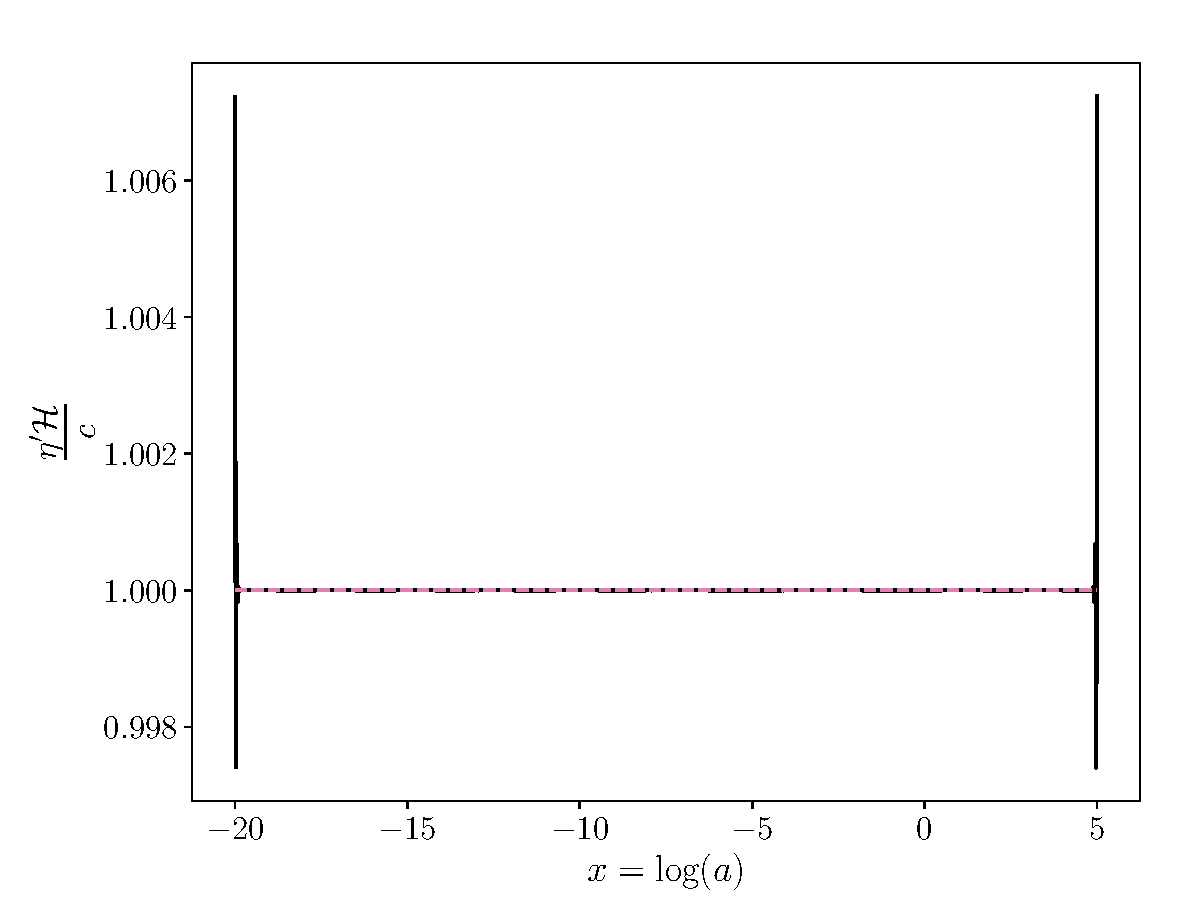
\includegraphics[width=\columnwidth]{/Users/paljettrosa/Documents/GitHub/AST5220/figs/numerical_stability.pdf}
    \caption{Comparison of the numerically computed conformal time derivative  $\eta'\mathcal{H}/c$ with the expected value of 1 (pink line). The small deviations on the order of $\lesssim 10^{-5}$ confirm the numerical stability of the integration.}\label{fig:numerical stability}
\end{figure}

To test the stability of the numerical solutions presented in the following section, I have plotted $\eta'\mathcal{H}/c$ as function of $x$ in figure \ref{fig:numerical stability}, since this quantity should remain close to unity throughout the range. The scatter points, which were obtained by taking the derivative of the spline for $\eta$, show small deviations from 1, on the order of $\lesssim 10^{-5}$, indicating that the numerical error is very small. It also remains bounded bounded throughout the range of $x$, suggesting that the ODE solver maintains stability and does not accumulate significant numerical drift. The slight periodic variations could result from finite step sizes in the integration, or have something to do with interpolation errors between the integration points, but they are well within an acceptable tolerance.

\colorbox{Plum}{TODO: maybe move over prev. sec.}


\subsection{Results and discussions}\label{subsec: I results}

\subsubsection{The conformal Hubble parameter}
\begin{figure}
  \centering
  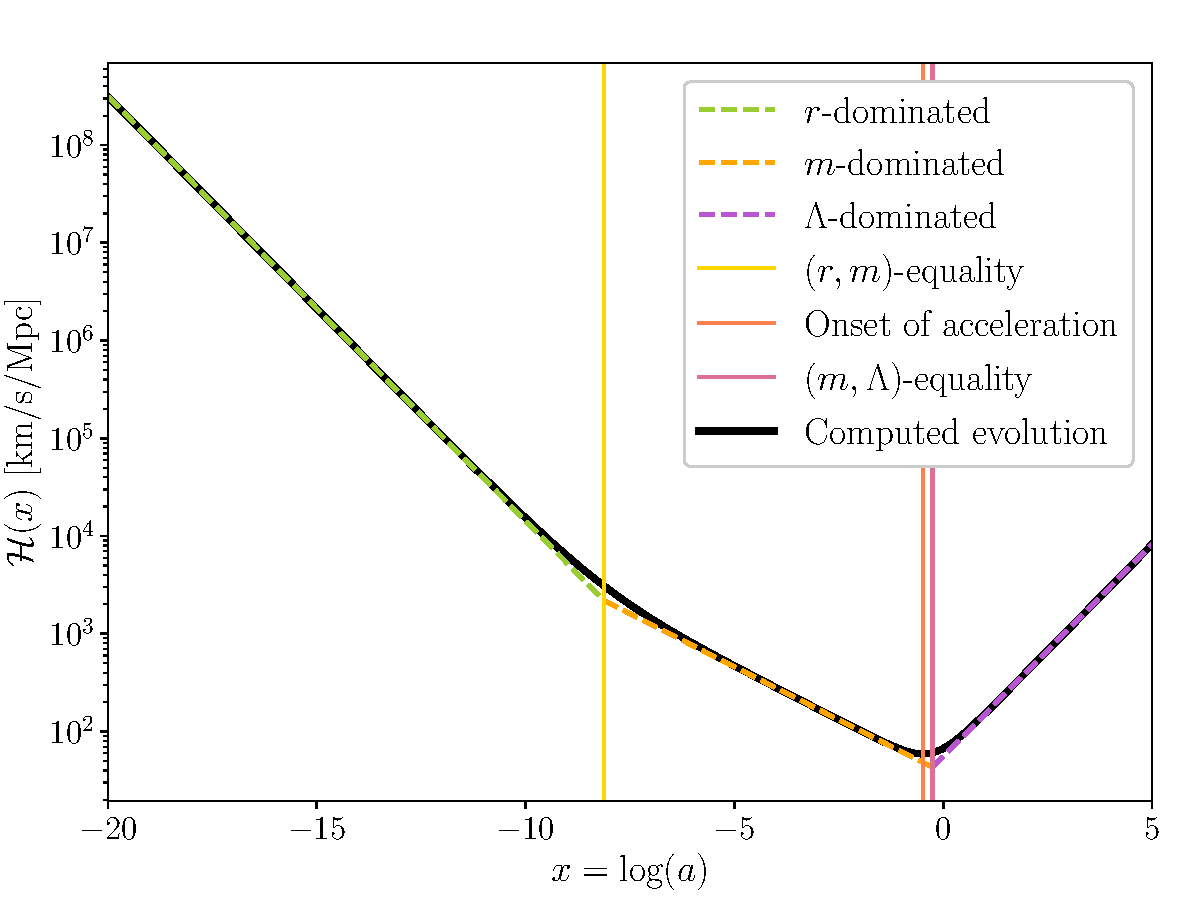
\includegraphics[width=\columnwidth]{/Users/paljettrosa/Documents/GitHub/AST5220/figs/H_prime.pdf}
  \caption{Exact evolution of the conformal Hubble parameter $\mathcal{H}(x)$ (black) compared with approximations (dashed). The onset of acceleration is visible as a departure from matter-like scaling, occuring at the trough of the exact solution.}\label{fig:H_prime}
\end{figure}


In figure \ref{fig:H_prime} I have plotted the exact evolution of the conformal Hubble parameter $\mathcal{H}(x)$ (black solid line), with approximations in the different cosmological epochs overplotted (dashed lines). Green, orange and purple correspond to radiation-, matter- and dark energy-dominated eras, respectively, with the yellow, red and pink vertical lines marking radiation-matter equality, onset of acceleration, and matter-dark energy equality. We see that the approximations closely follow the exact solution, staying at the correct order of magnitude at all times, although the deviations are significant close to the equality times. These are of course to be expected, since the approximations were derived under the assumption of the Universe only containing the dominating component within the different eras, which of course is not realistic as we transition from one to another. Thus, the result is still a great validation for the approximations, which indicates that we can safely use them to verify the numerical solutions for $\eta$ and $t$.

\begin{figure*}
    \centering
    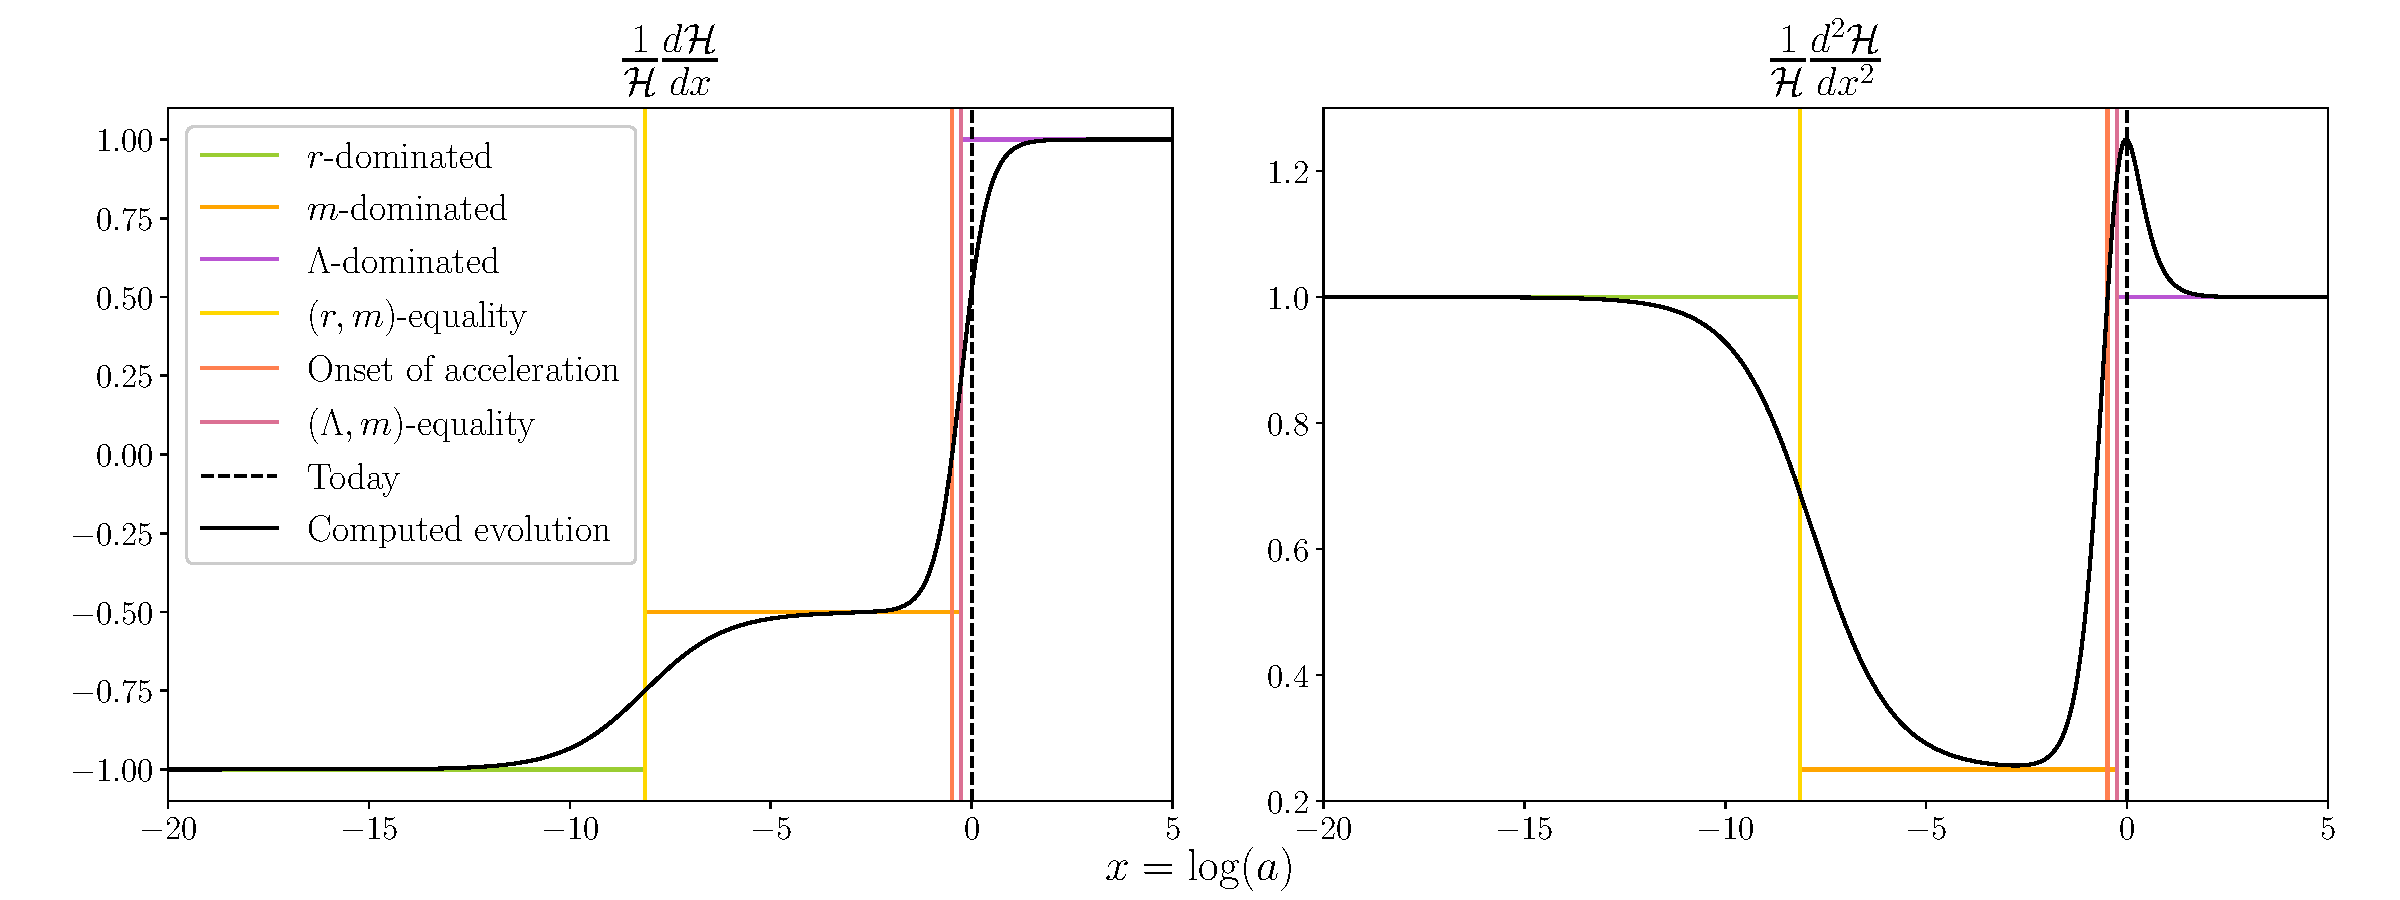
\includegraphics[width=\textwidth]{/Users/paljettrosa/Documents/GitHub/AST5220/figs/H_prime_derivatives.pdf}
    \caption{Comparison of exact evolutions (black) with approximations (dashed) for the scaled first and second derivatives of $\mathcal{H}(x)$. Agreement is good in pure radiation and matter domination but deviates near transitions due to neglected components.}\label{fig:H_prime derivatives}
\end{figure*}

A more direct comparison between the approximations and the exact evolution can be seen in figure \ref{fig:H_prime derivatives}, where I have plotted the first (left) and second (right) derivatives of $\mathcal{H}$ with respect to $x$, divided by $\mathcal{H}$ to see relative differences more easily. The dashed lines of different colors represent the same things here as well. We see good agreement in the asymptotically radiation-dominated and dark energy-dominated regimes, while in the matter-dominated epoch and around the equality times there are clear deviations, especially for the double derivative. This is reasonable, as we make rough approximations in both the beginning and the end of this era, hence the exact solution barely has time to sink to the expected value before it rises at the next transition point. 

It is interesting to see that the scaled double derivative actually increases beyond the expected value in the beginning of the dark energy-dominated era, with the peak being today. To understand this, we can look back at eqs. \eqref{eq:dHpdx} and \eqref{eq:ddHpddx}. The latter shows that the second derivative is influenced by a competition between growing and decaying terms as the Universe evolves: During the matter-dominated era, the dominant term is $\Omega_{m0} e^{-x}$, which leads to a slow decrease in $\mathcal{H}$; as $\Lambda$ begins to dominate, the exponential growth of the $2\Omega_{\Lambda 0} e^{2x}$ term starts accelerating the Universe. The transition is not instantaneous, meaning there is a period where the competing effects of matter dilution ($e^{-x}$) and dark energy growth ($e^{2x}$) cause a rapid shift in dynamics. This is visible in the sharp turn of $\mathcal{H}$ in figure \ref{fig:H_prime}, and explains the peak in the scaled second derivative before it settles into the $\Lambda$-dominated regime.


\subsubsection{Time and horizon measures}
\begin{figure*}
  \centering
  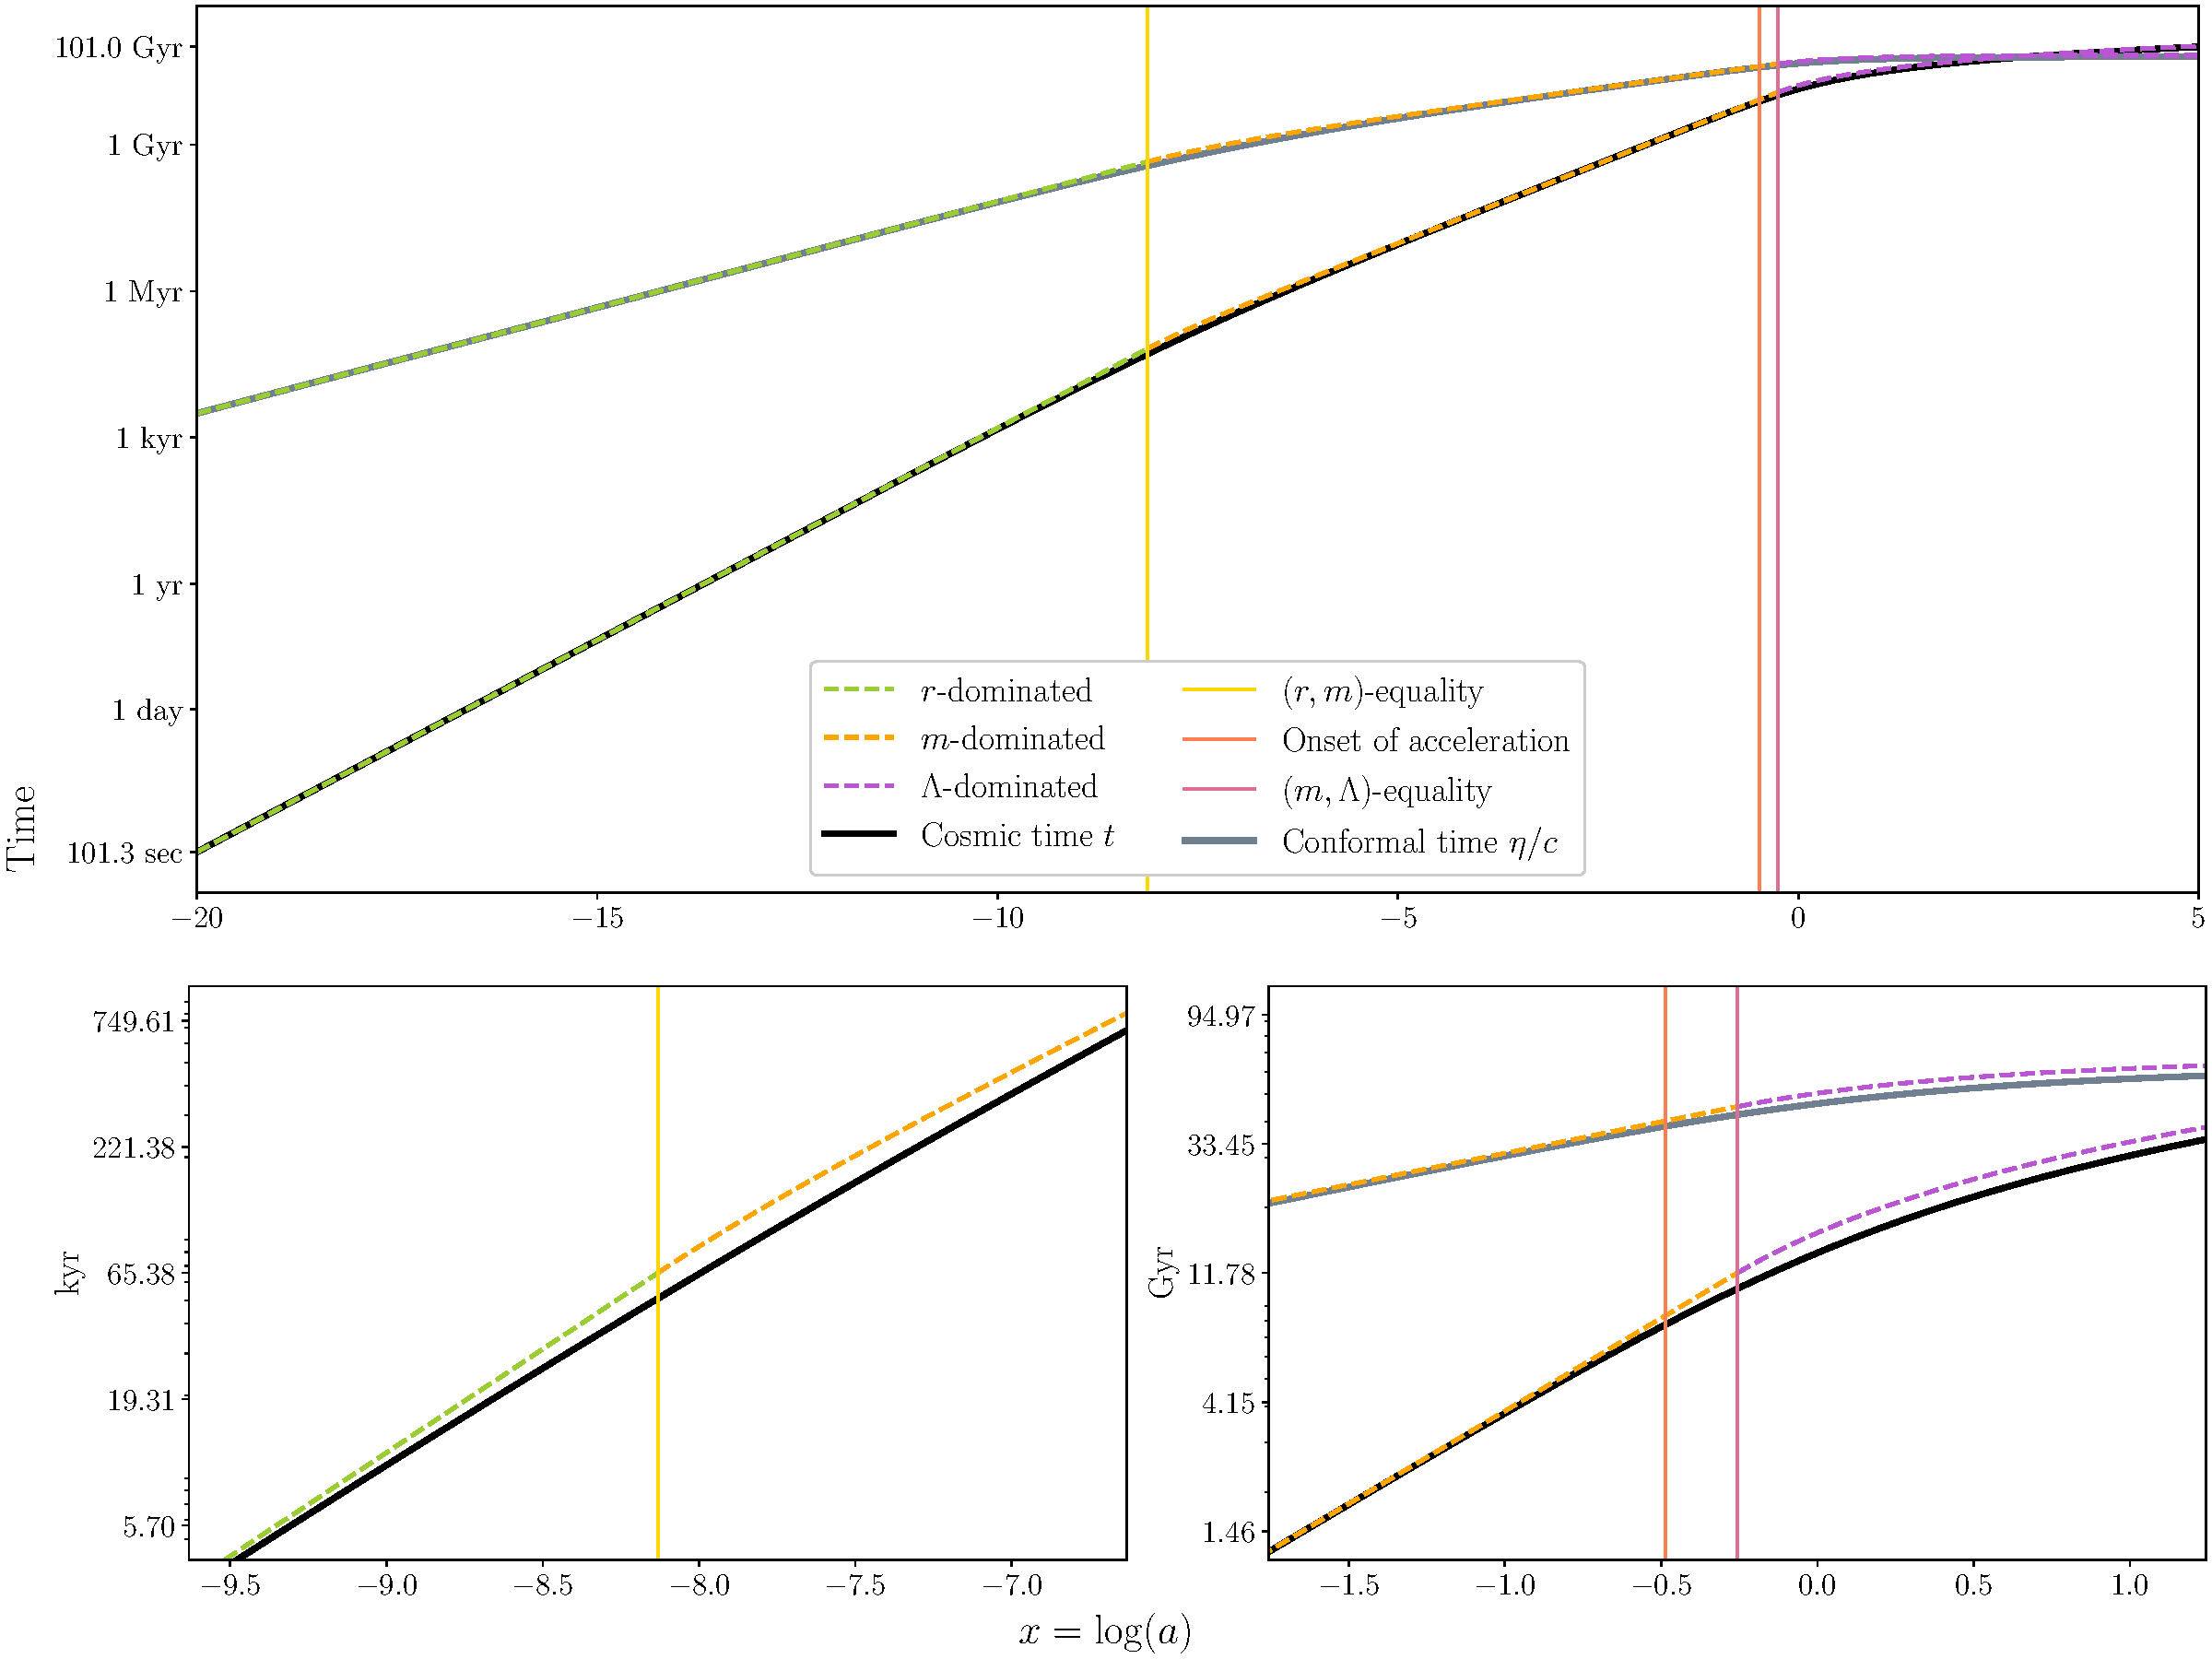
\includegraphics[width=\textwidth]{/Users/paljettrosa/Documents/GitHub/AST5220/figs/eta_and_t.pdf}
  \caption{Conformal time $\eta(x)$ (grey) and cosmic time $t(x)$ (black) compared with analytical approximations (dashed). Deviations near equality points arise due to gradual transitions between dominant energy components. This is highlighted in the bottom subplots for the cosmic time.}\label{fig:eta and t}
\end{figure*}

In figure \ref{fig:eta and t} I have plotted the numerical solutions for the conformal time $\eta/c$ (grey) and the cosmic time $t$ (black) as functions of $x$, with the approximate analytical solutions presented in section \ref{subsec: I theory} overplotted with dashed lines. The two bottom subplots, where the cosmic time is in focus, are included to easily be able to study what happens where the discrepancies between the numerical and analytical solutions are most drastic: where the Universe transitions from being dominated by one component to another. As expected, we see that the analytical approximation starts to deviate from the numerical curve as we approach $(r,m)$-equality, and eventually meets it again after. This happens also for the $(m,\Lambda)$-equality, but here the deviation actually continues to grow before it falls down again.


\begin{table*}
  \caption{Key cosmological timestamps at radiation-matter equality, the onset of acceleration, matter-dark energy equality, and present-day values. The analytical values are obtained using approximations from the theory section, while the numerical values are extracted from splines after solving the full system of equations. Discrepancies between the two highlight the limitations of the analytical approximations, especially during transition epochs.}             % title of Table
  \label{table:time stamps}      % is used to refer this table in the text
  \centering                          % used for centering table
  \begin{tabular}{| c || c | c | c | c |}        % centered columns (4 columns)
  \hline                % inserts double horizontal lines
   & Radiation-matter equality & Onset of acceleration & Matter-dark energy equality & Present day values \\    % table heading 
  \hline\hline                        % inserts single horizontal line
  \hspace{6pt}$x$\hspace{53pt} & \hspace{8.5pt}$-8.13$ & $-0.49$ & $-0.26$ & 0 \\      % inserting body of the table
  \hline 
  \hspace{6pt}$z$\hspace{53pt} & $3400.33$ & \hspace{6.5pt}$0.63$ & \hspace{7pt}$0.29$  & 0 \\
  \hline 
  \hspace{6pt}$t$ \hspace{5pt}(analytical) & \hspace{25pt}$65.38\,$kyr & \hspace{24.5pt}$8.33\,$Gyr & \hspace{19pt}$11.78\,$Gyr & \hspace{25pt}$16.30\,$Gyr \\
  \hspace{6pt}$t$ \hspace{5pt}(numerical) & \hspace{25pt}$51.06\,$kyr & \hspace{24.5pt}$7.75\,$Gyr & \hspace{19pt}$10.38\,$Gyr & \hspace{25pt}$13.86\,$Gyr \\
  \hline 
     $\eta/c$ (analytical) & \hspace{25pt}$444.75\,$Myr & \hspace{20.5pt}$40.22\,$Gyr & \hspace{19pt}$45.20\,$Gyr & \hspace{25pt}$50.36\,$Gyr \\ 
     $\eta/c$ (numerical) & \hspace{25pt}$368.44\,$Myr & \hspace{20.5pt}$38.57\,$Gyr & \hspace{19pt}$42.37\,$Gyr & \hspace{25pt}$46.32\,$Gyr \\ 
     \hline 
     \hspace{5.5pt}$\eta$ \hspace{3.5pt}(analytical) & \hspace{25pt}$136.27\,$Mpc & \hspace{20.5pt}$12.32\,$Gpc & \hspace{19pt}$13.85\,$Gpc & \hspace{25pt}$15.43\,$Gpc \\ 
     \hspace{5.5pt}$\eta$ \hspace{3.5pt}(numerical) & \hspace{25pt}$112.89\,$Mpc & \hspace{20.5pt}$11.82\,$Gpc & \hspace{19pt}$12.98\,$Gpc & \hspace{25pt}$14.19\,$Gpc \\ 
  \hline                                   %inserts single line
  \end{tabular}
  \end{table*}

In table \ref{table:time stamps} I have listed key cosmological timestamps for important transition points in the Universe's history: radiation-matter equality, the onset of acceleration, matter-dark energy equality, and present-day values. The logarithmic scale factor $x = \log a$ and redshift $z$ are listed for each event, along with analytical and numerical results for cosmic time $t$, conformal time $\eta/c$, and the comoving horizon $\eta$. We observe a discrepancy between the analytically approximated values for $t$ and $\eta$ obtained using the expressions derived in section \ref{subsec: I theory} and the corresponding numerical values, which instead were obtained by solving the full system of equations and interpolating via splines. These discrepancies are consistent with figure \ref{fig:eta and t}.

In \citet{Planck}, one presented estimate of the age of the Universe is $t_0=13.801\pm0.024\,\text{Gyr}$. This is based on $1\sigma$ constraints on a combination of gravitational lensing and TT (temperature), TE (temperature-E mode polarization), EE (E mode polarization) and lowE (low multipole E-mode polarization) angular power spectra measurements. This is in good agreement with the numerical result, although the value stated here is slightly larger. Nevertheless, the analytical approximation greatly overestimate it in comparison. This further validates the numerical solution around the equality times, where it deviates from the approximate evolutions and we have less to compare it to.

\subsubsection{Density parameters}
\begin{figure}
    \centering
    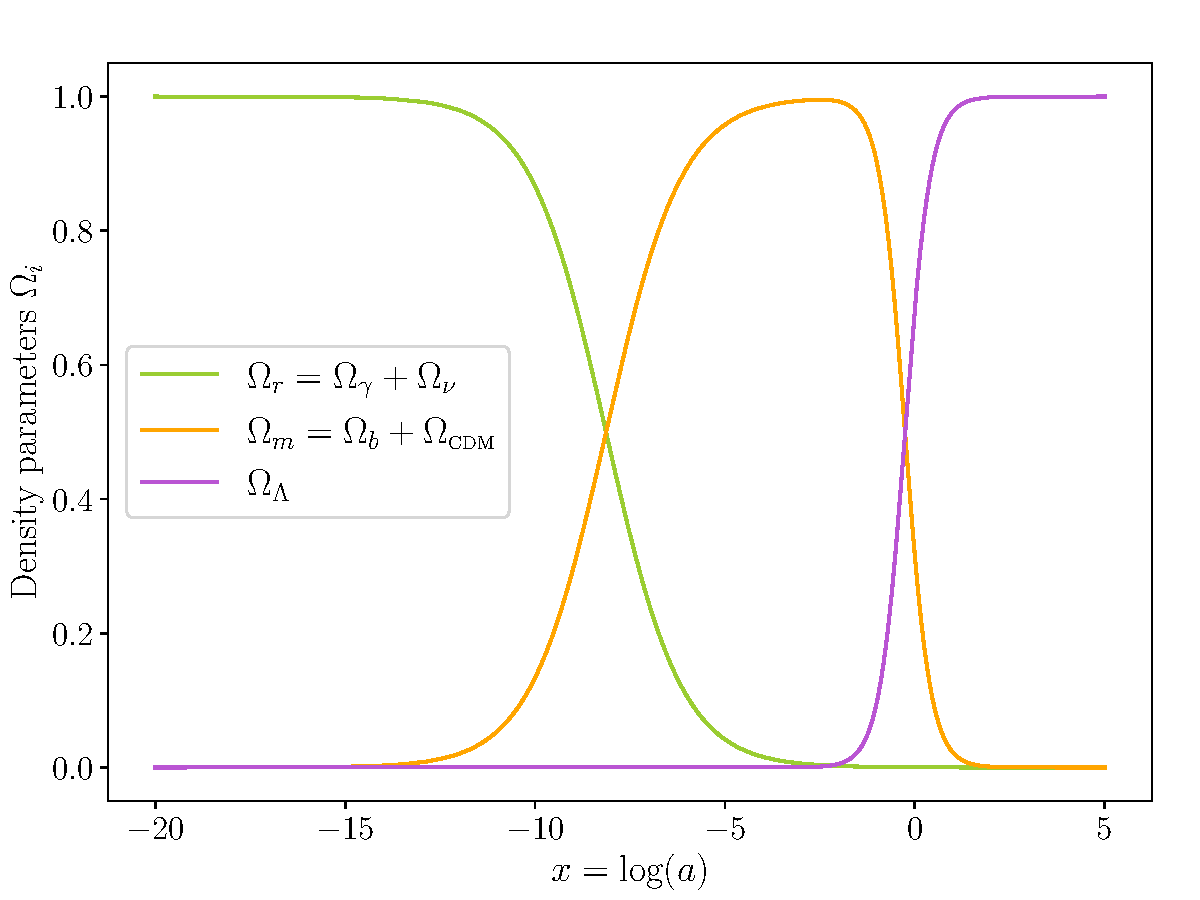
\includegraphics[width=\columnwidth]{/Users/paljettrosa/Documents/GitHub/AST5220/figs/density_parameters.pdf}
    \caption{The fractional energy densities of radiation, matter, and dark energy as functions of $x$ (solid lines). The dashed lines show the evolutions of the radiation components (photons and neutrinos) and matter components (baryons and dark matter).}\label{fig:density parameters}
\end{figure}

The evolutions of the density parameters $\Omega_i(x)$ are plotted in figure \ref{fig:density parameters}, with solid lines for $\Omega_r$, $\Omega_m$ and $\Omega_\Lambda$, and dashed lines for the individual components that make up the two first of these. The solid curves are consistent with the previous results, with the transitions between the different eras matching the observed changes in $\mathcal{H}$, $\eta$ and $t$. For example, the abrupt change in the conformal Hubble parameter at $(m,\Lambda)$-equality compared to the change at $(r,m)$-equality matches the relatively rapid takeover of $\Lambda$ as the dominating energy component, as opposed to the more gradual change from radiation to matter domination. 

\subsubsection{Supernova fitting}
% \begin{table}
%   \caption{Best-fit cosmological parameters obtained from supernova data, along with their mean values and standard deviations. The best-fit values correspond to the minimum $\chi^2$, while the Planck 2018 values are provided for comparison. The Hubble constant $H_0$ is given in units of km/s/Mpc.}             % title of Table
%   \label{table:supernova}      % is used to refer this table in the text
%   \centering                          % used for centering table
%   \begin{tabular}{| c || c | c | c | c |}        % centered columns (4 columns)
%   \hline                % inserts double horizontal lines
%    & \hspace{5pt}$\mu_i$\hspace{5pt} & \hspace{7pt}$\sigma_i$\hspace{7pt} & min$\big(\chi^2\big)$ & Planck \\    % table heading 
%   \hline\hline                     % inserts single horizontal line
%   $H_0$ & \hspace{-10pt}70.1 & \hspace{-10pt}0.5 & \hspace{-10pt}70.2 & \hspace{-10pt}67.0 \\
%   \hline
%   $\Omega_{m0}$ & \hspace{5pt}0.240 & 0.087 & \hspace{5pt}0.258 & \hspace{5pt}0.317 \\
%   \hline
%   $\Omega_{k0}$ & \hspace{5pt}0.118 & 0.216 & \hspace{5pt}0.071 & \hspace{5pt}0.000 \\
%   \hline
%   $\Omega_{\Lambda0}$ & \hspace{5pt}0.642 & 0.133 & \hspace{5pt}0.672 & \hspace{5pt}0.683 \\
%   \hline                                   %inserts single line
%   \end{tabular}
% \end{table}

\begin{table}
  \caption{Best-fit cosmological parameters obtained from supernova data, along with their mean values and standard deviations. The best-fit values correspond to the minimum $\chi^2$, while the Planck 2018 values estimated from 1$\sigma$ constraints on TT,TE,EE+lowE+lensing measurements are provided for comparison. These were determined by assuming a perfectly flat Universe, though they do actually estimate a small non-zero curvature density ($\Omega_{k0}=0.0007\pm0.0019$) when relaxing this assumption and also including BAO measurements. I have chosen to neglect this in my analysis, due to the relatively small value and large uncertainty. \colorbox{Plum}{move to main text?} Moreover, the Hubble constant is given in units of km/s/Mpc.}             % title of Table
  \label{table:supernova}      % is used to refer this table in the text
  \centering                          % used for centering table
  \begin{tabular}{| c || c | c | c | c |}        % centered columns (4 columns)
  \hline                % inserts double horizontal lines
   & \hspace{5pt}$\mu_i$\hspace{5pt} & \hspace{7pt}$\sigma_i$\hspace{7pt} & min$\big(\chi^2\big)$ & Planck \\    % table heading 
  \hline\hline                     % inserts single horizontal line
  $H_0$ & \hspace{-10pt}70.1 & \hspace{-10.2pt}0.5 & \hspace{-10.8pt}70.2 & \hspace{-5.5pt}$67.4\pm0.5$ \\
  \hline
  $\Omega_{m0}$ & \hspace{4.8pt}0.240 & \hspace{-0.2pt}0.087 & \hspace{4.6pt}0.258 & $0.315\pm0.007$ \\
  \hline
  $\Omega_{k0}$ & \hspace{0pt}0.12 & \hspace{-5pt}0.22 & \hspace{0pt}0.07 & 0 \\
  \hline
  $\Omega_{\Lambda0}$ & \hspace{5pt}0.642 & 0.133 & \hspace{5pt}0.672 & $0.685\pm0.007$ \\
  \hline                                   %inserts single line
  \end{tabular}
\end{table}


When running the MCMC fits, the minimum chi-squared value obtained was $\chi^2_\text{min}=29.2867$, corresponding to the parameter values listed in the third column of table \ref{table:supernova}. The means $\mu_i$ and standard deviations $\sigma_i$ (where $i$ runs over the parameters) computed for the samples within the $1\sigma$ constraints are listed as well, in addition to the Planck parameters stated in \cite{Planck} for comparison. Interestingly, the supernova measurements favor a slightly open universe, deviating from the Planck result of a flat universe. However, the standard deviation, which is about three times larger than the best-fit value, suggests that the data does not strongly constrain curvature. We also see that the Planck result for $\Omega_{m0}$ is higher than the best-fit value, though it is within the $1\sigma_m$ confidence interval. 
% Nevertheless, this suggests that the supernova data prefers a lower matter density, which is consistent with the higher inferred value of $H_0$. 
% Lastly, the Planck value for $\Omega_{\Lambda0}$ is only slightly larger than the best-fit value, and it is well within $1\sigma_\Lambda$. \colorbox{Plum}{correct to say this?}.

\begin{figure}
    \centering
    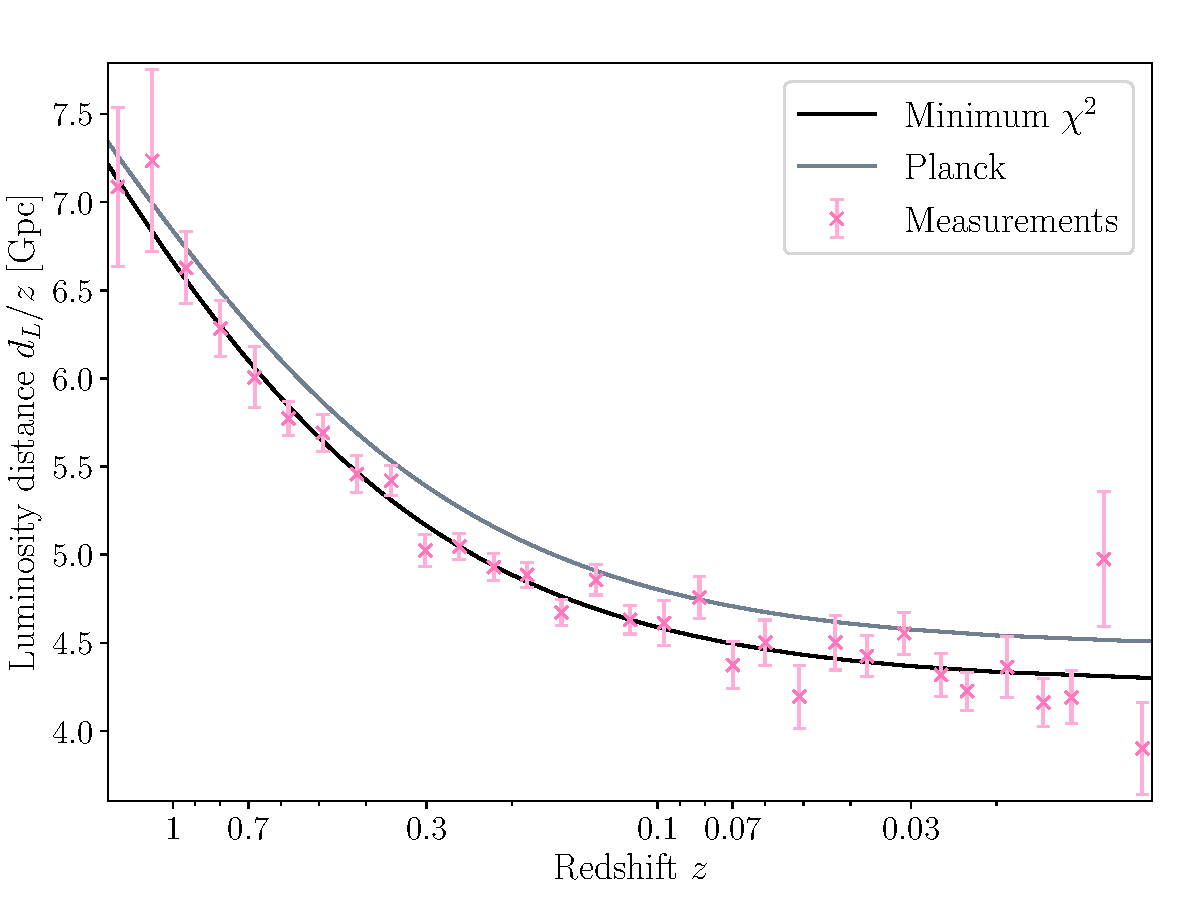
\includegraphics[width=\columnwidth]{/Users/paljettrosa/Documents/GitHub/AST5220/figs/luminosity_distance.pdf}
    \caption{Comparison of the luminosity distances $d_L^\text{obs}/z$ gathered from supernova observations (pink with errorbars) with the fiducial Planck model (grey) and the best-fit model from MCMC analysis (black).}\label{fig:luminosity distance}
\end{figure}

After obtaining the best-fit values I made a new instance of \verb|BackgroundCosmology| with these parameters and solved for this universe as well. In figure \ref{fig:luminosity distance} I have plotted the scaled luminosity distance $d_L/z$ against $z$ for this best-fit cosmology (black curve) as well as the Planck cosmology (grey curve), together with the data points $d_L^\text{obs}/z$ with scaled errorbars (pink). We see that the best-fit cosmology aligns much better with the data points than the Planck model, as the latter does not always lie within the supernova errorbars. This reflects the fact that the Planck data prefers a flat universe, whereas the best-fit suggests slightly negative curvature, which alters the distance-redshift relation. It also highlights tensions between low-redshift and high-redshift cosmological probes (see e.g. \cite{JWST} for a recent discussion of this so-called Hubble tension in light of JWST observations). However, it should be kept in mind that measurements of supernova magnitudes can be affected by calibration uncertainties, host galaxy effects and dust extinction, potentially shifting best-fit cosmological parameters. Nevertheless, the discrepancies underscore the importance of using multiple probes and datasets to break parameter degeneracies and obtain a more complete picture of cosmic expansion.


\begin{figure}
    \centering
    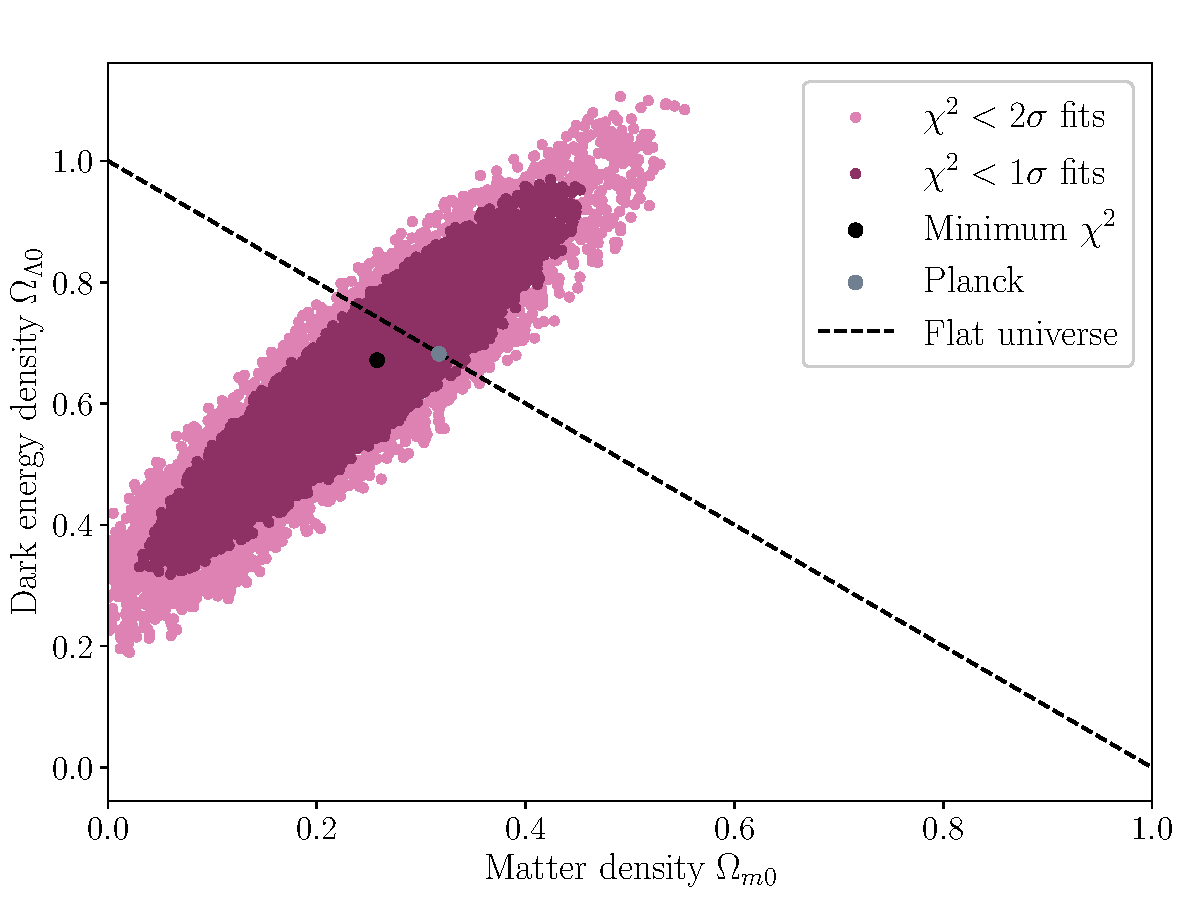
\includegraphics[width=\columnwidth]{/Users/paljettrosa/Documents/GitHub/AST5220/figs/MCMC_fits.pdf}
    \caption{Confidence contours in the $(\Omega_{m0},\Omega_{\Lambda0})$ parameter space from the supernova MCMC analysis, compared to the Planck fiducial model. The supernova constraints allow for a slightly open universe, while Planck favors flatness based on multi-probe data.}\label{fig:MCMC fits}
\end{figure}

In figure \ref{fig:MCMC fits} I have scatter plotted the accepted $(\Omega_{m0},\Omega_{\Lambda0})$ samples within the $1\sigma$ and $2\sigma$ constraints, with the black (grey) data point showing the best-fit (Planck) parameter set, and the dashed line showing the combinations that allow for a flat universe. We see clearly here that supernova-only constraints allow for slightly different cosmologies than the Planck model, with a preference for a lower matter density and small negative curvature. The Planck data includes additional information from the early universe, leading to a tighter preference for a flat universe with more mass. This discrepancy ties directly to the luminosity distance plot, confirming that these best-fit supernova parameters slightly differ from Planck's and further highlighting the importance of combining multiple datasets for robust cosmological constraints.


% When running the MCMC fits, the minimum chi-squared value obtained was $\chi^2_\text{min}=29.2867$, corresponding to the parameter values listed in the third column of table \ref{table:supernova}. The means $\mu_i$ and standard deviations $\sigma_i$ (where $i$ runs over the parameters) computed for the samples within the $1\sigma$ constraints are listed as well, in addition to the Planck parameters for comparison. We see that the best-fit value of $H_0$ based on the supernova data alone was $70.204\,$km/s/Mpc, slightly higher than the Planck result of $67\,$km/s/Mpc. This is expected, as supernova data alone tends to favor a higher $H_0$ than CMB-based analyses, a discrepancy known as the Hubble tension. We also see that the Planck result is larger than the best-fit value for $\Omega_{m0}$, though it is within $1\sigma_m$ \colorbox{Plum}{correct to say this?}. Nevertheless, this suggests that the supernova data prefers a lower matter density, which is consistent with the higher inferred value of $H_0$.

% Interestingly, the results favor a slightly open universe, deviating from the Planck result of a flat universe. However, the standard deviation, which is about three times larger than the best-fit value, suggests that the data does not strongly constrain curvature. Lastly, the Planck value for $\Omega_{\Lambda0}$ is only slightly larger than the best-fit value, and it is well within $1\sigma_\Lambda$. \colorbox{Plum}{correct to say this?}. These results highlight the differences between constraints obtained from supernova data alone versus those obtained from CMB measurements. The larger uncertainties in our fits, particularly for $\Omega_{k0}$, emphasize the need to incorporate additional cosmological probes, such as baryon acoustic oscillations (BAO) and CMB data, for tighter constraints.

\begin{figure*}
  \centering
  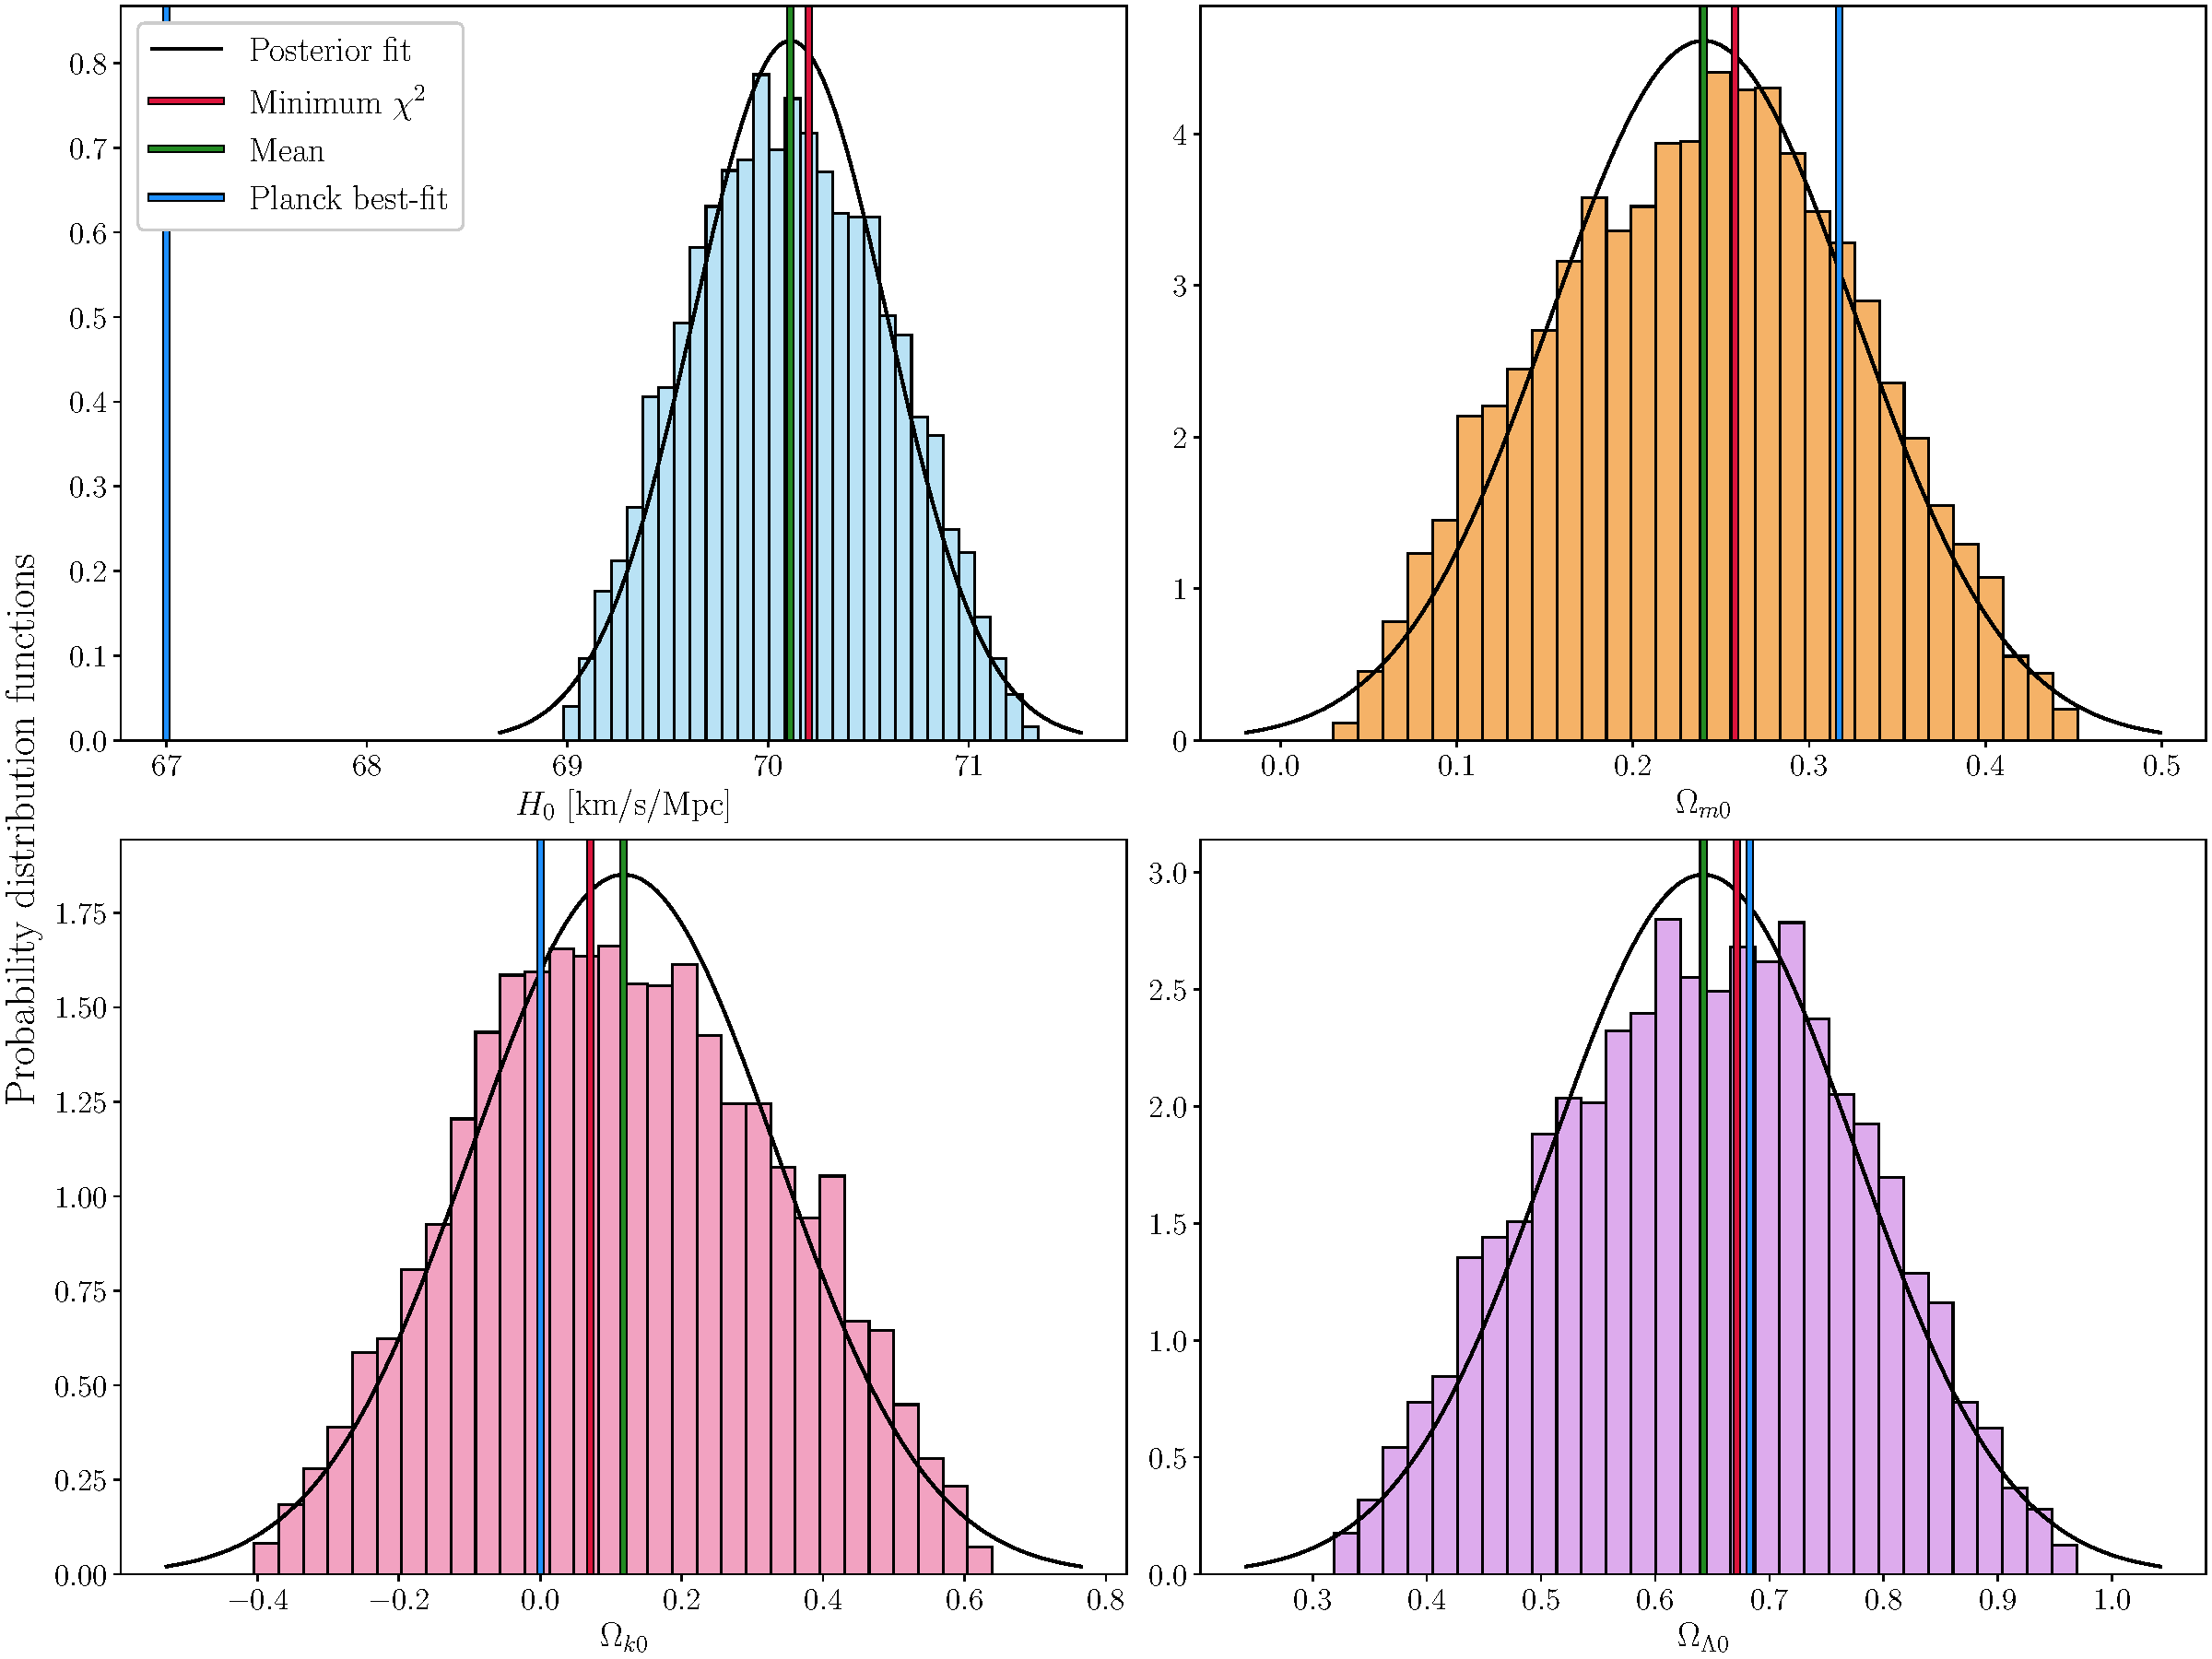
\includegraphics[width=\textwidth]{/Users/paljettrosa/Documents/GitHub/AST5220/figs/distributions.pdf}
  \caption{Histograms of the MCMC posterior distributions for the parameters $(H_0,\Omega_{m0}, \Omega_{k0}, \Omega_{\Lambda0})$, compared with Gaussian fits (solid curves) and Planck values. Deviations from Gaussianity indicate asymmetries in parameter uncertainties. \colorbox{Plum}{TODO: maybe change lines}}\label{fig:distributions}
\end{figure*}

Figure \ref{fig:distributions} shows normalized histograms of the samples within the 1$\sigma$ constraint, with Gaussian fits made with the $\mu_i$ and $\sigma_i$ overplotted to represent the posterior distributions. Most noticeable is how different the supernova and Planck results are for $H_0$, with the smallest accepted $1\sigma$ samples being as large as $69\,$km/s/Mpc. Planck's estimate is derived from early universe physics (CMB, baryon acoustic oscillations and large-scale structure), while supernova constraints come from low-redshift expansion. The discrepancy may therefore indicate new and/or unknown physics present at some eras of the expansion history (see \cite{JWST}, but also \cite{tensions} for critical discussions on tensions as indicators of new physics), or possibly systematic errors in one or both datasets. Moreover, we see that the supernova-only constraint clearly prefers a lower matter density compared than the Planck estimate, consistent with the MCMC contour plot.

The posterior distribution suggests a preference for a slightly open universe, though with considerable uncertainty. This deviation from flatness may arise because supernovae alone do not tightly constrain curvature, as they primarily measure relative distances, not absolute spatial curvature. Moreover, we see that the histograms are not perfectly Gaussian, particularly those for $\Omega_{m0}$ and $\Omega_{k0}$. Specifically, the asymmetry with more samples in the low mass/negative curvature ends may suggest a skewed uncertainty, indicating that a simple Gaussian error estimate might underestimate the possible range of accepted values. 

\colorbox{Plum}{maybe remove/argue for good in ast. standards}
% Alarmingly, the $H_0$ distribution appears more symmetric, indicating that supernova data alone provide a more stable estimate for the Hubble constant, which deviates the most from the Planck result.




\section{Milestone II: Recombination History}\label{sec: milestone II}
In the previous milestone, I established a numerical framework for solving the background evolution of the Universe, validating the results against analytical approximations and observational constraints. This provided a foundation for understanding the expansion history and cosmic distances, key ingredients in interpreting cosmological data. However, to model the formation of the CMB and its anisotropies, we must now extend the analysis to include recombination history: the period when the Universe transitioned from an ionized plasma to a neutral state, allowing photons to decouple from matter. This process determines the surface of last scattering, setting the initial conditions for the CMB fluctuations we observe today.  

In this milestone, I compute the recombination and reionization history by solving the Saha and Peebles equations, track the evolution of the optical depth $\tau(x)$, and derive the visibility function $\tilde{g}(x)$, which quantifies when CMB photons last interacted with free electrons. These quantities are essential for accurately modeling the temperature and polarization anisotropies of the CMB in the next milestones. Additionally, I compute the sound horizon at decoupling, a fundamental scale imprinted in the CMB power spectrum. This milestone bridges the gap between background cosmology and perturbation theory, ensuring that my model of the early Universe correctly captures the physics governing photon-matter interactions before recombination. \colorbox{Plum}{maybe change/shorten}


\subsection{Theoretical framework}\label{subsec: II theory}
\begin{enumerate}
  \item [1.] Write out the distribution function $f$ for fermions and bosons, and show that it reduces to the Maxwell-Boltzmann distribution in the low energy limit.
  \item [2.] State the Boltzmann equation in general relativity, written in terms of an affine parameter $\lambda$, the time $t$, the spatial components $x^i$, the energy $E$, the zero'th component of the four-momentum $P^0$, and the unit three-momentum vector $\hat{p}^i$. Explain that we use the unit vector since it vanishes in linear perturbation theory? Define also the moments of the Boltzmann equation (number density, energy density apnd pressure).
  \item [3.] Explain what the collision term is, and that we will simply use results from quantum field theory calculations. Explain that it is zero in a smooth universe where the particles are in equilibrium with the thermal bath.
  \item [4.] Explain that we usually consider $1+2\leftrightarrow3+4$ processes in cosmology, such as electron-positron annihilation and pair production, Compton (Thompson i low energy limit?) and Coulomb scattering, and hydrogen recombination / ionization. Write out these interaction processes. 
  \item [5.] Explain which interaction is relevant at this point in time and for the CMB: Compton scattering in the low energy limit (Thompson scattering), and explain why this is the most important.
  \item [6.] Write out the Boltzmann equation for such a process in a smooth universe, and explain what the parameters $\alpha$ and $\beta$ are. Explain that $\beta$ is defined in terms of $\alpha$ and the equilibrium number density values.
  \item [7.] Explain what decoupling and freeze-out is, and define these limits in terms of the Boltzmann equation. Explain why it is crucial for our purposes.
  \item [8.] Explain that it is hard to know exact number densities and that we instead use the fraction parameters. Define these and state all the fraction parameters (free electron fraction $X_e$, primordial Helium fraction $Y_p$, as well as $x_\text{He++}$, $x_\text{He+}$ and $x_\text{H+}$).
  \item [9.] Derive the Saha approximation, and state the Saha equations when including Helium.
  \item [10.] Move on to explain that we need the Peebles equation when the free electron fraction $X_e<0.99$, and state this. State also all of the atomic physics constants. Make sure to include Helium.
  \item [11.] Explain how we can improve the results by including the fudge factor $f$ to the Peebles equation, and reference Recfast.
  \item [12.] Define the optical depth, and explain that this is a crucial quantity that we need to have a firm grasp on. Derive its first and second derivatives with respect to $x$, and explain why we must integrate it in the same way as we did for $\eta$ and $t$, but starting from today's value.
  \item [13.] Define the visibility function and explain its importance, and what it represents. Derive its first and second derivatives with respect to $x$.
  \item [14.] Define the optical depth for baryons, and explain why it is important to include it for accuracy. Explain what the baryon drag epoch is.
  \item [15.] Explain that a typical approximation to make is to set the baryon temperature equal to the photon temperature at all times, but that it is necessary to include it for full accuracy. Derive the baryon temperature equation from the Boltzmann equation, and compare it to the photon temperature equation.
  \item [16.] Define the sound horizon, and explain why we need to know it at decoupling, and why it will be interesting to know it at the drag epoch.
  \item [17.] Explain what reionization is, why it happened and why we should include it for accurate results. State the relevant equations, and explain that we must ``turn it off'' when computing certain quantities, such as the freeze-out abundance of free electrons today.
\end{enumerate}

% Point 1 is for subsection 1, points 2-7 for subsection 2, point 8 for subsection 3, 9 for subsection 4, 10 and 11 for subsection 5, 12-14 for subsection 6, 15 for subsection 7, 16 for subsection 8, and point 17 for subsection 9. 

% Can you write subsection 8 about sound horizons? Make sure to include point 16. Be concise and thorough, and match my writing style from the previous milestone.




\subsubsection{Distribution functions}
\color{Plum}
In cosmology, the evolution of particle species is governed by their phase-space distribution function, $f$, which describes the number density of particles in a given region of phase space. For a system in thermal equilibrium, the distribution function is dictated by quantum statistics, specifically the Bose-Einstein and Fermi-Dirac distributions:
\begin{equation}
f_{\text{BE}}(E) = \frac{1}{e^{(E - \mu) / T} - 1}, \quad f_{\text{FD}}(E) = \frac{1}{e^{(E - \mu) / T} + 1}.
\end{equation}
Here, $E$ is the energy of the particle, $\mu$ is the chemical potential, and $T$ is the temperature of the system. The difference in the denominator arises due to quantum statistics: bosons ($f_{\text{BE}}$) obey Bose-Einstein statistics and exhibit stimulated emission, while fermions ($f_{\text{FD}}$) obey the Pauli exclusion principle, preventing multiple particles from occupying the same state.

In the limit where the thermal energy is much larger than the rest mass, $E \approx p$, and the distributions describe highly relativistic particles, such as photons and neutrinos in the early universe. However, for non-relativistic particles ($E \gg T$), the exponential terms in the denominator dominate, leading to the classical Maxwell-Boltzmann distribution:
\begin{equation}
f_{\text{MB}}(E) \approx e^{-(E - \mu) / T}.
\end{equation}
This approximation is valid for massive species that are thermally decoupled or at sufficiently low temperatures. It plays a crucial role in describing the abundance of baryons and cold dark matter in the late universe.

The phase-space distribution functions serve as the foundation for the Boltzmann equation, which governs the evolution of number densities, energy densities, and momenta of different species as the universe expands. In the following section, we introduce the Boltzmann equation in its general form, establish its key moments, and highlight its role in tracking the ionization history of the universe.
\color{black}








\subsubsection{The Boltzmann equation}
\color{Plum}
The Boltzmann equation governs the evolution of the phase-space distribution function $f$, which encapsulates the statistical properties of a given particle species in the expanding universe. It describes how the number density, energy density, and pressure of a species evolve due to the combined effects of cosmic expansion and interactions with other particles.

In general relativity, the Boltzmann equation can be written as a Liouville-type equation in terms of the affine parameter $\lambda$:
\begin{equation}
\frac{df}{d\lambda} = C[f],
\end{equation}
where $C[f]$ is the collision term, which accounts for interactions between particles. The left-hand side represents the free-streaming evolution of the distribution function, while the right-hand side encodes scattering, annihilation, and creation processes.

To express the equation in a more practical form, we rewrite it in terms of the proper time $t$, spatial position $x^i$, energy $E$, and the zero-component of the four-momentum $P^0$:
\begin{equation}
\frac{df}{dt} + \frac{dx^i}{dt} \frac{\partial f}{\partial x^i} + \frac{dE}{dt} \frac{\partial f}{\partial E} + \frac{d\hat{p}^i}{dt} \frac{\partial f}{\partial \hat{p}^i} = C[f].
\end{equation}
Here, $\hat{p}^i$ is the unit three-momentum vector, which is often used because it vanishes in linear perturbation theory, simplifying calculations when studying small fluctuations in the cosmic plasma.

Since the full distribution function is difficult to track, we instead take moments of the Boltzmann equation to extract physically relevant quantities. The number density $n$, energy density $\rho$, and pressure $P$ are given by weighted integrals over momentum space:
\begin{equation}
n = \frac{g}{(2\pi)^3} \int f d^3p, \quad
\rho = \frac{g}{(2\pi)^3} \int E f d^3p, \quad
P = \frac{g}{(2\pi)^3} \int \frac{p^2}{3E} f d^3p.
\end{equation}
Taking moments of the Boltzmann equation allows us to derive conservation equations, which describe how mass, momentum, and energy evolve over time.

 The Collision Term and Decoupling

The collision term $C[f]$ is generally obtained from quantum field theory and encodes interactions between particles. In a homogeneous and isotropic universe, it vanishes when species are in thermal equilibrium, as detailed balance ensures that the rate of interactions maintains the equilibrium distribution.

In cosmology, we primarily consider $1+2 \leftrightarrow 3+4$ interactions, such as:
\begin{enumerate}
  \item [-] Electron-positron annihilation: $e^- + e^+ \leftrightarrow \gamma + \gamma$,
  \item [-] Compton scattering: $e^- + \gamma \leftrightarrow e^- + \gamma$,
  \item [-] Coulomb scattering: $e^- + p \leftrightarrow e^- + p$,
  \item [-] Hydrogen recombination and ionization: $e^- + p \leftrightarrow \text{H} + \gamma$.
\end{enumerate}

For recombination history, the most relevant interaction is Compton scattering in its low-energy (Thomson) limit, which governs the coupling between electrons and photons before recombination.

As the universe expands and cools, interactions eventually become inefficient, leading to freeze-out or decoupling. This occurs when the interaction rate $\Gamma$ drops below the Hubble expansion rate $H$, meaning that particles can no longer maintain thermal equilibrium:
\begin{equation}
\frac{\Gamma}{H} \ll 1.
\end{equation}
This condition is crucial for understanding the transition from an ionized plasma to a neutral universe. In the next section, we introduce fraction parameters to describe the ionization state of the universe and lay the groundwork for modeling recombination.
\color{black}






\subsubsection{Mass fractions}
\color{Plum}
Instead of tracking the absolute number densities of different particle species, it is often more convenient to work with mass fractions, which describe the relative abundance of each species in a given system. This approach simplifies calculations, particularly in scenarios where the total number of particles is conserved or evolves in a predictable manner.

For recombination, we define the free electron fraction $X_e$, which quantifies the number of free electrons relative to the total number of hydrogen nuclei:
\begin{equation}
X_e = \frac{n_e}{n_H},
\end{equation}
where $n_e$ is the number density of free electrons and $n_H$ is the number density of hydrogen nuclei (both ionized and neutral).

Since helium is also present in the early universe, we define the primordial helium mass fraction $Y_p$, which represents the fraction of baryonic mass in helium:
\begin{equation}
Y_p = \frac{4 n_{\text{He}}}{n_{\text{b}}},
\end{equation}
where $n_{\text{He}}$ is the number density of helium nuclei and $n_{\text{b}}$ is the total baryon number density. The factor of 4 accounts for the fact that helium nuclei (helium-4) have four nucleons each.

To fully describe the ionization state of the universe, we also introduce the ionization fractions of hydrogen and helium:
\begin{equation}
x_{\text{H+}} = \frac{n_{\text{H}^+}}{n_H}, \quad
x_{\text{He+}} = \frac{n_{\text{He}^+}}{n_{\text{He}}}, \quad
x_{\text{He++}} = \frac{n_{\text{He}^{++}}}{n_{\text{He}}}.
\end{equation}
Here, $x_{\text{H+}}$ represents the fraction of ionized hydrogen, while $x_{\text{He+}}$ and $x_{\text{He++}}$ describe singly and doubly ionized helium, respectively.

These mass fractions allow us to track the recombination process efficiently. In the fully ionized early universe, we have $X_e \approx 1$, meaning nearly all electrons are free. As recombination progresses, electrons combine with protons and helium nuclei to form neutral atoms, reducing $X_e$ until it asymptotically approaches a small residual value due to incomplete recombination.

In the next section, we introduce the Saha approximation, which provides an analytical estimate for the free electron fraction in the early stages of recombination, before the more detailed Peebles equation is required.
\color{black}







\subsubsection{The Saha approximation}
\color{Plum}
To determine how recombination proceeds, we need to quantify the balance between ionization and recombination processes. In the early universe, interactions between photons and free electrons maintain thermal equilibrium, allowing us to approximate the electron number density using statistical mechanics. The Saha equation provides an analytical expression for this equilibrium, valid when the ionization and recombination rates are fast compared to the Hubble expansion.

The relevant interaction at this epoch is Thomson scattering, a low-energy limit of Compton scattering, which dominates the interactions between photons and free electrons. The process of hydrogen ionization and recombination can be written as:
\begin{equation}
p + e^- \leftrightarrow H + \gamma.
\end{equation}
Similarly, for helium, we include singly and doubly ionized states:
\begin{equation}
\text{He}^{++} + e^- \leftrightarrow \text{He}^+ + \gamma, \quad
\text{He}^+ + e^- \leftrightarrow \text{He} + \gamma.
\end{equation}
To determine the equilibrium abundances of free electrons, protons, and hydrogen atoms, we start from the Boltzmann equation, which describes the evolution of the distribution function of each species. However, since we assume thermal equilibrium at this stage, we can use results from statistical mechanics.

The number density $n_i$ of a species in thermal equilibrium follows from the Maxwell-Boltzmann distribution:
\begin{equation}
n_i = g_i \left( \frac{m_i k_B T}{2\pi \hbar^2} \right)^{3/2} e^{-E_i / k_B T},
\end{equation}
where $g_i$ is the statistical degeneracy factor, $m_i$ is the particle mass, $T$ is the temperature, and $E_i$ is the ionization energy.

Applying this to the ionization balance of hydrogen, we obtain the Saha equation:
\begin{equation}
\frac{n_e n_p}{n_H} = \left( \frac{m_e k_B T}{2\pi \hbar^2} \right)^{3/2} e^{-E_H / k_B T},
\end{equation}
where $E_H$ is the hydrogen ionization energy ($E_H = 13.6$ eV). This equation tells us the ratio of ionized to neutral hydrogen as a function of temperature.

Since we are interested in recombination in terms of mass fractions, we rewrite the Saha equation in terms of the free electron fraction $X_e$:
\begin{equation}
\frac{X_e^2}{1 - X_e} = \frac{1}{n_H} \left( \frac{m_e k_B T}{2\pi \hbar^2} \right)^{3/2} e^{-E_H / k_B T}.
\end{equation}
A similar expression holds for singly ionized helium:
\begin{equation}
\frac{x_{\text{He+}}^2}{1 - x_{\text{He+}}} = \frac{1}{n_{\text{He}}} \left( \frac{m_e k_B T}{2\pi \hbar^2} \right)^{3/2} e^{-E_{\text{He+}} / k_B T}.
\end{equation}
And for doubly ionized helium:
\begin{equation}
\frac{x_{\text{He++}}^2}{1 - x_{\text{He++}}} = \frac{1}{n_{\text{He}}} \left( \frac{m_e k_B T}{2\pi \hbar^2} \right)^{3/2} e^{-E_{\text{He++}} / k_B T}.
\end{equation}
These equations govern recombination at high temperatures, where thermal equilibrium holds. However, as the universe expands, the recombination rate slows relative to the expansion rate, leading to out-of-equilibrium recombination. At this point, the Saha equation no longer applies, and we must instead use the Peebles equation, which we introduce in the next section.
\color{black}
\colorbox{Plum}{fix so that first equation includes Helium}








\subsubsection{The Peebles equation}
\color{Plum}
The Saha approximation provides an accurate description of recombination in the early stages when the ionization and recombination processes are in thermal equilibrium. However, as the universe expands and cools, the recombination rate slows down relative to the Hubble expansion, preventing the free electron fraction $X_e$ from immediately following the equilibrium prediction. To accurately model recombination at later times, when $X_e < 0.99$, we must instead use the Peebles equation, which describes the evolution of $X_e$ in an out-of-equilibrium setting.

Recombination is governed by the balance between ionization and recombination processes. The rate equation for the free electron fraction $X_e$ is given by
\begin{equation}
\frac{dX_e}{dx} = \frac{C_r}{H x} \left[ \beta_H (1 - X_e) - \alpha_H n_H X_e^2 \right],
\end{equation}
where $\alpha_H$ is the hydrogen recombination coefficient, $\beta_H$ is the photoionization rate, $n_H$ is the number density of hydrogen nuclei,
and $C_r$ is the Peebles correction factor, which accounts for the fact that some recombinations result in excited hydrogen states instead of directly producing neutral hydrogen.

The Peebles correction factor is given by
\begin{equation}
C_r = \frac{\Lambda_{2s \to 1s} + \Lambda_{\alpha}}{\Lambda_{2s \to 1s} + \Lambda_{\alpha} + \beta_H},
\end{equation}
where $\Lambda_{2s \to 1s}$ is the spontaneous two-photon decay rate of the hydrogen 2s state, and $\Lambda_{\alpha}$ is the Ly-$\alpha$ escape rate, which accounts for the fact that Ly-$\alpha$ photons can redshift out of resonance before being reabsorbed.

To extend the Peebles equation to include helium recombination, we define similar equations for the helium ionization states, using analogous rate coefficients $\alpha_{\text{He+}}$ and $\alpha_{\text{He++}}$, along with their respective Peebles factors.

Additionally, empirical studies of recombination, such as those implemented in the Recfast code, introduce a fudge factor $f$ to better match the results of detailed radiative transfer simulations. The modified equation including this correction takes the form:
\begin{equation}
\frac{dX_e}{dx} = f \frac{C_r}{H x} \left[ \beta_H (1 - X_e) - \alpha_H n_H X_e^2 \right].
\end{equation}
This correction accounts for subtle radiative transfer effects and improves agreement with high-precision numerical calculations.

The Peebles equation, with its corrections for helium and additional refinements from Recfast, provides a more accurate description of recombination than the Saha equation alone. With this in place, we can now compute the free electron fraction $X_e$ throughout the recombination epoch, which will be crucial for understanding the optical depth and visibility function discussed in the next section.
\color{black}
\colorbox{Plum}{maybe derive expressions?}









\subsubsection{Optical depths and the visibility function}
\color{Plum}
To understand how photons interact with matter during recombination, we introduce the optical depth, which quantifies the probability of a photon scattering as it travels through the universe. The visibility function is then derived from the optical depth and characterizes when the last scattering of CMB photons occurred. These quantities are essential for describing how the Cosmic Microwave Background (CMB) was imprinted and later observed.

The optical depth $\tau(x)$ at a given time $x = \log a$ is defined as the integrated Thomson scattering rate along the line of sight:
\begin{equation}
\tau(x) = \int_x^0 dx' \, \sigma_T n_e c \frac{dt}{dx'},
\end{equation}
where $\sigma_T$ is the Thomson scattering cross-section and $n_e$ is the free electron number density.

Since the integral accumulates the scattering probability from the present time backward, the optical depth increases towards the past, with $\tau(x) \to 0$ today. To numerically evaluate $\tau(x)$, we solve the differential equation:
\begin{equation}
\frac{d\tau}{dx} = -\sigma_T n_e c \frac{1}{H e^x},
\end{equation}
where we integrate starting from $\tau(0) = 0$.

For later use, we also compute the second derivative, which is useful for defining the visibility function:
\begin{equation}
\frac{d^2 \tau}{dx^2} = -\frac{d}{dx} \left( \sigma_T n_e c \frac{1}{H e^x} \right).
\end{equation}
This derivative helps characterize the sharpness of the last scattering surface.

The visibility function $g(x)$ gives the probability density that a CMB photon last scattered at time $x$ and is defined as:
\begin{equation}
g(x) = -\frac{d\tau}{dx} e^{-\tau(x)}.
\end{equation}
This function peaks around the recombination epoch, when $\tau(x) \sim 1$, meaning photons were transitioning from being frequently scattered to freely propagating. The width of $g(x)$ determines how sharply defined the last scattering surface is.

To refine our understanding, we also compute the first and second derivatives:
\begin{equation}
\frac{dg}{dx} = \left( \frac{d^2\tau}{dx^2} + \left(\frac{d\tau}{dx}\right)^2 \right) e^{-\tau(x)}.
\end{equation}
These derivatives provide insight into how rapidly recombination occurred and how diffusion damping affects the CMB anisotropies.

A related quantity is the baryon optical depth, which describes the drag exerted on baryons due to interactions with photons. It is given by:
\begin{equation}
\tau_b(x) = \int_x^0 dx' \, \sigma_T n_e \frac{\rho_\gamma}{\rho_b} c \frac{dt}{dx'}.
\end{equation}
Here, the ratio $\rho_\gamma / \rho_b$ accounts for how photon pressure affects baryon motion. The epoch when $\tau_b(x) \sim 1$ defines the baryon drag epoch, which is important for understanding baryon acoustic oscillations (BAO).

The optical depth $\tau(x)$ and its derivatives define the visibility function $g(x)$, which determines the last scattering surface of the CMB. These quantities are crucial for accurately computing the anisotropies in the CMB power spectrum. Additionally, the baryon optical depth $\tau_b(x)$ helps describe the physics of BAO, connecting early universe physics to large-scale structure observations.
\color{black}
\colorbox{Plum}{do explicit calculations}








\subsubsection{The baryon temperature}
\color{Plum}
A common approximation in cosmology is to assume that the baryon temperature $T_b$ follows the photon temperature $T_\gamma$ at all times due to rapid interactions between baryons and photons. However, after recombination, when free electrons become sparse, Compton scattering becomes inefficient, and the baryon temperature evolves independently. To ensure accuracy in our computations, we must track the full evolution of $T_b$.

The baryon temperature is governed by the Boltzmann equation, which describes energy exchange between baryons and photons. In a smooth, homogeneous universe, the evolution of $T_b$ is given by:
\begin{equation}
\frac{dT_b}{dx} = -2 T_b + \frac{\Gamma_C}{H x} (T_\gamma - T_b),
\end{equation}
where $\Gamma_C$ is the Compton heating rate, given by
\begin{equation}
\Gamma_C = \frac{8 \sigma_T a_r T_\gamma^4}{3 m_e c} \frac{x_e}{1 + f_{\text{He}} + x_e}.
\end{equation}
Here, $\sigma_T$ is the Thomson cross-section, $a_r$ is the radiation constant, $m_e$ is the electron mass, and $x_e$ is the free electron fraction. The factor $f_{\text{He}}$ accounts for helium, with $f_{\text{He}} = Y_p / (4 (1 - Y_p))$, where $Y_p$ is the primordial helium fraction.

At early times, when $x_e \approx 1$, the Compton heating rate is large, keeping $T_b \approx T_\gamma$. However, after recombination, $x_e$ decreases, reducing $\Gamma_C$. Once $\Gamma_C / H \ll 1$, Compton scattering is too weak to maintain equilibrium, and the baryons thermally decouple from the photons. From this point on, $T_b$ follows the standard adiabatic evolution:
\begin{equation}
T_b \propto a^{-2}.
\end{equation}
This transition marks a key moment in the thermal history of the universe, as it affects the formation of structures and the propagation of acoustic waves in the baryon-photon fluid.

To accurately model recombination, we must compute the evolution of $T_b$ separately from $T_\gamma$. This is crucial for determining the sound speed of baryons, which in turn influences the sound horizon at recombination and the baryon acoustic oscillations (BAO). Thus, including the baryon temperature evolution is essential for precise predictions of the cosmic microwave background and large-scale structure formation.
\color{black}








\subsubsection{Sound horizons}
\color{Plum}
The sound horizon represents the maximum distance that a sound wave can propagate in the primordial plasma before recombination. It plays a crucial role in setting the scale of baryon acoustic oscillations (BAO) and determining the characteristic peaks in the cosmic microwave background (CMB) power spectrum. Accurately computing the sound horizon is essential for making precise predictions about the observed large-scale structure of the universe.

The sound horizon at a given time $t$ (or equivalently, at a scale factor $a$) is given by the integral of the sound speed $c_s$ over cosmic time:
\begin{equation}
r_s(a) = \int_0^t c_s \, dt = \int_0^a \frac{c_s}{aH} da.
\end{equation}
Here, $H$ is the Hubble parameter, and $c_s$ is the speed of sound in the tightly coupled baryon-photon plasma, given by:
\begin{equation}
c_s = \frac{1}{\sqrt{3(1 + R)}}, \quad \text{where} \quad R = \frac{3\rho_b}{4\rho_\gamma}.
\end{equation}
The parameter $R$ quantifies the relative importance of baryons compared to photons in the plasma, with $\rho_b$ and $\rho_\gamma$ being the baryon and photon energy densities, respectively. At early times, photons dominate, and $c_s \approx 1/\sqrt{3}$, but as the universe expands and baryons become more influential, $c_s$ decreases.

The sound horizon is most relevant at two key moments:
1. Recombination (Decoupling): This marks the last time photons scatter efficiently with baryons before free-streaming. The sound horizon at this epoch, $r_s(z_*)$, is directly imprinted in the CMB power spectrum.
2. Baryon Drag Epoch: This is when baryons stop being influenced by photon pressure and begin to move under gravitational attraction alone. The sound horizon at this epoch, $r_s(z_d)$, is relevant for baryon acoustic oscillations (BAO) in the large-scale distribution of galaxies.

To compute the sound horizon accurately, we integrate $c_s / aH$ numerically, ensuring a proper treatment of both recombination physics and the evolving baryon-to-photon ratio.

The sound horizon provides a fundamental length scale for both CMB anisotropies and large-scale structure formation. Measuring it at different redshifts allows us to constrain cosmological parameters, such as the Hubble constant $H_0$, and test models of cosmic expansion. Its role in BAO measurements makes it a key observable for understanding dark energy and the evolution of the universe.
\color{black}
\colorbox{Plum}{explain instabilities and when we Taylor expand}







\subsubsection{Reionization}
\color{Plum}
After the universe became neutral following recombination, it underwent a secondary ionization phase known as reionization. This process marks the epoch when the first luminous sources—such as early stars, galaxies, and quasars—emitted enough ultraviolet (UV) radiation to reionize the intergalactic medium (IGM). Reionization has a significant impact on cosmic microwave background (CMB) anisotropies and large-scale structure formation, making it essential to account for in our model.

During reionization, high-energy photons from early sources ionized neutral hydrogen and helium, leading to a gradual increase in the free electron fraction $X_e$. Unlike recombination, which occurred rapidly at $z \sim 1100$, reionization was a gradual process spanning a redshift range from $z \sim 10$ to $z \sim 6$. The evolution of the free electron fraction can be modeled as:
\begin{equation}
\frac{dX_e}{dx} = \frac{X_e - X_e^\text{eq}}{t_r H}
\end{equation}
where $t_r$ is an effective reionization timescale, and $X_e^\text{eq}$ is the equilibrium free electron fraction. This equation ensures a smooth transition from a neutral universe to a fully ionized IGM.

Reionization affects CMB temperature and polarization anisotropies by introducing Thomson scattering off free electrons. This modifies the optical depth $\tau$, defined as:
\begin{equation}
\tau(x) = \int_x^0 \sigma_T n_e \frac{dx'}{H}
\end{equation}
where $\sigma_T$ is the Thomson cross-section, and $n_e$ is the free electron density. The total optical depth to reionization, $\tau_\text{reion}$, is a key observable in CMB studies, influencing the amplitude of large-scale CMB polarization.

To accurately model reionization, we must ensure that it is included when computing the optical depth but turned off when solving for the freeze-out abundance of free electrons at recombination. This distinction ensures that our treatment of recombination remains unaffected while still accounting for later-time ionization effects.

Reionization is a crucial epoch in cosmic history, bridging the gap between recombination and large-scale structure formation. Its impact on the CMB and BAO measurements makes it an essential component of precision cosmology. Properly modeling reionization allows us to refine constraints on fundamental cosmological parameters, including the total matter density and the nature of dark energy.
\color{black}











\subsection{Implementation details}\label{subsec: II methods}
\begin{enumerate}
  \item [-] Short section about which reionization and helium fraction parameters are used. Planck values? Check this.
  \item [-] Short paragraph about which files contain what (similar to milestone I). Mention which splines are made (specifically the weird ones, such as $x(\tau)$, and what it is used for). Maybe explain booleans.
  \item [-] Specify integration limits, number of points for splining, etc. mention that electron fraction and especially optical depth double derivative are somewhat unstable in Saha to Peebles regime and at reionization, so we use more points.
  \item [-] Own paragraph about tolerances etc., mention that we use $X_e = 0.9999$ as Saha limit, tolerance of $10^{-3}$ for Taylor expanding in Saha regime, adjust accuracy of ODE solver when solving for $T_b$, and use a tolerance for $x$ when solving for $y$ since it is very unstable in the beginning. Also mention how we iterately solve for $f_e$ and the tolerance used.
  \item [-] Mention test of integral of $\tilde{g}$, explain why we do this, and state result with relative error.
\end{enumerate}

\subsubsection{The fiducial model}
Adding to the cosmological parameters specified in section \ref{subsubsec: I methods fiducial}, I use the following parameters to compute the recombination and reionization history of the Universe:
\begin{align*}
  Y_p &= 0.245,
  \\
  z_\text{reion} &= 8.0,
  \\
  \Delta z_\text{reion} &= 0.5,
  \\
  z_\text{He,reion} &= 3.5,
  \\
  \Delta z_\text{He,reion} &= 0.5.
\end{align*}
These are again based on best-fit values from the 2018 Planck results \colorbox{Plum}{should I cite here again?}. They use a primordial Helium mass fraction of $Y_p=0.2454$, the posterior mean predicted by Big Bang Nucleosynthesis, and state their estimate of the reionization redshift mid-point as $z_\text{reion}=7.82\pm0.71$ based on $1\sigma$ limits on TT,TE,EE+lowE+lensing+BAO measurements. When modelling the reionization, the rest of the parameters they use are the same as those stated here. \colorbox{Plum}{maybe word differently}

\subsubsection{Main program structure}
The free electron fraction, electron density, optical depths with derivatives, visibility functions with derivatives, sound horizon, and baryon temperature are all computed using the \verb|RecombinationHistory| class, implemented in \verb|RecombinationHistory.cpp| and \verb|RecombinationHistory.h|. This version differs more from Winther's original template than the \verb|BackgroundCosmology| class, but I have made sure to document it thoroughly without adding too much unnecessary text. \colorbox{Plum}{does this seem unprofessional?} The same GSL-based ODE solver used previously is also used when solving for $X_e$ (in the Peebles regime), $\tau$, $\tau_b$, $\tilde{g}$, $\tilde{g}_b$, $s$ and $T_b$, and all of these solutions are interpolated using cubic splines. The results are written to file and visualized in \verb|recombination.py|. \colorbox{Plum}{shorten?}

\colorbox{Plum}{paragraph explaining specific class methods?}


\subsubsection{Integration limits and points}

\subsubsection{Tolerances}
\colorbox{Plum}{maybe fuse into section above}

\subsubsection{Testing numerical stability}


\subsection{Results and discussions}\label{subsec: II results}
% Can you present and discuss this plot of the posterior distributions for H0, Omega_m0, Omega_k0 and Omega_Lambda0?  Remember to adress the difference between our fiducial model (Planck) and the supernova data, and discuss in light of the two previous plots. Really discuss thoroughly that the Planck results are based on many measures, and mention these. Also, discuss the deviations in the histograms from the gaussian fits I have plotted

% Also, can you present this table containing important time stamps as well? I used the analytical expressions from the theory section for all values except for the values of t and eta/c today, which I got from the splines. 

% Can you write short, concise captions for all the plots and tables I have presented to you? Make sure they fit the writing style of milestone I.


\subsubsection{Electron fraction and number density}

\begin{figure*}
  \centering
  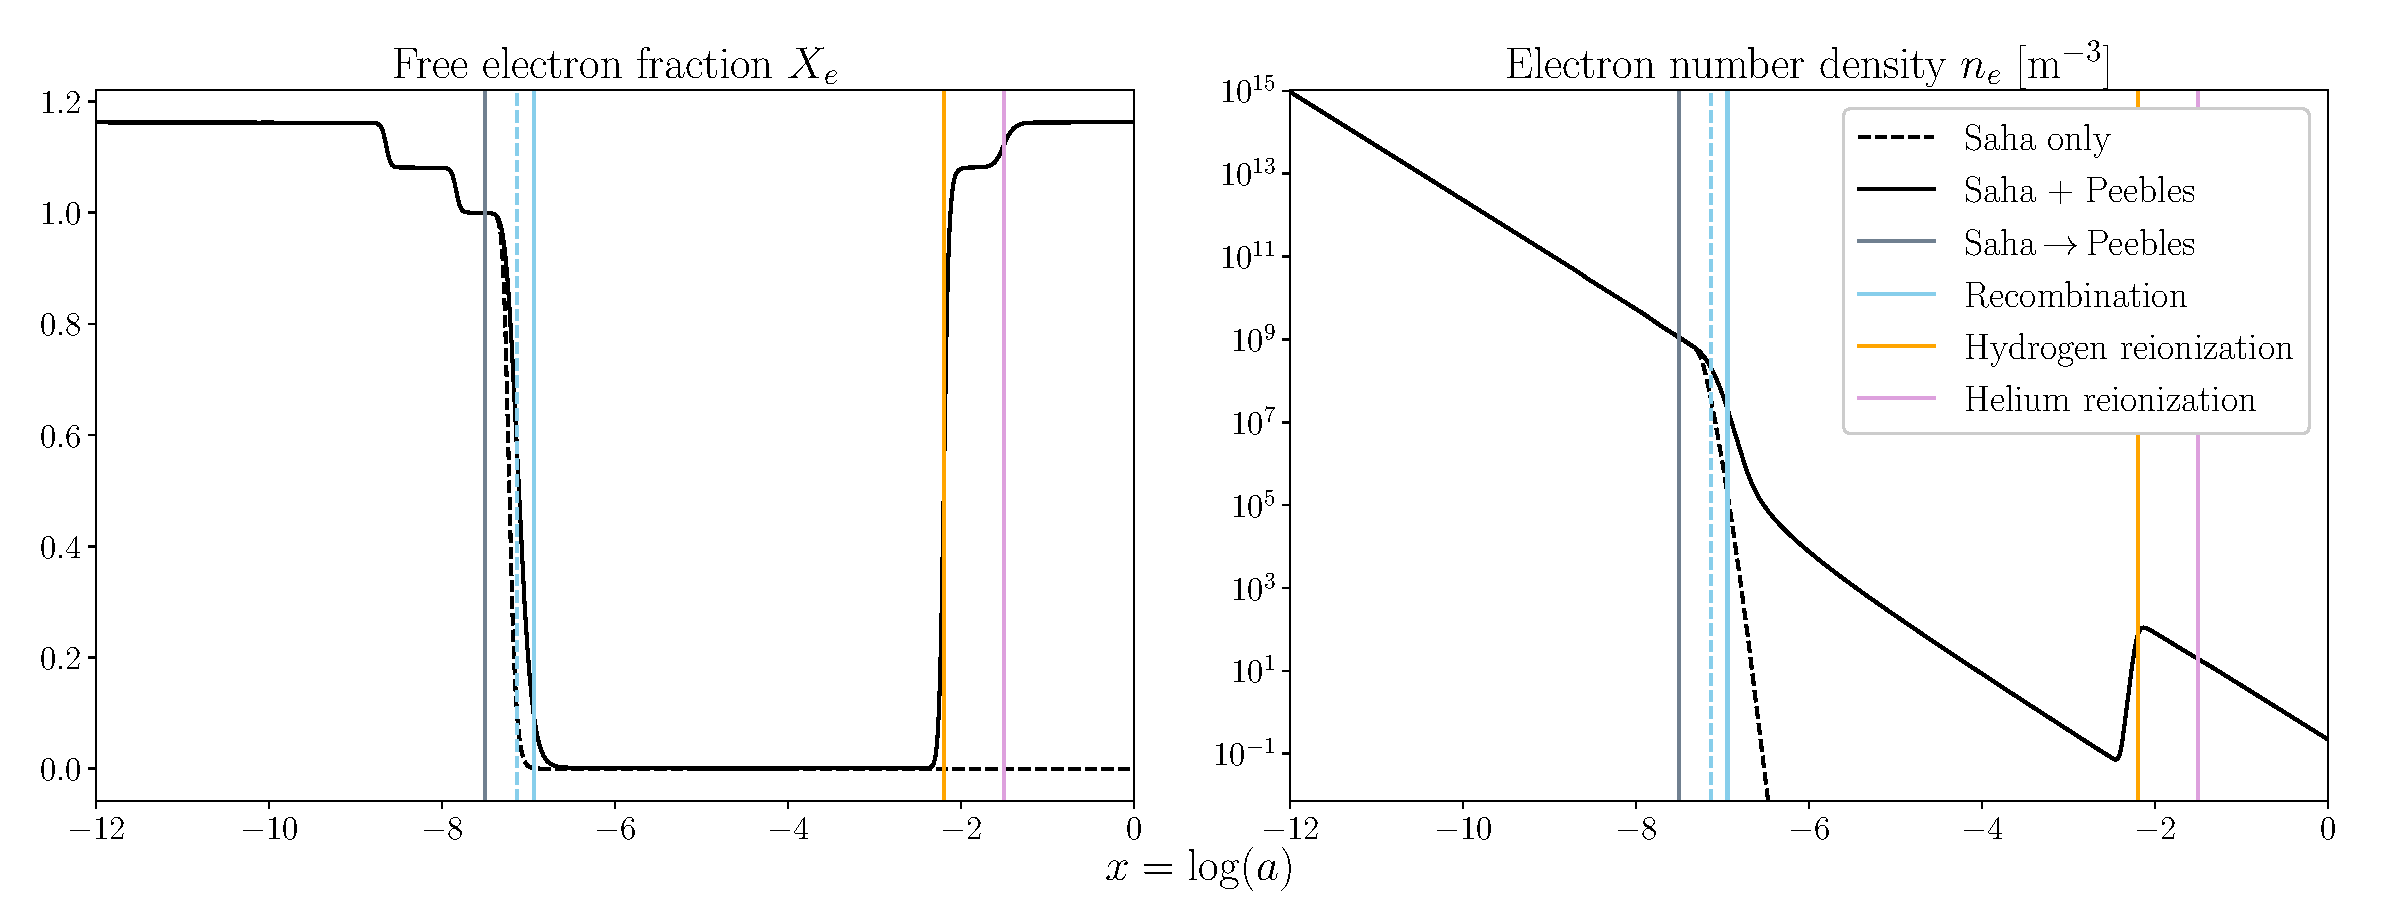
\includegraphics[width=\textwidth]{/Users/paljettrosa/Documents/GitHub/AST5220/figs/Xe_and_ne.pdf}
  \caption{The evolution of the free electron fraction $X_e$ (left) and the free electron number density $n_e$ (right) as functions of $x = \log(a)$. The dashed blue line indicates the time of recombination estimated using only the Saha approximation. The solid line show the result from solving the Peebles equation, and the significant difference illustrates the limitations of assuming equilibrium. The multiple orders of magnitude difference in $n_e$ and the sharp transitions highlight key epochs such as recombination, reionization, and helium reionization. \colorbox{Plum}{maybe remove last sentence}}\label{fig:X_e and n_e}
\end{figure*}

In figure \ref{fig:X_e and n_e} I have plotted the free electron fraction, $X_e$ (left subplot), and the electron number density, $n_e$ (right subplot), as a function of $x$. We see that $X_e \lesssim 1.2$ in the beginning when the Universe is fully ionized, slightly larger than 1 since we also have Helium. \colorbox{Plum}{maybe specify numbers} Furthermore, around 
$x \approx -9$, \colorbox{Plum}{correct?} doubly ionized Helium ($\text{He}^{++}$) recombines to singly ionized Helium ($\text{He}^+$), and shortly afterward, at $x \approx -8$, singly ionized Helium recombines to neutral Helium. At around $x\approx -7$ the free electron fraction rapidly drops as most electrons combine with protons to form neutral Hydrogen, proving Hydrogen recombination to be the dominant process. This is also very evident from the electron number density $n_e$, which decreases around four orders of magnitude during Hydrogen recombination, while no visible deviation from the usual volume dilution is visible during Helium recombination. colorbox{Plum}{word different?} Moreover, the dashed blue line indicates the expected recombination time based on the Saha approximation, which predicts recombination happening slightly earlier than in the full numerical solution, marked by the solid blue line. This discrepancy arises due to non-equilibrium effects included in the Peebles equation. \colorbox{Plum}{explain? maybe make own paragraph}

By turning off reionization I found that the freeze-out abundance of free electrons corresponds to
\begin{align*}
  X_e &\approx 2.7 \times10^{-4},
  \\
  n_e &\approx 5.2 \times10^{-5}\,\text{m}^{-3}.
\end{align*}
This is consistent with expectations from recombination theory, where only a small residual ionized fraction remains after Hydrogen recombination. \colorbox{Plum}{compare with common results?} However, it is clear from the figure that at later times ($x \lesssim -2$), the reionization of Hydrogen and neutral Helium occurs, driven by the formation of the first stars and quasars. This leads to the expected rise in $X_e$ back toward $\lesssim1.1$. Reionization of singly ionized Helium follows at even later times, completing around $x \approx -1.5$. This is associated with high-energy sources such as quasars, which provide sufficient ionizing photons to fully ionize Helium.\colorbox{Plum}{source} Although the free electron fraction does increase at this point, the overall change in the number density is negligible compared to the multiple orders of magnitude that it increases around the first reionization period, in agreement with the evolution around recombination. \colorbox{Plum}{word different/discuss implication}





\subsubsection{Optical depths}

\begin{figure*}
  \centering
  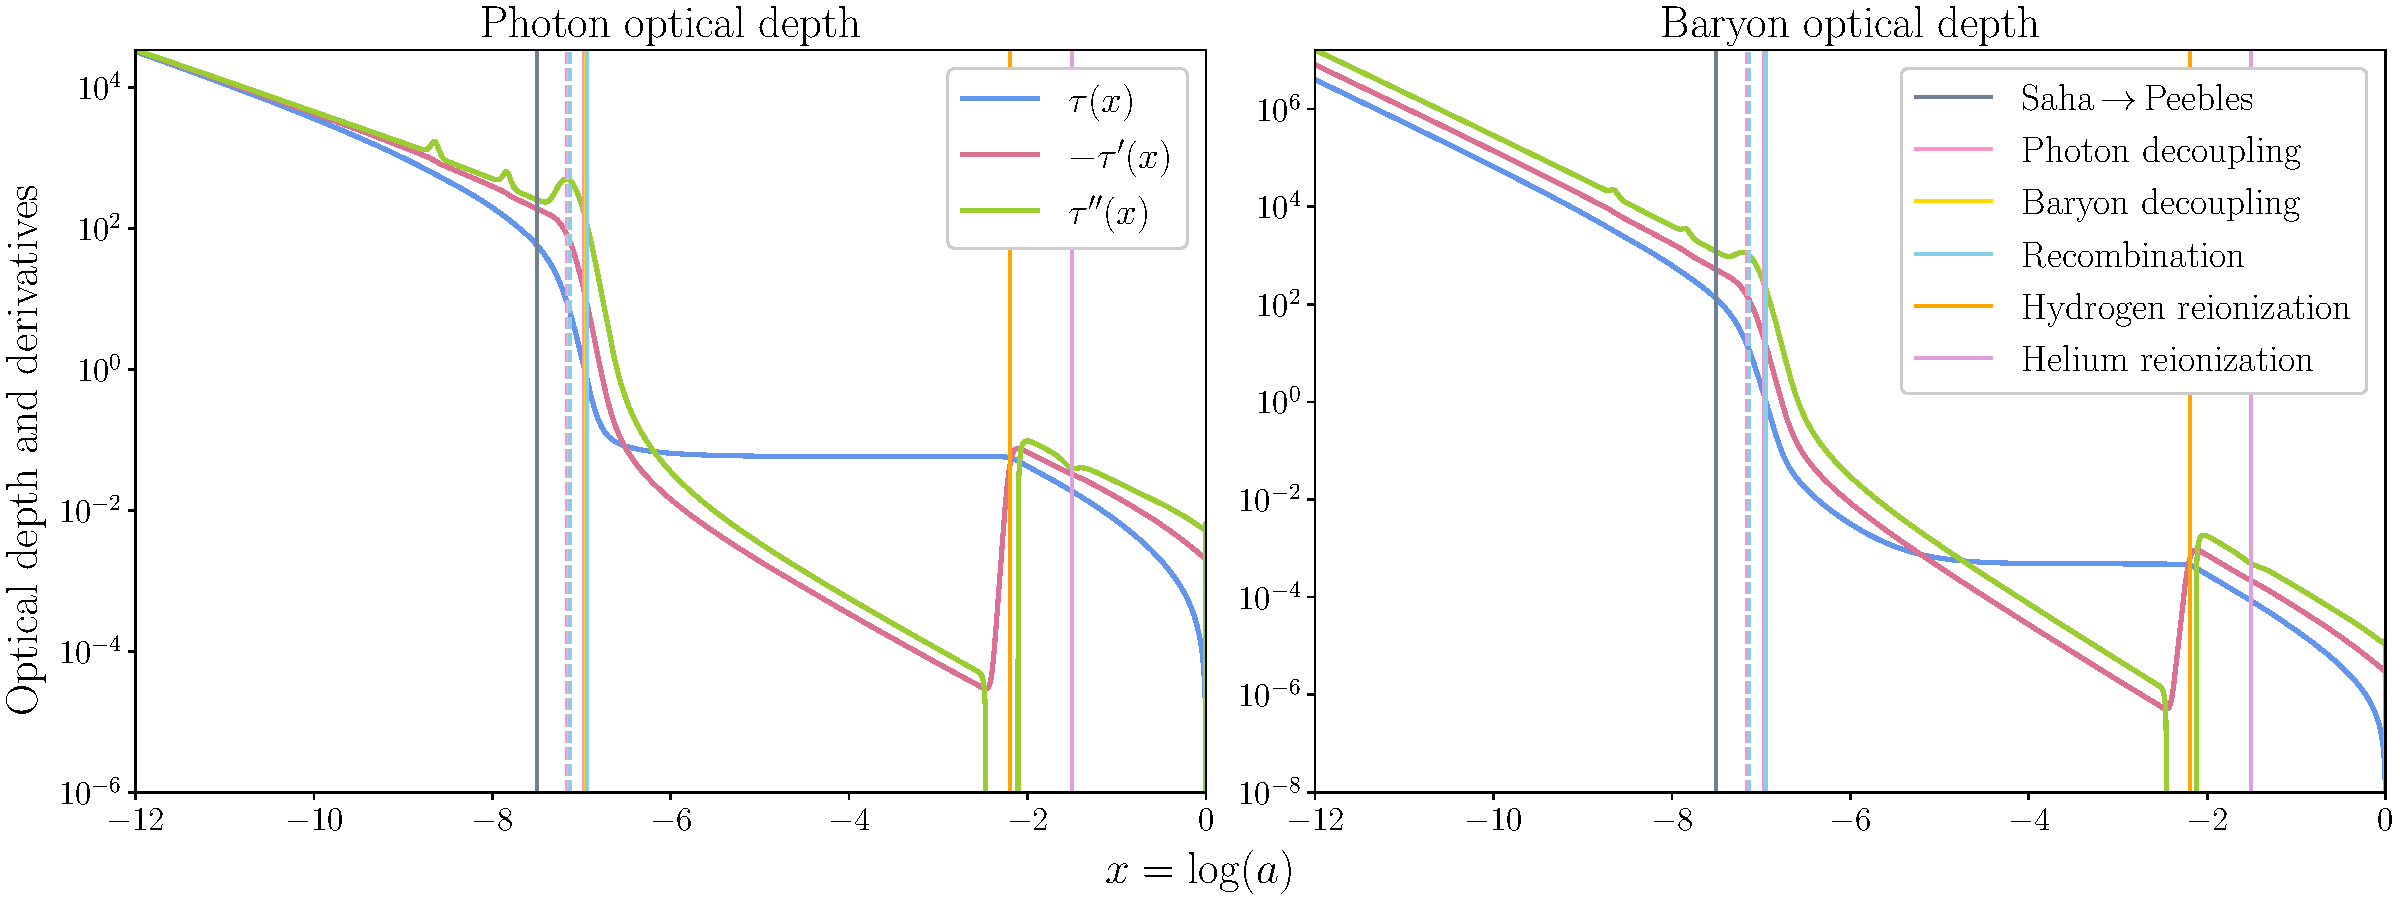
\includegraphics[width=\textwidth]{/Users/paljettrosa/Documents/GitHub/AST5220/figs/optical_depth.pdf}
  \caption{The evolution of the optical depth $\tau$ (blue), its first derivative $-\tau'$ (red), and its second derivative $\tau''$ (green) for both photons (darker lines) and baryons (lighter lines). The bottom left subplot shows the evolutions of these quantities around decoupling and recombination, while the bottom right subplot highlights their changes during the epoch of reionization. The drop in $\tau$ marks photon decoupling, while the gradual decline in $\tau_b$ reflects the extended drag epoch. Reionization leads to characteristic plateaus in the optical depths that extend towards late times.}\label{fig:optical depth}
\end{figure*}

Figure \ref{fig:optical depth} illustrates the evolution of the optical depth $\tau(x)$ (blue), its first derivative $-\tau'(x)$ (red), and its second derivative $\tau''(x)$ (green) as functions of $x$. These quantities are shown for both photons (darker colors) and baryons (lighter colors). We see that the photon optical depth $\tau$ is initially large, reflecting the fact that photons are tightly coupled to the baryon-electron plasma due to frequent Thomson scattering. Around decoupling we see a rapid drop in $\tau$, since the photons stop noticing the baryons. This is also visible from the steep negative peak in $-\tau'$, which marks the rapid decline in the scattering probability. Furthermore, the second derivative $\tau''$ has two smaller peaks before the large one right before recombination, highlighting the changes in the free electron fraction seen in figure \ref{fig:X_e and n_e}. Though subtle, the two smaller peaks indeed match sudden drops in $-\tau'$, which are directly linked to the abrupt changes in $n_e$ as electrons and $\text{He}^{++}$ form $\text{He}^{+}$ and later when neutral Helium is formed. \colorbox{Plum}{shorten/split into two?}

After recombination, $\tau$ levels off and remains roughly constant, meaning that photons are no longer frequently scattering. This corresponds to the transition to CMB free-streaming, where the photons released at decoupling can travel more or less uninterrupted throughout the Universe. We see a sudden increase in $-\tau'$ (and thus a sharp drop in $\tau''$) at $x \lesssim -2$ when ionizing radiation from early stars reionizes neutral Hydrogen, as this leads to a rapid increase in free electrons. This is reflected in the sharp increase in $n_e$ seen in figure \ref{fig:X_e and n_e}, and leads to the so-called reionization plateau \colorbox{Plum}{correct name?} we see in the graph for $\tau$. A second, smaller bump also occurs at $x \approx -1.5$ due to Helium reionization, where high-energy photons from quasars fully ionize Helium.

To understand the reionization plateau \colorbox{Plum}{correct name?}, we may imagine a photon released at some redshift $z<z_\text{reion}$. Since most electrons are free, the photon has a much larger probability of being scattered on its way towards us than if all the Hydrogen in the Universe was neutral. Thus, the longer ago that it was emitted, the larger this probability is, and thus the larger the optical depth. However, if it was emitted at some redshift $z_\text{rec}\gg z>z_\text{reion}$, where $z_\text{rec}$ is the redshift at recombination, this probability remains approximately constant up until reionization, hence why the optical depth does as well. \colorbox{Plum}{shorten/explain in theory?} The value of $\tau$ at reionization is often more interesting than the redshift at which it happened, and from my computed spline I found this to be  $\tau_\text{reion} = 0.0561$. This perfectly matches the Planck 2018 result: from $1\sigma$ limits on TT,TE,EE+lowE+lensing+BAO measurements, \cite{Planck} estimated the optical depth of this plateau as $\tau_\text{reion}=0.0561\pm0.0071$. \colorbox{Plum}{discuss, word differently?}. 

We see that the baryon optical depth $\tau_b$ behaves similarly to the photon optical depth but starts off having a much larger value, reflecting the fact that the photon-to-baryon ratio is very large, and the baryons thus have an even shorter mean free path than photons in the tightly coupled plasma. \colorbox{Plum}{word different?} It also has a longer tail due to the drag epoch, which is evident from the baryon decoupling occurring at a slightly later epoch than photon decoupling, as well as $-\tau_b$ falling off more gradually. The additional interactions between baryons and photons delay the time at which baryons move independently, which is important for setting the initial conditions for large-scale structure formation. While photons begin free-streaming immediately, baryons remain coupled to the residual ionized plasma for a longer time, affecting the formation of the first acoustic peaks in the CMB. \colorbox{Plum}{maybe shorten/move to theory} Furthermore, Hydrogen and Helium reionization cause a delayed but similar rise in the baryon optical depth derivative, just as in the photon case. The impact is, however, less pronounced because baryons are non-relativistic and are not as strongly affected by the free-electron fraction as photons.


\subsubsection{Visibility functions}

\begin{figure}
  \centering
  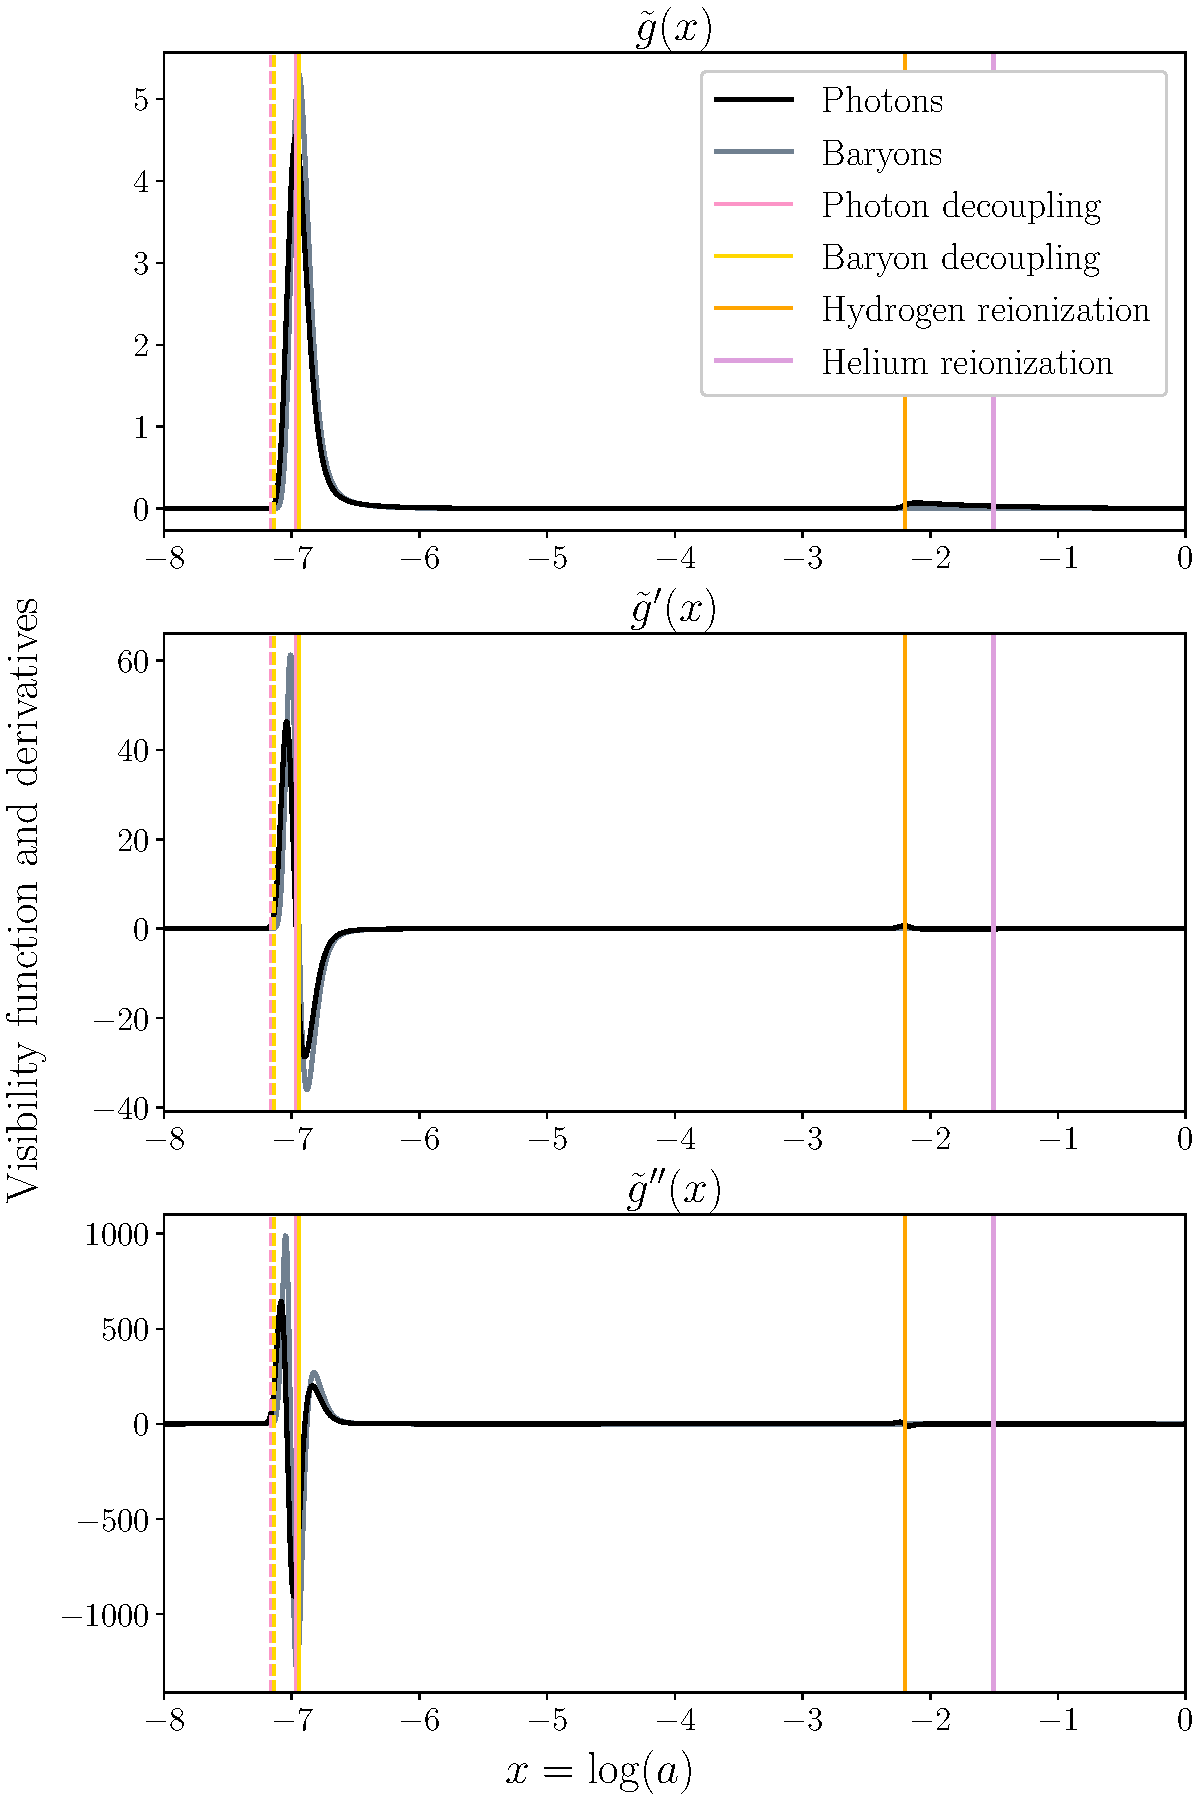
\includegraphics[width=\columnwidth]{/Users/paljettrosa/Documents/GitHub/AST5220/figs/visibility_function.pdf}
  \caption{The visibility function $\tilde{g}(x)$ (top), its first derivative $\tilde{g}'(x)$ (middle), and its second derivative $\tilde{g}''(x)$ (bottom), plotted for both photons (black) and baryons (grey). The sharp peak in $\tilde{g}$ defines the last scattering surface, while the first derivative's zero-crossing confirms the rapid transition. The second derivative provides insight into the smoothness of recombination, and secondary features at late times reflect reionization events. \colorbox{Plum}{maybe word differently}}\label{fig:visibility function}
\end{figure}

In figure \ref{fig:visibility function} I have plotted the photon (black) and baryon (grey) visibility functions $\tilde{g}(x)$ and $\tilde{g}_b(x)$ (top), their first derivatives $\tilde{g}'(x)$ and $\tilde{g}_b'(x)$ (middle), and their second derivatives $\tilde{g}''(x)$ and $\tilde{g}_b''(x)$ (bottom) as functions of $x$. I have cropped away the interval $x\in[-12,-8)$, since all the quantities stay constant at zero here. \colorbox{Plum}{okay to do this?} The large peaks of the visibility functions around $x \approx -7 $ agree with the estimated decoupling times, and we see that $\tilde{g}_b$ indeed peaks slightly later than $\tilde{g}$. Furthermore, this peak is significantly larger for $\tilde{g}_b$ than $\tilde{g}$, which reflects the fact that $\tau_b>\tau$ and $-\tau_b'>-\tau'$ around decoupling, as seen in figure \ref{fig:optical depth}. \colorbox{Plum}{word different} 

The width of the largest peak in the photon visibility function $\tilde{g}$ defines the thickness of the last scattering surface: a thinner peak would indicate an abrupt transition, while a broader peak suggests a more extended recombination \colorbox{Plum}{correct? move to theory?}. Furthermore, the peak of $\tilde{g}'$ corresponds to the moment of steepest decrease in the visibility function. Thus, the fact that the zero-crossing of $\tilde{g}'$ closely aligns with photon decoupling confirms that this was when the transition was most rapid. \colorbox{Plum}{maybe remove} The double derivative $\tilde{g}'' $ provides further insight into the smoothness of recombination, with a sharp peak indicating that recombination happened quickly, and a broader feature suggesting a more gradual transition. The strong negative dip around $ x \approx -7 $ thus reflects the sharpness of the last scattering surface, confirming that photon decoupling occurred in a well-defined window. \colorbox{Plum}{correct? move to theory?}


Around $x \lesssim -2$, Hydrogen reionization causes a secondary, broad increase in $ \tilde{g}(x)$, reflecting the renewed interaction between photons and free electrons. However, this increase is much smaller than at recombination, indicating that only a small fraction of the Universe's photons were re-scattered during this epoch. Even smaller is the change due to the reionization of $\text{He}^{+}$ to $\text{He}^{++}$, which matches the negligible effect on the optical depths and their first derivatives. Similar to why the changes in $\tilde{g}_b$ and its derivatives were larger than those of $\tilde{g}$ and its derivatives around decoupling, they are negligible in comparison at reionization. This reflects the significantly smaller magnitudes of $\tau_b$ and $\tau_b'$ in this region. \colorbox{Plum}{rewrite?}



\subsubsection{Important time stamps and horizons}

\begin{table*}
  \caption{Table of key cosmological time stamps, showing photon and baryon decoupling, the changes that occur inbetween (the drag epoch), and recombination, along with their corresponding redshifts, cosmic times, conformal times (particle horizons), and sound horizons. The Saha-only results differ significantly from the full solution, underestimating recombination time due to its equilibrium assumption.} 
  %The sound horizon at recombination sets the scale for acoustic peaks in the CMB and BAO in large-scale structure. \colorbox{Plum}{fact check} \colorbox{Plum}{add Planck values!}}             % title of Table
  \label{table:time stamps decoupling}    % is used to refer this table in the text
  \centering                          % used for centering table
  \begin{tabular}{| c || c || c | c | c | c |}        % centered columns (4 columns)
  \hline                % inserts double horizontal lines
  Quantity & Method & Photon decoupling & Baryon decoupling & Drag epoch & Recombination \\    % table heading 
  \hline\hline                        % inserts single horizontal line
  \multirow{2}{*}{$x$}       & Saha only       & \hspace{4.5pt}$-7.16$  & \hspace{4.5pt}$-7.14$     & \hspace{4.5pt}$0.02$        & \hspace{4.5pt}$-7.13$   \\      
  \cline{2-6}
                           & Saha + Peebles  & \hspace{4.5pt}$-6.97$  & \hspace{4.5pt}$-6.95$     & \hspace{4.5pt}$0.02$        & \hspace{4.5pt}$-6.94$   \\      
  \hline 
  \multirow{2}{*}{$z$}       & Saha only       & \hspace{-4pt}$1291.70$ & \hspace{-4pt}$1260.11$    & \hspace{-7pt}$-31.59$       & \hspace{-4pt}$1249.29$ \\
  \cline{2-6}
                           & Saha + Peebles  & \hspace{-4pt}$1064.44$ & \hspace{-4pt}$1037.76$    & \hspace{-7pt}$-26.68$       & \hspace{-4pt}$1033.21$ \\
  \hline 
  \multirow{2}{*}{$t$ [kyr]} & Saha only       & \hspace{1pt}$279.19$   & \hspace{1pt}$291.19$      & \hspace{-0.5pt}$11.99$        & \hspace{1pt}$295.48$    \\
  \cline{2-6}
                           & Saha + Peebles  & \hspace{1pt}$387.17$   & \hspace{1pt}$404.02$      & \hspace{-0.5pt}$16.85$      & \hspace{1pt}$407.01$    \\
  % \hline 
  % $\eta/c$ (Saha, TODO) & $934.94\,$Myr & \hspace{6pt}$949.53\,$Myr   & \hspace{0pt}$14.59\,$Myr  & \hspace{0pt}$14.59\,$Myr \\ 
  % \cline{2-6}
  % $\eta/c$ (numerical)  & $934.94\,$Myr & \hspace{6pt}$949.53\,$Myr   & \hspace{0pt}$14.59\,$Myr  & \hspace{0pt}$14.59\,$Myr TODO \\
  \hline 
  \multirow{2}{*}{$\eta$ [Mpc]} & Saha only       & \hspace{1pt}$246.80$   & \hspace{1pt}$251.49$      & \hspace{4.5pt}$4.69$        & \hspace{1pt}$253.14$    \\ 
  \cline{2-6}
                           & Saha + Peebles  & \hspace{1pt}$285.49$   & \hspace{1pt}$290.92$      & \hspace{4.5pt}$5.43$        & \hspace{1pt}$291.87$    \\ 
  \hline 
  \multirow{2}{*}{$s$ [Mpc]} & Saha only       & \hspace{1pt}$128.90$   & \hspace{1pt}$131.09$      & \hspace{4.5pt}$2.19$        & \hspace{1pt}$131.85$    \\ 
  \cline{2-6}
                           & Saha + Peebles  & \hspace{1pt}$146.66$   & \hspace{1pt}$149.10$      & \hspace{4.5pt}$2.44$        & \hspace{1pt}$149.53$    \\
  \hline                                   %inserts single line
  \end{tabular}
\end{table*}

Table \ref{table:time stamps decoupling} shows computed values of $x$, redshift $z$, cosmic time $t$, conformal time (particle horizon) $\eta$, and sound horizon $s$ corresponding to photon and baryon decoupling, the changes that occured between the two (drag epoch), and recombination. These have all been computed by using the Saha approximation only, and by using both Saha and the full Peebles equation. We see that photon decoupling (where the optical depth equals unity) and recombination (where the free electron fraction drops below 0.1) occur at nearly identical times. This is expected since photons cease scattering once hydrogen atoms form, meaning the two processes are closely linked. However, recombination occurs slightly earlier because a small number of free electrons remain after decoupling. \colorbox{Plum}{write different/remove?} 

Baryon decoupling happens at a slightly later time than photon decoupling, as evident from figures \ref{fig:optical depth} and \ref{fig:visibility function}. This is because, even after photons decouple, baryons still experience residual interactions due to photon pressure, preventing them from immediately falling into dark matter potential wells. The end of the drag epoch marks the transition from radiation-driven baryonic motion to gravitationally-driven structure formation. \colorbox{Plum}{remove?}

By using only the Saha approximation, both recombination and decoupling appear to happen much earlier, which agrees with the more sudden drop in the free electron fraction seen in figure \ref{fig:X_e and n_e}. This occurs because the Saha equation assumes instantaneous thermal equilibrium, meaning ionization and recombination happen instantly when crossing equilibrium thresholds. \colorbox{Plum}{correct?} In reality, the recombination process is non-instantaneous, as captured by the Peebles equation, which accounts for the slower capture of electrons by protons in an expanding universe.

The difference in sound horizons between the Saha-only approximation and the Saha + Peebles method shows that an earlier recombination leads to a slightly smaller horizon. This would have a direct impact on the CMB power spectrum, as the first acoustic peak corresponds to the largest mode that fits within the sound horizon at decoupling. Thus, a smaller sound horizon would shift the peak positions in the CMB anisotropy spectrum. It would also influence the baryon acoustic oscillations (BAO) in the matter power spectrum, which serves as a key probe of large-scale structure formation. This clearly shows the importance of using the Peebles equation to correctly model recombination, as the Saha approximation alone leads to artificially early decoupling. \colorbox{Plum}{word different?}

\colorbox{Plum}{rename section?}


\begin{figure}
  \centering
  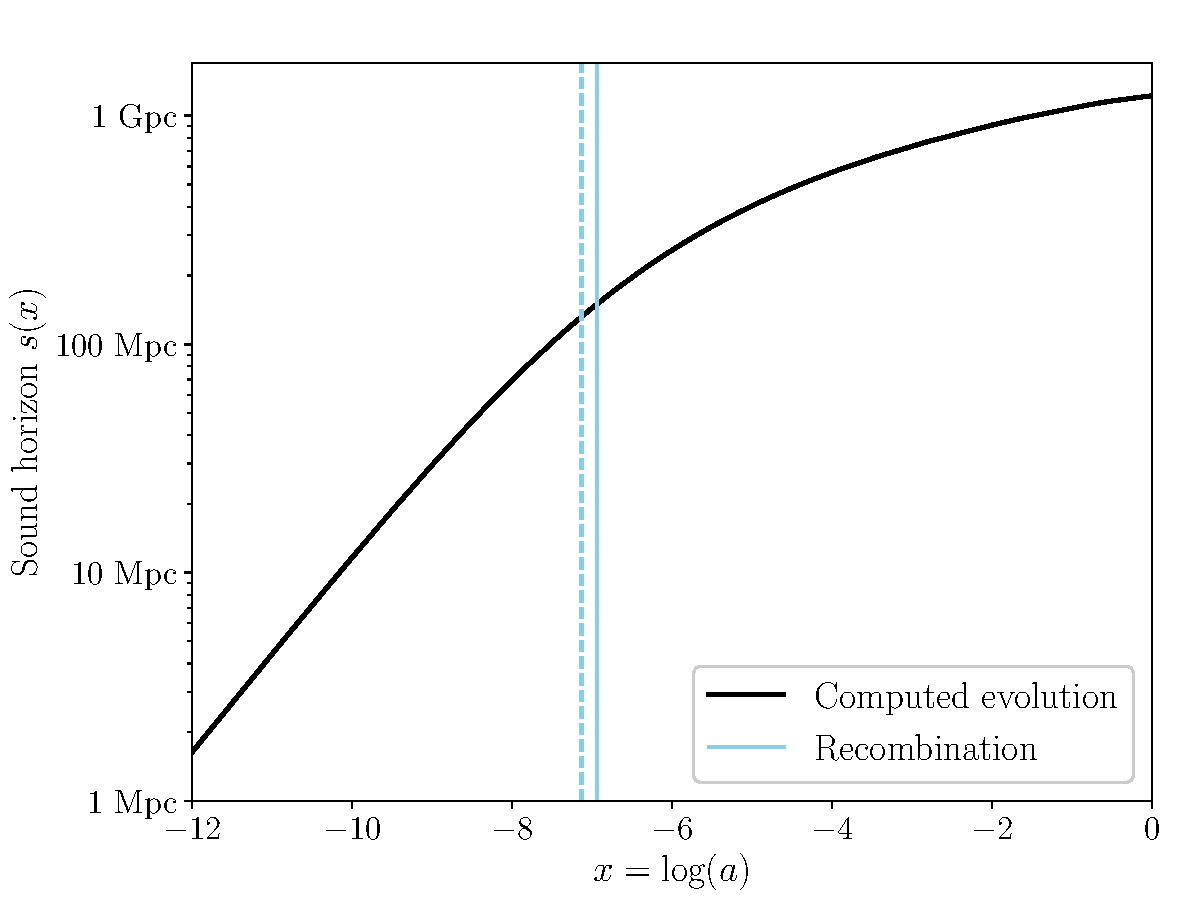
\includegraphics[width=\columnwidth]{/Users/paljettrosa/Documents/GitHub/AST5220/figs/sound_horizon.pdf}
  \caption{The evolution of the sound horizon $s(x)$ as a function of $x = \log(a)$. The rapid early growth reflects the high sound speed in the tightly coupled photon-baryon plasma, while the flattening at recombination marks the transition to the dark era. \colorbox{Plum}{correct?}}\label{fig:sound horizon}
\end{figure}

Figure \ref{fig:sound horizon} illustrates the evolution of the sound horizon $s(x)$, with the estimated time of recombination marked to highlight where the growth of the horizon gets stunted. \colorbox{Plum}{word different?} We see that $s$ grows rapidly at early times, which reflects the fact that sound waves in the tightly coupled photon-baryon fluid propagate at a relativistic speed. However, around recombination, the rate of photon-baryon interactions drops sharply. This weakens the pressure support from photons, allowing for clustering of matter and thus leading to a decline in the sound speed. \colorbox{Plum}{correct?} Consequently, the sound horizon's growth rate flattens out, as baryons start to decouple from photons and fall into dark matter potential wells. This is reflected in the less steep slope of $ s$ beyond recombination. \colorbox{Plum}{word differently}

In \cite{Planck}, the redshifts at photon and baryon decoupling are estimated to be $z_s=1089.92\pm0.25$ and $z_\text{drag} = 1059.94\pm0.30$, respectively, based on $1\sigma$ limits on TT,TE,EE+lowE+lensing measurements. The associated sound horizons were then $r_s=144.43\pm0.26$ and $r_\text{drag} = 149.09\pm0.26$. \colorbox{Plum}{discuss}

Using the value for the particle horizon at photon decoupling presented in table \ref{table:time stamps decoupling} (Saha + Peebles value), and the particle horizon today presented in table \ref{table:time stamps} (numerical value), we find that the comoving distance to the last scattering surface is
\begin{equation*}
  \chi_{s} = \eta_0-\eta_{s} \approx 13904.51\,\text{Mpc}.
\end{equation*}
Since I calculated the sound horizon at to be $r_s \approx 146.66\,\text{Mpc}$, the angular acoustic scale becomes
\begin{equation*}
  100\theta_{s} = 100\frac{r_s}{\chi_{s}} \approx 1.0548.
\end{equation*}
This is larger than the Planck result of $100\theta_{s}=1.0411\pm0.0003$, and not within their uncertainty. However, it should be noted that my inferred value really is not precise down to this number of decimals, because ... Nevertheless, this means that ...  \colorbox{Plum}{weave into rest of the text, discuss}

\colorbox{Plum}{maybe introduce expression in theory}

\colorbox{Plum}{mention that Planck has z-reion as 7.64?}




\subsubsection{Baryon temperature evolution}

\begin{figure}
  \centering
  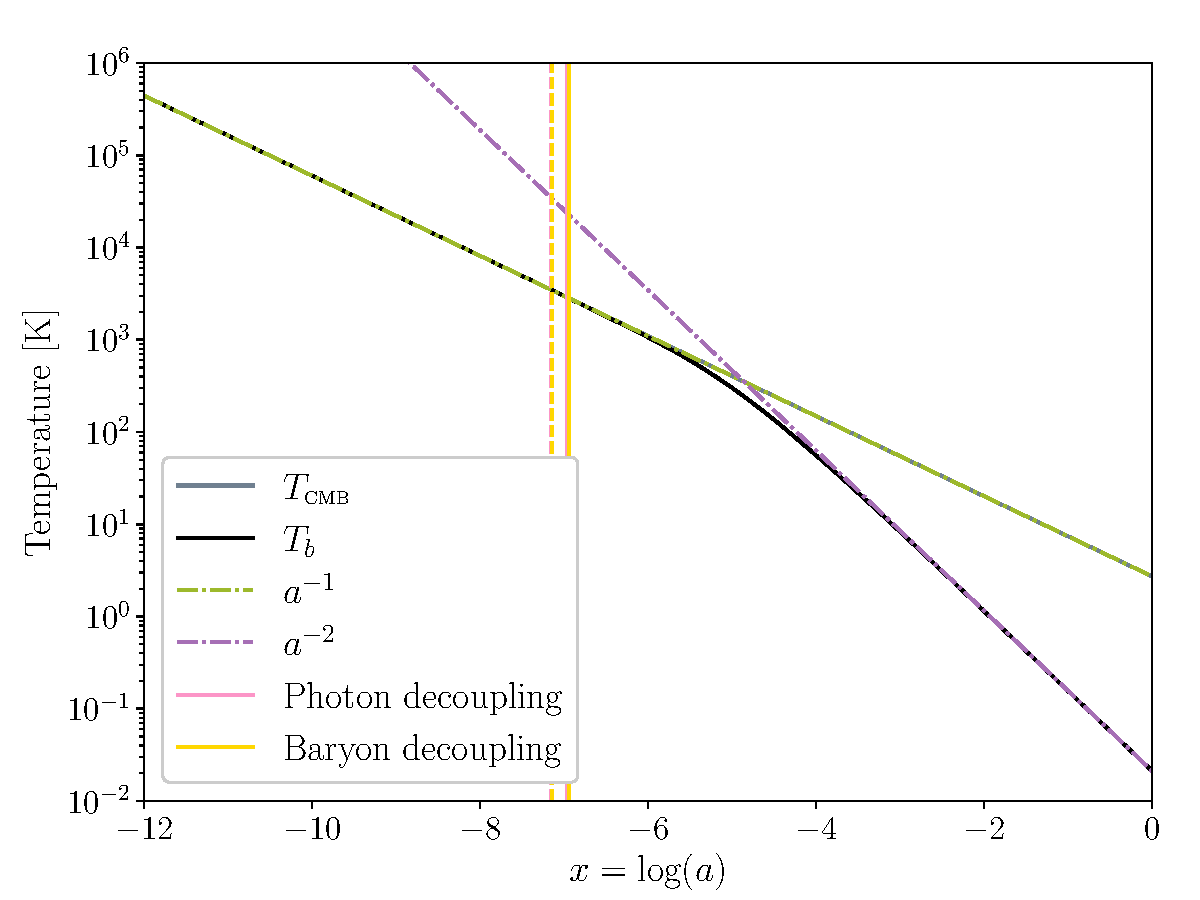
\includegraphics[width=\columnwidth]{/Users/paljettrosa/Documents/GitHub/AST5220/figs/photon_baryon_temp.pdf}
  \caption{The evolution of the baryon temperature $T_b(x)$ (black) compared to the photon temperature $T_\text{CMB}(x)$ (grey). The two temperatures track each other closely before recombination due to strong Thomson scattering. Some time after decoupling, baryons start to cool adiabatically as $T_b \propto a^{-2}$ \colorbox{Plum}{fact check}, while photons continue to cool as $T_\text{CMB} \propto a^{-1}$.}\label{fig:baryon temperature}
\end{figure}

In figure \ref{fig:baryon temperature} I have plotted the evolution of the baryon temperature $T_b$ (black line) and the photon (CMB) temperature $T_\text{CMB}$ (grey line) as functions of $x$. At early times ($x \lesssim -6$), the baryon temperature closely follows the photon temperature. This is expected since Thomson scattering between electrons and CMB photons efficiently transfers energy between the two components, maintaining thermal equilibrium. In this regime, both temperatures follow the expected radiation-like scaling, decreasing as $T\propto a^{-1}$ and thus following the green dashed line. 

% In figure \ref{fig:optical depth} we saw a sharp decrease in the optical depth around decoupling, due to Thomson scattering becoming inefficient after the free electron fraction drops. As a result, baryons are no longer in thermal equilibrium with photons, and the two temperatures begin to diverge. 
At around $x\approx-6$ the baryon temperature starts to evolve adiabatically, cooling faster than photons as $T_b\propto a^{-2}$, following the purple dashed line. This is directly linked to the drop in optical depth observed in the previous plots. As soon as photon interactions weaken, baryons begin cooling faster, confirming their thermal decoupling from the radiation field. The delay between decoupling and the point where the two diverge explains why $\tau_b$ declines more gradually than $\tau$ in figure \ref{fig:optical depth}, extending the impact of photon pressure beyond the formal decoupling time. \colorbox{Plum}{correct? word different?} 

At the present, I found the baryon temperature to be
\begin{equation*}
T_{b0} \approx 21.176\,\text{mK}.
\end{equation*}
This is significantly lower than the measured CMB temperature, which is $T_\text{CMB0} \approx 2.725 \,$K. The baryon temperature is therefore only $ \sim 7-8\% $ of the CMB temperature today, reflecting the expected $a^{-2}$ dependence during late times. \colorbox{Plum}{discuss more? find source of baryon temp?} This temperature deviation between photons and baryons introduces a slight correction to the photon-baryon sound speed, which could, in principle, affect acoustic oscillations in the CMB. However, this effect is likely quite small, as recombination is already more or less complete when $T_b$ begins deviating significantly from $T_\text{CMB}$. \colorbox{Plum}{move to theory?}








\section{Milestone III: Perturbations}\label{sec: milestone III}
Having established the background evolution of the universe and the recombination history in the previous milestones, I now turn to the evolution of cosmological perturbations, which describe how small fluctuations in density and temperature grew from the early universe into the large-scale structures we observe today. This step is essential for understanding the formation of the CMB anisotropies, as well as the distribution of galaxies and clusters in the late universe. \colorbox{Plum}{maybe remove}

In this milestone, I numerically solve the Einstein-Boltzmann equations to track the evolution of perturbations in different components of the Universe, including photons, neutrinos, baryons, and cold dark matter. By evolving these perturbations across different Fourier modes, I construct time-dependent solutions for key physical quantities such as density and velocity perturbations, temperature fluctuations, and gravitational potentials. Additionally, I account for the tight coupling approximation at early times to handle numerical instabilities and ensure accurate solutions. The results from this milestone provide the foundation for computing the CMB power spectrum in the next step, allowing us to directly compare theoretical predictions with observations.

\colorbox{Plum}{mention that we use linear perturbation theory}


\subsection{Theoretical framework}\label{subsec: III theory}

\begin{enumerate}
  \item [1.] Introduce the concept of metric perturbations by writing up the perturbed line element $ds^2$, and explain that the Einstein equations for scalars, vectors and tensors don't mix at linear order and can therefore be treated separately. I will mostly focus on scalar fluctuations and the associated density perturbations. Vector perturbations aren't produced by inflation and even if they were, they would decay quickly with the expansion of the Universe. Tensor perturbations (gravitational waves) are an important prediction of inflation and I will get back to them in the next milestone. 
  \item [2.] Explain that we use the Newtonian gauge because we then can apply some of our Newtonian intuition, and introduce the potentials $\Psi$ and $\Phi$. 
  \item [3.] Explain that the perturbation equations we end up with are going to be coupled linear partial differential equations, which are not trivial in real space, hence why we go to Fourier space. Explain that we go from spatial variables $v^i$ to wave vector components $k^i$, and that $\nabla u(x)\to i\vec{k}\tilde{u}(k)$ as we move to Fourier space.
  \item [4.] Introduce the perturbed Einstein-Boltzmann equation (the Boltzmann equation in general relativity that we introduced in the previous milestone) for photons, by stating the geodesic equation in a perturbed universe. Use this to show the momentum perturbations for photons today (subscript 0) as function of values at recombination (subscript rec): 
  \begin{equation}
    \left(\frac{\delta p}{p}\right)_0 = \left(\frac{\delta p}{p}\right)_\text{rec} + \left(\Psi_\text{rec} - \Psi_0\right) + \int_{t_\text{rec}}^{t_0}\left[\frac{\partial\Psi}{\partial t} - \frac{\partial \Phi}{\partial t} \right]\,dt,
  \end{equation}
  and identify and explain the Sachs-Wolfe and Integrated Sachs-Wolfe effects. Explain what these mean, and how important they are for understanding CMB anisotropies.
  \item [5.] Explain that by introducing perturbations in the temperature 
  \begin{equation}
    T=\overline{T}(1+\Theta(t,\vec{x},p,\hat{p})),
  \end{equation}
  and thus in the distribution function for photons (expand this in the $\Theta\ll1$ limit) we end with the Boltzmann equation with the background subtracted.
  \item [5.] Finally arrive at the explicit expressions for the photon temperature multipoles, using multipole expansions. Explain where these come from, and state the general expressions.
  \item [6.] Explain what the monopole, dipole and quadrupole represent.
  \item [7.] Explain how and why we truncate the Boltzmann hierarchies of infinite equations.
  \item [8.] Explain the concept of polarization of photons, and how the polarization spectra can be used to constrain parameters. 
  \item [9.] State the explicit polarization expressions in the problem description, and explain that we will further analyze the concept itself, the E-modes and B-modes (explain briefly what these are) and their spectra in the next milestone.
  \item [10.] Explain that this is very similar to the photon situation, but without polarization and a collision term. Explain also that neutrinos in reality have mass, and that it becomes significantly more complicated if we include this, hence why we ignore it.
  \item [11.] State the explicit expressions for the neutrino multipoles, and explain them.
  \item [12.] Derive the explicit expressions for cold dark matter density perturbations and velocity. See the lecture notes.
  \item [13.] Derive the explicit expressions for baryon density perturbations and velocity. See the lecture notes.
  \item [14.] Make sure to mention the interactions we can ignore/must include for baryons, hence why the collision term is not zero.
  \item [15.] Explain that the nonzero metric elements are
  \begin{align}
    g_{00} &= -\left(1+2\Psi \right),
    \\
    g_{ij} &= a^2\left(1+2\Phi \right)\delta_{ij},
  \end{align}
  and that, since the potentials $\Psi$ and $\Phi$ are small, the inverse metric components are
  \begin{align}
    g^{00} &= -\frac{1}{1+2\Psi} \simeq -1+2\Psi,
    \\
    g^{ij} &= \frac{1}{a^2\left(1+2\Phi \right)}\delta_{ij} \simeq a^{-2}\left(1-2\Phi\right)\delta_{ij}.
  \end{align}
  \item [16.] Move on to explain that after computing the Christoffel symbols, the Ricci tensor and scalar, and the Einstein tensor, we can move on to the general relativistic expression for the energy momentum tensor in the Boltzmann formalism:
  \begin{equation}
    T_\nu^\mu = \frac{g}{(2\pi)^3}\int\frac{dP_1dP_2dP_3}{\sqrt{-\text{det}\,g}}\frac{P^\mu P_\nu}{P^0}f,
  \end{equation}
  where $P^\mu=dx^\mu/d\lambda$ is the 4-momentum and $\text{det}\,g$ is the determinant of the metric $g_{\mu\nu}$. Show the approximate expression for this, using that it is diagonal, and explain that we can compute the $\mu=0$, $\nu=0$ component with $f=\overline{f}+\delta f$ to get
  \begin{align}
    \left(T_0^0\right)_\gamma &= -\overline{\rho}_\gamma\left(1+4\Theta_0\right),
    \\
    \left(T_0^0\right)_\nu &= -\overline{\rho}_\nu\left(1+4\mathcal{N}_0\right),
    \\
    \left(T_0^0\right)_\text{CDM} &= -\overline{\rho}_\text{CDM}\left(1+\delta_\text{CDM}\right),
    \\
    \left(T_0^0\right)_b &= -\overline{\rho}_b\left(1+\delta_b\right),
  \end{align}
  \item [17.] Explain then how this leads to the expressions for $\Phi'$ and $\Psi$ stated in the problem description. 
  \item [18.] Briefly explain what inflation is, why we need it (primarily horizon and flatness problem), and explain how this affects our initial conditions.
  \item [19.] State the initial conditions we will use, and explain where each of them come from.
  \item [20.] Explain what the tight-coupling regime is, why it introduces a problem for solving the full set of equations, and how we will combine the solution from this regime with the solution at later times to describe the entire process. 
  \item [21.] Derive the relevant expressions from the problem description, and explain where they come from and why they are more numerically stable.
  \item [22.] Tie the initial conditions together with the higher order $\ell\geq2$ multipole moments.
\end{enumerate}

% Points 1-3 are for subsection 1, points 4-9 for subsection 2, points 10 and 11 for subsection 3, 12 for subsection 4, 13 and 14 for subsection 5, 15-17 for subsection 6, 18 and 19 for subsection 7, and points 20-22 for subsection 8. 

% Can you write subsection 8 about the tight-coupling regime? Make sure to include points 20-22. Be concise and thorough, and match my writing style from the previous milestones.


\subsubsection{Metric perturbations}
\color{Plum}
In cosmology, we study the evolution of small fluctuations in the early universe to understand the formation of large-scale structure and CMB anisotropies. These fluctuations are described by perturbations to the metric, which we express as  
\begin{equation}
ds^2 = - (1 + 2\Psi) dt^2 + a^2 (1 + 2\Phi) \delta_{ij} dx^i dx^j.
\end{equation}
Here, $\Psi$ and $\Phi$ are the gravitational potentials, which describe scalar perturbations to the metric. The perturbed Einstein equations for scalars, vectors, and tensors decouple at linear order, allowing us to study them separately. In this work, we primarily focus on scalar perturbations, which correspond to density fluctuations and are responsible for structure formation.  

- Vector perturbations (vorticity) are not generated by inflation and decay rapidly due to cosmic expansion.  
- Tensor perturbations (gravitational waves) are a key prediction of inflation and will be studied in the next milestone.  

To simplify the perturbation equations, we work in the Newtonian gauge, where the metric is diagonal, and the gravitational potentials $\Psi$ and $\Phi$ play analogous roles to the Newtonian potential in classical gravity. The Newtonian gauge allows us to apply Newtonian intuition while keeping the full relativistic structure of general relativity. In this gauge:  

- $\Psi$ represents the perturbation to the time-time component of the metric and acts as the gravitational potential experienced by non-relativistic particles.  
- $\Phi$ appears in the spatial metric perturbations and affects the expansion of space.  

The Einstein equations relate these potentials to the density perturbations and the velocity divergence of different components in the universe. 

The perturbation equations take the form of coupled partial differential equations in real space, which are not trivial to solve. To simplify the problem, we transform them into Fourier space, where they become a system of ordinary differential equations (ODEs) for each wave mode. This is justified by the linearity of the system, allowing each mode to evolve independently.  

In Fourier space, spatial derivatives transform as:  
\begin{equation}
\nabla u(x) \rightarrow i \mathbf{k} \tilde{u}(k),
\end{equation}
where $\mathbf{k}$ is the comoving wave vector of the perturbation. This Fourier decomposition allows us to track the evolution of perturbations across different scales and study their behavior from superhorizon to subhorizon regimes.

Metric perturbations introduce small fluctuations to the FLRW metric, leading to the formation of structure in the universe. By adopting the Newtonian gauge, we simplify the system while retaining the key gravitational potentials, $\Psi$ and $\Phi$. Transforming to Fourier space further reduces the complexity, enabling efficient numerical evolution of perturbations. In the next section, we introduce the Boltzmann equation for photons and discuss how perturbations in the CMB temperature and momentum are generated, leading to the anisotropies we observe today.
\color{black}






\subsubsection{Photons}
\color{Plum}
The evolution of CMB anisotropies is governed by perturbations in the photon distribution function. Since photons are massless, they follow geodesics in a perturbed metric, meaning their evolution is described by the Einstein-Boltzmann equation. In this section, we derive the key equations governing photon perturbations, leading to the multipole expansion that describes temperature fluctuations observed in the CMB.  

The motion of photons in a perturbed universe is dictated by the geodesic equation, which describes how a photon's energy and momentum change due to metric perturbations. For a photon with four-momentum $P^\mu$, the geodesic equation in the perturbed Newtonian gauge metric takes the form:
\begin{equation}
\frac{dP^0}{d\lambda} + \Gamma^0_{\mu\nu} P^\mu P^\nu = 0.
\end{equation}
By expanding the Christoffel symbols and solving for small perturbations, we obtain the evolution of photon energy fluctuations. The perturbation to the photon momentum today (subscript 0) as a function of its value at recombination (subscript rec) is given by:
\begin{equation}
\left(\frac{\delta p}{p}\right)_0 = \left(\frac{\delta p}{p}\right)_{\text{rec}} + \left(\Psi_{\text{rec}} - \Psi_0\right) + \int_{t_{\text{rec}}}^{t_0} \left[\frac{\partial\Psi}{\partial t} - \frac{\partial \Phi}{\partial t} \right] dt.
\end{equation}
This equation encodes two key effects that shape CMB anisotropies:

1. The Sachs-Wolfe Effect: The gravitational redshift of photons due to metric perturbations at the last scattering surface. The term $(\Psi_{\text{rec}} - \Psi_0)$ represents the change in the gravitational potential from recombination to today.
2. The Integrated Sachs-Wolfe (ISW) Effect: The time variation of the metric perturbations $(\partial_t \Psi - \partial_t \Phi)$, which affects photon energy as they travel through evolving potential wells. This effect is most important in the late universe when dark energy becomes significant.

These effects contribute to large-scale temperature fluctuations in the CMB, directly imprinting information about early-universe physics and cosmic structure formation.

To systematically describe perturbations in the CMB, we introduce the photon temperature perturbation $\Theta$, defined as:
\begin{equation}
T = \overline{T} (1 + \Theta),
\end{equation}
where $\Theta(x, t, p, \hat{p})$ represents small deviations from the background photon temperature $\overline{T}$. Expanding the distribution function for photons in the limit $\Theta \ll 1$ gives:
\begin{equation}
f = f_0 + \frac{df_0}{dT} \Theta.
\end{equation}
Subtracting the background evolution, we obtain the Boltzmann equation for photons in perturbation form:
\begin{equation}
\frac{d\Theta}{dt} + \hat{p}^i \nabla_i \Theta + \frac{d\Phi}{dt} = C[f],
\end{equation}
where $C[f]$ is the collision term, which accounts for interactions between photons and electrons.

Since photons scatter with electrons before recombination, their perturbations must be expanded in multipole moments to track their angular dependence. Expanding the temperature perturbation in Legendre polynomials,
\begin{equation}
\Theta(\mathbf{k}, \hat{p}, t) = \sum_{\ell} (-i)^\ell (2\ell + 1) \Theta_\ell (k, t) P_\ell(\mu),
\end{equation}
we obtain the hierarchy of equations describing the evolution of photon perturbations. The first three moments correspond to:

- Monopole ($\ell = 0$): The mean temperature perturbation of the CMB, related to density fluctuations.
- Dipole ($\ell = 1$): Related to the bulk velocity of photons, which sources the Doppler effect.
- Quadrupole ($\ell = 2$): Represents anisotropic scattering and is crucial for generating CMB polarization.

Higher-order moments describe finer angular features of the CMB but decrease in importance due to Silk damping (photon diffusion).

The Boltzmann hierarchy consists of an infinite set of coupled equations, making numerical integration impractical. To solve the system efficiently, we truncate the hierarchy at some finite $\ell$, typically using a closure approximation:
\begin{equation}
\Theta_{\ell_{\max}} = \frac{2\ell_{\max} + 1}{k \eta} \Theta_{\ell_{\max} - 1}.
\end{equation}
This ensures that the higher-order multipoles decay smoothly, allowing for accurate numerical solutions while maintaining computational efficiency.

CMB photons are partially polarized due to Thomson scattering before recombination. Polarization is described by a Stokes parameter decomposition, where we define E-mode and B-mode polarization:

- E-modes: Even-parity polarization patterns sourced by scalar perturbations.
- B-modes: Odd-parity modes, generated primarily by gravitational waves (tensor perturbations).

Polarization spectra provide additional constraints on cosmological parameters, particularly on reionization history and primordial gravitational waves. In this milestone, we compute the linearized polarization evolution, leaving a more detailed discussion of B-modes for the next milestone.

In this section, we derived the Boltzmann equation for photons, showing how metric perturbations influence CMB anisotropies through the Sachs-Wolfe effect and ISW effect. We introduced the Legendre multipole expansion, leading to the Boltzmann hierarchy for temperature fluctuations. To close the system, we apply a truncation scheme that ensures numerical stability. Finally, we introduced the concept of photon polarization, which provides additional constraints on early-universe physics. In the next section, we extend this framework to include neutrino perturbations, which evolve similarly to photons but lack a collision term.
\color{black}







\subsubsection{Neutrinos}
\color{Plum}
Neutrinos play a crucial role in the evolution of cosmological perturbations due to their relativistic nature in the early universe and their free-streaming behavior after decoupling. Their evolution follows a similar structure to photon perturbations but differs in key aspects, particularly the absence of a collision term in the Boltzmann equation. In this section, we derive the perturbation equations for neutrinos and discuss their impact on the formation of large-scale structure and the CMB. 

Like photons, neutrinos follow the Einstein-Boltzmann equation, which describes the evolution of their phase-space distribution function $f_\nu$. In the absence of interactions, the Boltzmann equation for neutrinos simplifies to the collisionless form:
\begin{equation}
\frac{df_\nu}{dt} + \hat{p}^i \nabla_i f_\nu + \frac{d\Phi}{dt} \frac{\partial f_\nu}{\partial p} = 0.
\end{equation}
This equation shows that neutrino perturbations are affected by the gravitational potential $\Phi$ but evolve independently after decoupling. Unlike photons, which experience Thomson scattering with electrons, neutrinos interact only through the weak force and decouple much earlier, when the universe was around 1 second old.

Since neutrinos are relativistic in the early universe, their perturbations are best described using a Legendre multipole expansion, analogous to photons:
\begin{equation}
\mathcal{N}(\mathbf{k}, \hat{p}, t) = \sum_{\ell} (-i)^\ell (2\ell + 1) \mathcal{N}_\ell (k, t) P_\ell(\mu),
\end{equation}
where $\mathcal{N}_\ell$ are the multipole moments of the neutrino temperature perturbation. The hierarchy of equations governing these moments is given by:
\begin{equation}
\dot{\mathcal{N}}_0 = -k \mathcal{N}_1 - \dot{\Phi},
\end{equation}\begin{equation}
\dot{\mathcal{N}}_1 = \frac{k}{3} \left(\mathcal{N}_0 - 2 \mathcal{N}_2 \right) + k \Psi,
\end{equation}\begin{equation}
\dot{\mathcal{N}}_2 = \frac{k}{5} \left(2 \mathcal{N}_1 - 3 \mathcal{N}_3 \right).
\end{equation}
Higher-order moments follow the same recursion structure, similar to photons. However, due to the lack of a collision term, the neutrino quadrupole $\mathcal{N}_2$ is not suppressed like in the photon case, leading to enhanced free-streaming effects that impact structure formation. 

Since neutrinos do not interact with the photon-baryon plasma after decoupling, they free-stream out of overdensities, damping small-scale fluctuations. This has two key effects on cosmological evolution:

1. Damping of Small-Scale Perturbations:  
   Neutrino free-streaming prevents the formation of structure on scales smaller than the free-streaming length, suppressing power in the matter power spectrum at small scales.

2. Contribution to the Gravitational Potential:  
   Relativistic neutrinos contribute to the total energy density, affecting the growth rate of perturbations and shifting the phasing of acoustic oscillations in the CMB power spectrum.

In this analysis, we assume massless neutrinos, which simplifies their evolution. However, in reality, neutrinos have a small but finite mass, which introduces additional complexity:

- Massive neutrinos transition to a non-relativistic regime, altering their free-streaming behavior.
- Neutrinos with mass affect structure formation, contributing to the total matter density and modifying the growth of cosmic structures.

Since incorporating massive neutrinos requires solving the full phase-space evolution with a time-dependent equation of state, we neglect neutrino mass in this milestone for simplicity. 

Neutrino perturbations evolve similarly to photon perturbations but differ in key ways due to their collisionless nature. Their free-streaming behavior suppresses small-scale fluctuations and influences the gravitational potential, leaving an imprint on both CMB anisotropies and large-scale structure formation. In the next section, we derive the perturbation equations for cold dark matter, which forms the gravitational backbone of cosmic structure and evolves differently from relativistic species.
\color{black}







\subsubsection{Cold dark matter}
\color{Plum}
Cold dark matter (CDM) plays a crucial role in the formation of cosmic structure. Unlike photons and neutrinos, CDM particles are non-relativistic and interact only through gravity, meaning they do not experience pressure support or free-streaming effects. This leads to a different evolution for CDM perturbations, which gravitationally attract baryons and seed the formation of galaxies and large-scale structure.

Since CDM particles are massive and move non-relativistically, their phase-space distribution function is well approximated by the collisionless Boltzmann equation:
\begin{equation}
\frac{df_{\text{CDM}}}{dt} + \frac{dx^i}{dt} \frac{\partial f_{\text{CDM}}}{\partial x^i} + \frac{d p^i}{dt} \frac{\partial f_{\text{CDM}}}{\partial p^i} = 0.
\end{equation}
Because CDM particles interact only gravitationally, their velocity is governed by the geodesic equation in a perturbed metric:
\begin{equation}
\frac{d v^i}{dt} = -\nabla^i \Psi.
\end{equation}
Transforming to Fourier space and taking the first moments of the Boltzmann equation, we obtain the evolution equations for the CDM density contrast $\delta_{\text{CDM}}$ and velocity divergence $\theta_{\text{CDM}}$:
\begin{equation}
\dot{\delta}_{\text{CDM}} + \theta_{\text{CDM}} = 3 \dot{\Phi},
\end{equation}\begin{equation}
\dot{\theta}_{\text{CDM}} + H \theta_{\text{CDM}} = k^2 \Psi.
\end{equation}
Here:
- $\delta_{\text{CDM}} = \frac{\delta\rho_{\text{CDM}}}{\bar{\rho}_{\text{CDM}}}$ is the fractional overdensity of CDM,
- $\theta_{\text{CDM}}$ is the velocity divergence,
- $\Psi$ is the gravitational potential sourced by matter perturbations.

Unlike photons and neutrinos, which experience pressure or free-streaming effects, CDM perturbations grow unimpeded once they enter the horizon. This allows dark matter overdensities to deepen gravitational wells, which later pull in baryons and form galaxies and cosmic structure.

In the radiation-dominated era, perturbation growth is suppressed because radiation dominates the gravitational potential. However, once the universe becomes matter-dominated, CDM perturbations grow linearly with the scale factor:
\begin{equation}
\delta_{\text{CDM}} \propto a.
\end{equation}
This growth is crucial for explaining the observed cosmic web of galaxies and clusters in the late universe.

Cold dark matter provides the gravitational backbone for cosmic structure formation. Its perturbations evolve differently from those of photons and neutrinos, growing continuously without pressure support or free-streaming effects. The next section introduces the evolution of baryon perturbations, which experience additional interactions with photons and play a direct role in shaping the observable structure of the universe.
\color{black}






\subsubsection{Baryons}
\color{Plum}
Baryons, unlike cold dark matter (CDM), experience interactions with photons through Thomson scattering, making their evolution more complex. Before recombination, baryons are tightly coupled to photons, behaving as part of a single fluid with radiation. However, after recombination, baryons decouple and begin to fall into the gravitational potentials seeded by dark matter, leading to the formation of galaxies and large-scale structure.

The perturbations in the baryon density $\delta_b$ and velocity divergence $\theta_b$ evolve according to the Boltzmann equation, modified by interactions with photons. In Fourier space, the evolution equations are:
\begin{equation}
\dot{\delta}_b + \theta_b = 3\dot{\Phi},
\end{equation}
\begin{equation}
\dot{\theta}_b + H \theta_b = k^2 \Psi + R \left( \frac{4}{3} \theta_\gamma - \theta_b \right).
\end{equation}

Here:
- $\delta_b = \frac{\delta\rho_b}{\bar{\rho}_b}$ is the baryon density contrast,
- $\theta_b$ is the baryon velocity divergence,
- $\theta_\gamma$ is the photon velocity divergence,
- $R = \frac{3\rho_b}{4\rho_\gamma}$ quantifies the relative importance of baryons compared to radiation.

The key difference between baryons and CDM is the presence of the photon drag term proportional to $R$, which accounts for the transfer of momentum between photons and baryons. Before recombination, this term dominates, forcing baryons to move with photons in acoustic oscillations. After recombination, photons free-stream away, and the baryon velocity decouples, allowing baryons to fall into CDM potential wells.

Unlike CDM, which is collisionless, baryons experience Thomson scattering with photons until recombination. This means the collision term in the Boltzmann equation is nonzero and must be included. However, after recombination, the photon mean free path becomes large, making Thomson scattering negligible, and the baryons transition to behaving like a pressureless fluid.

Baryon perturbations are initially dominated by interactions with photons, leading to acoustic oscillations in the photon-baryon plasma. After recombination, baryons decouple and begin to collapse into dark matter potential wells, eventually forming galaxies and cosmic structures. The next section focuses on metric perturbations and their role in linking matter fluctuations to the gravitational potential.
\color{black}





\subsubsection{Metric potentials}
\color{Plum}
The evolution of density perturbations in the universe is directly linked to metric perturbations, which describe how spacetime responds to fluctuations in matter and radiation. In the Newtonian gauge, these perturbations are encoded in the gravitational potentials $\Psi$ and $\Phi$, which appear in the perturbed metric:
\begin{equation}
g_{00} = -\left(1 + 2\Psi \right), \quad g_{ij} = a^2\left(1 + 2\Phi \right)\delta_{ij}.
\end{equation}
Since the perturbations are small, the inverse metric components are approximated as:
\begin{equation}
g^{00} \simeq -1 + 2\Psi, \quad g^{ij} \simeq a^{-2} \left(1 - 2\Phi\right) \delta_{ij}.
\end{equation}
These potentials are sourced by the energy-momentum tensor of the universe's components, which can be derived using the Boltzmann formalism.

The perturbed energy-momentum tensor for a species with phase-space distribution function $f$ is given by:
\begin{equation}
T^\mu_\nu = \frac{g}{(2\pi)^3} \int \frac{d^3P}{\sqrt{-\det g}} \frac{P^\mu P_\nu}{P^0} f.
\end{equation}
Here, $P^\mu$ is the four-momentum, and $\det g$ is the determinant of the metric. Expanding this expression for different components, we obtain the $(0,0)$ component (energy density perturbations):
\begin{align}
  \left(T_0^0\right)_\gamma &= -\overline{\rho}_\gamma\left(1+4\Theta_0\right),
  \\
  \left(T_0^0\right)_\nu &= -\overline{\rho}_\nu\left(1+4\mathcal{N}_0\right),
  \\
  \left(T_0^0\right)_\text{CDM} &= -\overline{\rho}_\text{CDM}\left(1+\delta_\text{CDM}\right),
  \\
  \left(T_0^0\right)_b &= -\overline{\rho}_b\left(1+\delta_b\right),
\end{align}
These expressions show how different species contribute to the total energy density perturbation, which in turn determines the evolution of the metric potentials.

Using the perturbed Einstein equations, we obtain the key relations governing the evolution of $\Phi$ and $\Psi$. The Poisson equation relates the metric potential $\Psi$ to the total density perturbation:
\begin{equation}
k^2 \Phi = 4\pi G a^2 \sum_i \bar{\rho}_i \delta_i.
\end{equation}
Additionally, the evolution of the metric potentials is influenced by anisotropic stress. In the absence of significant stress (which is true for non-relativistic species), we have $\Psi = \Phi$, simplifying the system.

Metric perturbations encode the gravitational response to density fluctuations and play a crucial role in structure formation and cosmic microwave background (CMB) anisotropies. By linking the gravitational potentials $\Psi$ and $\Phi$ to the energy-momentum tensor, we establish a self-consistent system governing the evolution of matter, radiation, and geometry. In the next section, we introduce inflationary initial conditions, which set the stage for the growth of these perturbations.
\color{black}






\subsubsection{Inflation and initial conditions}
\color{Plum}
The initial conditions for cosmological perturbations are set during the inflationary era, a period of rapid exponential expansion in the early universe. Inflation provides a mechanism for generating the nearly scale-invariant density fluctuations observed in the CMB and large-scale structure. These fluctuations originate from quantum fluctuations in the inflaton field, which were stretched to macroscopic scales by inflation and later evolved into the perturbations we observe today.

Inflation solves several fundamental problems of the standard Big Bang model:

- Horizon problem: The CMB is observed to be nearly uniform across the sky, despite regions being causally disconnected in a non-inflationary scenario. Inflation ensures that all observable regions were once in causal contact.
- Flatness problem: The observed spatial curvature of the universe is extremely close to zero ($\Omega_k \approx 0$), which inflation naturally explains by driving the universe toward spatial flatness.
- Exotic relics problem: The rapid expansion dilutes unwanted relics, such as magnetic monopoles, that would otherwise dominate the energy density.

These features make inflation the leading paradigm for setting up the initial conditions of structure formation.

The key prediction of inflation is the generation of an almost scale-invariant power spectrum for the curvature perturbation $ \mathcal{R} $, given by:
\begin{equation}
P_\mathcal{R}(k) = A_s k^{n_s - 1},
\end{equation}
where $ A_s $ is the amplitude of scalar fluctuations, and $ n_s \approx 0.96 $ is the spectral index. These fluctuations set the initial conditions for all cosmological perturbations.

For adiabatic initial conditions, all species share the same density fluctuations:
\begin{equation}
\frac{\delta\rho_i}{\rho_i} = \frac{\delta\rho_j}{\rho_j} \quad \forall i, j.
\end{equation}
This means that initial perturbations affect all components (photons, baryons, dark matter, neutrinos) in a correlated way, ensuring a consistent evolution.

At early times, when perturbations are on superhorizon scales ($ k \ll aH $), their evolution is well-approximated by a set of simple relations derived from the Einstein equations:
\begin{equation}
\Phi = \Psi = \text{constant},
\end{equation}\begin{equation}
\delta_{\text{CDM}} = \delta_b = -2\Phi,
\end{equation}\begin{equation}
\delta_\gamma = \delta_\nu = -2\Phi, \quad \theta_\gamma = \theta_\nu = -\frac{k^2 \eta}{2} \Phi.
\end{equation}
These conditions ensure that all components evolve consistently at early times. For the photon-baryon fluid, additional considerations related to tight coupling must be included, as discussed in the next section.

Inflation provides the primordial seeds for structure formation, generating nearly scale-invariant fluctuations that evolve into the observed cosmic web. The initial conditions for cosmological perturbations are derived from inflationary predictions and are imposed at early times when perturbations are on superhorizon scales. In the next section, we discuss the tight-coupling approximation, which allows us to handle the evolution of the tightly coupled photon-baryon plasma before recombination.
\color{black}






\subsubsection{The tight-coupling regime}
\color{Plum}
Before recombination, photons and baryons are strongly coupled through Thomson scattering, meaning that the mean free path of photons is extremely short compared to the horizon size. This tight coupling prevents photons from free-streaming and causes the photon-baryon fluid to behave as a single tightly coupled system. However, this strong interaction introduces a numerical challenge when solving the Boltzmann hierarchy, requiring a specialized approximation to maintain numerical stability.

In the tight-coupling regime, the photon-baryon system can be treated as a single fluid with a sound speed given by:
\begin{equation}
c_s^2 = \frac{1}{3(1 + R)},
\end{equation}
where $R = \frac{3\rho_b}{4\rho_\gamma}$ quantifies the relative importance of baryons compared to photons. Since the photons dominate the energy density, the sound speed is initially close to $1/\sqrt{3}$ but decreases as baryons become more significant.

To solve the Boltzmann hierarchy efficiently, we expand the equations in powers of the scattering rate $\dot{\kappa}$, where:
\begin{equation}
\dot{\kappa} = n_e \sigma_T a
\end{equation}
is the differential optical depth, controlling the rate of interactions between photons and electrons. In the tight-coupling limit, $\dot{\kappa} \gg H$, meaning that photons scatter rapidly and the system maintains a near-equilibrium configuration.

By expanding the photon dipole moment $\Theta_1$ in orders of $1/\dot{\kappa}$, we obtain an approximate solution for its evolution:
\begin{equation}
\Theta_1 = \frac{\theta_b}{3} + \mathcal{O}\left(\frac{1}{\dot{\kappa}}\right).
\end{equation}
This approximation allows us to bypass numerical stiffness in the early universe while retaining the essential physics of acoustic oscillations in the photon-baryon fluid.

As recombination progresses, the photon mean free path increases, and tight coupling becomes less valid. The transition is characterized by a breakdown of the approximation when $\dot{\kappa}$ becomes comparable to the expansion rate $H$. At this point, photons begin to free-stream, leading to:

- Silk damping, where small-scale fluctuations are erased due to photon diffusion.
- The emergence of CMB anisotropies, as photons decouple from baryons and travel freely.

To ensure a smooth numerical transition from tight coupling to free streaming, we match the approximate solution in the tight-coupling regime with the full Boltzmann hierarchy at later times.

The tight-coupling approximation allows us to handle the early evolution of the photon-baryon plasma efficiently, ensuring numerical stability when solving the Boltzmann equations. This approximation is valid until the onset of recombination, when photons begin to free-stream, forming the temperature anisotropies observed in the cosmic microwave background (CMB). By correctly implementing this transition, we ensure that our model accurately captures the evolution of perturbations across all relevant epochs.
\color{black}

Can you rewrite this so that all subsections go well together? I still want them divided the way they are now, but I want them to flow better into each other. Avoid repeating too much between each subsection. For example, when you introduce an equation where some variable appears, you do not have to explain what it is unless it has not yet been introduced in the text. Also, it is very important that you use exactly the same notation as in the lecture notes and problem description I uploaded. Lastly, every single one of the expressions in the boxes have to be included! For example, in the photon section, all expressions regarding the photon temperature and photon polarization have to written out explicitly (except for the initial conditions, which of course should be stated in the section about inflation and initial conditions).





\subsection{Implementation details}\label{subsec: III methods}

\subsection{Results and discussions}\label{subsec: III results}







\section{Milestone IV: Power Spectra}\label{sec: milestone IV}
Having explored the background evolution of the universe, its ionization history, and the growth of perturbations, we now reach the final step: computing the primary statistical observables in cosmology—the CMB power spectrum and the matter power spectrum. These spectra encode the evolution of perturbations from their initial conditions to their imprint on the cosmic microwave background and the large-scale distribution of matter. Their precise computation allows us to compare theoretical predictions with observations from missions such as Planck, placing stringent constraints on cosmological parameters.  

The CMB power spectrum quantifies temperature and polarization anisotropies in the CMB sky, which arise from acoustic oscillations in the early universe, gravitational redshifting, and scattering effects. To compute this spectrum, we must perform line-of-sight integration, tracing how photons have propagated from recombination to today, incorporating contributions from Sachs-Wolfe effects, Doppler shifts, and polarization terms. The matter power spectrum, on the other hand, describes how density fluctuations in the universe are distributed across different scales today. It is derived from the total matter perturbations, including contributions from dark matter and baryons, and plays a crucial role in understanding the formation of large-scale structure.  

By synthesizing the physics from all previous milestones, this milestone brings us to the final stage of our Einstein-Boltzmann solver. The results will allow direct comparison with observational data, testing the validity of our theoretical model and its numerical implementation.

\colorbox{Plum}{shorten}




\subsection{Theoretical framework}\label{subsec: IV theory}
\begin{enumerate}
  \item [1.] Explain how we can write the photon temperature field in terms of spherical harmonics, and define what these are.
  \item [2.] Explain why the CMB power spectrum is the square of the coefficients in the spherical harmonics expansion, and explain what the $\ell$'s and $m$'s mean. Explain also explicitly why there is no $m$-dependence, and we therefore write $C_\ell$.
  \item [3.] Explain thoroughly what the line-of-sight integration method is, who developed it, how it works and why it works.
  \item [4.] Explain and derive explicitly what the source function is, and explain that this comes from the milestone III result. Explain what each term means, where they come from and how they affect the power spectrum.
  \item [5.] Explain what the spherical bessel functions are, and why we use these when we perform line-of-sight integration (take into account the projection of the 3D characterized by $k$ onto a 2D sphere characterized by $\ell$).
  \item [6.] Explain how we can use the spline of the photon temperature and polarization multipoles to obtain the CMB power spectra for temperature and polarization, repsectively. Explain also the differences between the TT, TE and EE maps.
  \item [7.] Write explicitly the general expression for the primordial power spectrum, and explain where it comes from.
  \item [8.] Explain that most inflation models predict a so-called Harrison-Zel'dovich primordial spectrum, and explicitly write out the form of this. 
  \item [9.] Explain what cosmic variance is, state the expression for it and explain how it will inevitably affect the results.
  \item [10.] Explain how we can generate a CMB map with the help of the theoretical $C_\ell$ spectrum.
  \item [11.] Explain how we compute the neutrino power spectrum, and why it is similar to the CMB spectrm. Write explicitly out the source function.
  \item [12.] Explain what the matter power spectrum represents, and state the general expression for it. 
  \item [13.] Explain what the gauge invariant matter density field is, and why we need it.
  \item [14.] Explain how we can look at the matter power spectrum for individual components and state the general expression for $\Delta_i(k,x)$. Explain the terms.
  \item [15.] Explain what the correlation function is (Fourier transform of the matter power-spectrum), and what it represents. Explain how we easily can compute it. Motivate that it is interesting to study because of baryon acoustic oscillations?
  \item [16.] Explain what the angular correlation function is, and state the expression from the problem description appendix.
  \item [17.] Explain how we can compute the effects of gravitational lensing on the CMB temperature power spectrum, and write explicitly the expression for the lensed correlation function. Also write explicitly what $\sigma^2(\theta)$, $C_\text{gl}(\theta)$ and $C_\text{gl,2}(\theta)$ are, and what they physically represent. Also write out the expression for the reduced Wigner functions $d_{mn}^\ell(\theta)$. 
  \item [18.] Explain why the effects of gravitational lensing are interesting, and how we expect it to affect the power spectrum.
\end{enumerate}
% Points 1 and 2 are for subsection 1 (temperature fluctuations as spherical harmonics), points 3-5 for subsection 2 (line-of-sight integration), points 6-10 for subsection 3 (the CMB power spectra), point 11 for subsection 4 (the neutrino power spectrum), points 12-14 for subsection 5 (the matter power spectrum), point 15 for subsection 6 (the correlation function), and points 16-18 for subsection 7 (effects of gravitational lensing).

% Can you write subsection 7 about the effects of gravitational lensing? Make sure to include points 16-18: 
% \item [16.] Explain what the angular correlation function is, and state the expression from the problem description appendix.
% \item [17.] Explain how we can compute the effects of gravitational lensing on the CMB temperature power spectrum, and write explicitly the expression for the lensed correlation function. Also write explicitly what $\sigma^2(\theta)$, $C_\text{gl}(\theta)$ and $C_\text{gl,2}(\theta)$ are, and what they physically represent. Also write out the expression for the reduced Wigner functions $d_{mn}^\ell(\theta)$. 
% \item [18.] Explain why the effects of gravitational lensing are interesting, and how we expect it to affect the power spectrum.



\subsubsection{Temperature fluctuations as spherical harmonics}
\color{Plum}
The CMB temperature field is a function of direction on the sky, denoted by $\hat{n}$. This function, $\Theta(\hat{n})$, represents the temperature fluctuations in different directions and is defined as:  
\begin{equation}
T(\hat{n}) = \bar{T} (1 + \Theta(\hat{n})),
\end{equation}
where $\bar{T} \approx 2.725$ K is the mean CMB temperature, and $\Theta(\hat{n})$ describes small deviations from this mean due to primordial fluctuations.  

Since the observed CMB sky is a sphere, the most natural way to express these fluctuations is through an expansion in spherical harmonics $Y_{\ell m}(\hat{n})$, which form a complete set of orthonormal basis functions on the sphere:
\begin{equation}
\Theta(\hat{n}) = \sum_{\ell=0}^{\infty} \sum_{m=-\ell}^{\ell} a_{\ell m} Y_{\ell m} (\hat{n}).
\end{equation}
Here:  
- $\ell$ represents the multipole moment, corresponding to an angular scale $\theta \sim 180^\circ / \ell$.  
- $m$ determines the modes within a given multipole moment.  
- $Y_{\ell m}(\hat{n})$ are spherical harmonics, which form an orthonormal basis on the sphere:  
  \begin{equation}
  \int d\Omega Y_{\ell m}^*(\hat{n}) Y_{\ell' m'} (\hat{n}) = \delta_{\ell \ell'} \delta_{m m'}.
  \end{equation}
The coefficients $a_{\ell m}$ describe the contribution of each mode to the temperature fluctuations and are given by:
\begin{equation}
a_{\ell m} = \int d\Omega \Theta(\hat{n}) Y_{\ell m}^*(\hat{n}).
\end{equation}
Since the early-universe fluctuations are Gaussian random fields, the power spectrum fully characterizes their statistical properties. 

To quantify the strength of temperature fluctuations at each angular scale, we define the CMB power spectrum as:
\begin{equation}
C_\ell = \langle |a_{\ell m}|^2 \rangle.
\end{equation}
This measures the variance of the spherical harmonic coefficients over different realizations of the universe. In an isotropic universe, there is no preferred direction, so the expectation value is independent of $m$, leading to:
\begin{equation}
C_\ell = \frac{1}{2\ell+1} \sum_{m=-\ell}^{\ell} |a_{\ell m}|^2.
\end{equation}
This result follows from the statistical isotropy of the CMB, which ensures that all $m$-modes for a given $\ell$ contain equal power on average.  

The multipole moment $\ell$ determines the angular scale of fluctuations:
- Large scales (low $\ell$) correspond to super-horizon perturbations at recombination.
- Small scales (high $\ell$) probe sub-horizon physics, such as acoustic oscillations and Silk damping.

The power spectrum $C_\ell$ is the primary observable in CMB experiments, providing direct constraints on cosmological parameters such as the Hubble constant, dark matter density, baryon content, and primordial perturbations.

In the next section, we will discuss the line-of-sight integration method, which provides an efficient way to compute the CMB power spectrum from the underlying perturbation evolution.
\color{black}





\subsubsection{Line-of-sight integration}
\color{Plum}
The line-of-sight integration method is a computationally efficient approach to solving the Boltzmann hierarchy for the evolution of CMB anisotropies. Rather than solving an infinite set of coupled differential equations for multipole moments $\Theta_\ell$, this method directly computes the temperature and polarization power spectra by integrating along the photon trajectory from last scattering to today.  

This method was developed by Seljak and Zaldarriaga (1996) and is implemented in the widely used Boltzmann solvers such as CMBFAST, CAMB, and CLASS. It significantly reduces the numerical complexity of computing the CMB power spectrum by focusing on the key physical contributions to observed anisotropies.

The temperature perturbation in Fourier space can be written as an integral over conformal time $\eta$:
\begin{equation}
\Theta_{\ell}(k) = \int d\eta S_T(k, \eta) j_\ell(k (\eta_0 - \eta)).
\end{equation}
Here:
- $S_T(k, \eta)$ is the source function, which contains all physical effects contributing to temperature anisotropies.  
- $j_\ell(x)$ are spherical Bessel functions, describing how 3D perturbations in $k$-space project onto the 2D CMB sky.  

The power spectrum is then obtained from:
\begin{equation}
C_\ell^{TT} = \int dk \frac{k^2}{2\pi^2} P_{\mathcal{R}}(k) \Theta_{\ell}^2(k).
\end{equation}
This approach effectively compresses the evolution of perturbations into a single integral, avoiding the need to track each individual multipole separately.

The source function $S_T(k, \eta)$ determines the temperature anisotropies and is derived from the Boltzmann equation for photons. It is given by:
\begin{equation}
S_T(k, \eta) = e^{-\tau} \left[ \dot{\tau} \left( \Theta_0 + \Psi + \frac{1}{4} \Pi \right) + \dot{\Psi} - \dot{\Phi} \right].
\end{equation}
Each term represents a different physical contribution:

- Primary anisotropies:  
  - $\Theta_0$ is the monopole temperature fluctuation (density perturbations).  
  - $\Psi$ is the gravitational potential, contributing via the Sachs-Wolfe effect.  
  - $\frac{1}{4} \Pi$ is the quadrupole moment, which sources polarization.  

- Dynamical effects:  
  - $\dot{\Psi} - \dot{\Phi}$ encodes the Integrated Sachs-Wolfe (ISW) effect, which arises from the evolution of metric perturbations.  

- Visibility function:  
  - $\dot{\tau} e^{-\tau}$ is the visibility function, determining when photons last scatter. It peaks at recombination, meaning the largest contribution comes from this epoch.

The presence of $e^{-\tau}$ ensures that perturbations after recombination are exponentially suppressed due to photon free-streaming.

The transition from 3D perturbations in $k$-space to 2D temperature fluctuations on the sky is governed by spherical Bessel functions $j_\ell(x)$. These functions arise naturally when solving the Helmholtz equation in spherical coordinates and describe how plane waves project onto a spherical surface.  

The argument of the Bessel function,
\begin{equation}
x = k (\eta_0 - \eta),
\end{equation}
represents the comoving distance traveled by a photon since a given time $\eta$.  

- Large scales (small $k$):  
  - $j_\ell(x)$ peaks at small $x$, meaning large-scale perturbations contribute mostly to low $\ell$.  
- Small scales (large $k$):  
  - Higher $k$-modes lead to oscillations in $j_\ell(x)$, corresponding to the acoustic peaks in the CMB power spectrum.  

Since the line-of-sight integral involves a sum over many oscillatory contributions, features in the power spectrum (such as acoustic peaks) emerge from constructive and destructive interference of these modes.

The line-of-sight integration method transforms the Boltzmann hierarchy into a single integral, significantly improving computational efficiency. The source function encapsulates the key physical effects driving CMB anisotropies, while the spherical Bessel functions handle the projection from 3D perturbations to 2D anisotropies. This formalism enables accurate and efficient computation of the CMB temperature and polarization power spectra, which we explore in the next section.
\color{black}





\subsubsection{The CMB power spectra}
\color{Plum}
The CMB power spectra provide the primary statistical observables for studying the early universe, capturing information about the temperature and polarization anisotropies imprinted on the cosmic microwave background (CMB). These spectra encode the physics of the primordial perturbations, the evolution of the photon-baryon plasma, and the effects of recombination and reionization.  

From the line-of-sight integral solution discussed in the previous section, the temperature and polarization multipoles $\Theta_\ell(k)$ and $E_\ell(k)$ are computed as functions of wavenumber $k$ and conformal time $\eta$. Since these multipoles oscillate due to acoustic physics in the early universe, we interpolate their evolution using cubic splines to achieve a smooth and accurate representation of their values at different times.  

Once the multipoles are known, the temperature (TT), polarization (EE), and cross-correlation (TE) power spectra are computed as:
\begin{equation}
C_\ell^{XY} = \int dk \frac{k^2}{2\pi^2} P_{\mathcal{R}}(k) X_\ell(k) Y_\ell(k),
\end{equation}
where $X, Y$ can be either $\Theta_\ell$ (temperature) or $E_\ell$ (polarization), and $P_{\mathcal{R}}(k)$ is the primordial power spectrum.  

The three main CMB power spectra are:  
- TT spectrum $C_\ell^{TT}$: Measures the temperature fluctuations of the CMB.  
- EE spectrum $C_\ell^{EE}$: Quantifies the E-mode polarization generated by Thomson scattering before recombination.  
- TE spectrum $C_\ell^{TE}$: Represents the correlation between temperature and E-mode polarization.  

Since polarization is generated only in scattering events, the TE correlation provides valuable information about reionization and the last scattering epoch.  

The power spectrum of perturbations today depends on the initial conditions set by inflation. The primordial curvature power spectrum, denoted by $P_{\mathcal{R}}(k)$, describes the initial amplitude of perturbations as a function of wavenumber $k$:
\begin{equation}
P_{\mathcal{R}}(k) = A_s \left(\frac{k}{k_*}\right)^{n_s - 1}.
\end{equation}
Here:
- $A_s$ is the scalar amplitude, setting the overall normalization.  
- $n_s$ is the spectral index, determining the tilt of the spectrum.  
- $k_*$ is a pivot scale, typically chosen at $k_* = 0.05 \, \text{Mpc}^{-1}$ for CMB experiments.  

The primordial power spectrum provides the input for all structure formation models, influencing both CMB anisotropies and large-scale structure.

Most inflationary models predict an approximately scale-invariant spectrum, known as the Harrison-Zel'dovich spectrum. This corresponds to a spectral index of:
\begin{equation}
n_s = 1.
\end{equation}
In this case, the primordial power spectrum simplifies to:
\begin{equation}
P_{\mathcal{R}}(k) = A_s.
\end{equation}
This means that perturbations are seeded equally at all scales, leading to a nearly scale-invariant distribution of density fluctuations. However, Planck observations indicate that $n_s \approx 0.96$, meaning that small-scale perturbations are slightly suppressed compared to large scales, favoring slightly red-tilted spectra.

Since we only observe one realization of the CMB sky, our measurement of $C_\ell$ is subject to cosmic variance. This statistical uncertainty arises because we have access to a finite number of modes at each multipole $\ell$. The standard deviation in $C_\ell$ due to cosmic variance is given by:
\begin{equation}
\frac{\Delta C_\ell}{C_\ell} = \sqrt{\frac{2}{2\ell+1}}.
\end{equation}
This effect is most pronounced at low multipoles ($\ell < 30$), where there are fewer independent modes available. As a result, large-scale features in the CMB (such as the Sachs-Wolfe plateau) are inherently noisier compared to smaller-scale acoustic peaks.

Given the theoretical prediction for the CMB power spectrum $C_\ell$, we can generate simulated CMB maps by drawing random realizations from a Gaussian distribution:
\begin{equation}
a_{\ell m} \sim \mathcal{N}(0, C_\ell).
\end{equation}
By expanding these random coefficients in spherical harmonics:
\begin{equation}
\Theta(\hat{n}) = \sum_{\ell m} a_{\ell m} Y_{\ell m} (\hat{n}),
\end{equation}
we obtain synthetic CMB maps that statistically resemble the observed sky. These maps are crucial for testing theoretical models, estimating errors, and designing observational strategies. 

The CMB power spectra encapsulate the physics of the early universe, encoding information about primordial fluctuations, acoustic oscillations, reionization, and large-scale structure formation. The TT, TE, and EE spectra are computed using the spline-interpolated multipoles from the Boltzmann solver. The primordial power spectrum serves as the initial condition for perturbation growth, and cosmic variance limits our precision at large scales. Finally, simulated CMB maps provide an essential tool for understanding and interpreting observational data.  

In the next section, we extend this formalism to compute the neutrino power spectrum, which follows a similar structure but incorporates unique free-streaming effects.
\color{black}






\subsubsection{The neutrino power spectrum}
\color{Plum}
Neutrinos play a crucial role in shaping the evolution of cosmological perturbations. Since they decouple from the primordial plasma while still relativistic, they free-stream across cosmic distances, influencing the growth of large-scale structure and leaving a distinct imprint on the matter and CMB power spectra. The neutrino power spectrum quantifies the statistical distribution of neutrino perturbations, analogous to the CMB power spectrum for photons.

The neutrino power spectrum is computed using the same line-of-sight formalism as the CMB, but with key differences due to the absence of a collision term in the Boltzmann equation. The temperature fluctuations for neutrinos are expanded in spherical harmonics, just as for photons:
\begin{equation}
\mathcal{N}(\hat{n}) = \sum_{\ell m} \mathcal{N}_{\ell m} Y_{\ell m} (\hat{n}).
\end{equation}
The neutrino multipoles $\mathcal{N}_\ell(k)$ evolve according to the same line-of-sight integral method:
\begin{equation}
\mathcal{N}_\ell(k) = \int d\eta \, S_{\nu}(k, \eta) j_\ell(k (\eta_0 - \eta)).
\end{equation}
Here:
- $S_{\nu}(k, \eta)$ is the neutrino source function, encoding the physics of neutrino anisotropies.  
- $j_\ell(x)$ are spherical Bessel functions, handling the projection from 3D $k$-space to 2D angular fluctuations.  

The neutrino power spectrum is then given by:
\begin{equation}
C_\ell^{\nu\nu} = \int dk \frac{k^2}{2\pi^2} P_{\mathcal{R}}(k) \mathcal{N}_\ell^2(k).
\end{equation}
This formulation is nearly identical to the CMB power spectrum computation, but the source function differs due to the collisionless evolution of neutrinos.

The source function for neutrino perturbations follows from the Boltzmann equation for collisionless, relativistic species:
\begin{equation}
S_{\nu}(k, \eta) = e^{-\tau_\nu} \left[ \dot{\Psi} - \dot{\Phi} \right].
\end{equation}
Each term has a clear physical interpretation:
- Metric perturbations ($\Psi, \Phi$): Neutrinos respond to gravitational potential fluctuations in the same way as photons, leading to an Integrated Sachs-Wolfe (ISW) effect.
- No scattering term ($\dot{\tau}_\nu$): Since neutrinos do not interact after decoupling, there is no equivalent to the Thomson scattering term seen in the CMB source function.

The absence of a visibility function (as in the photon case) means that neutrino perturbations do not have a sharp last-scattering surface, leading to smoother features in their power spectrum.

While the mathematical structure of the neutrino power spectrum is similar to that of the CMB, key differences arise due to:
- Free-streaming: Neutrinos travel unimpeded after decoupling, damping small-scale fluctuations.
- No last scattering: There is no distinct surface of last scattering, resulting in a smoother spectrum without sharp acoustic peaks.
- Lower amplitude: Since neutrinos interact only gravitationally, their anisotropies are weaker than those in the photon field.

The neutrino power spectrum is computed using the line-of-sight integration method, similar to the CMB power spectrum, but with modifications due to collisionless evolution. The source function consists solely of the ISW effect and lacks the scattering terms seen in the CMB case. This leads to a smoother, lower-amplitude spectrum, providing insights into the role of neutrinos in structure formation.  

In the next section, we turn to the matter power spectrum, which describes the statistical distribution of total matter fluctuations, including contributions from cold dark matter, baryons, and neutrinos.
\color{black}






\subsubsection{The matter power spectrum}
\color{Plum}
The matter power spectrum describes the statistical distribution of density fluctuations in the universe across different length scales. It is a crucial observable in cosmology, as it encodes information about the initial conditions set by inflation, the effects of dark matter and baryons, and the influence of neutrinos and dark energy on the growth of structure.  

The matter power spectrum is defined as the Fourier-space variance of the total matter density contrast $\delta_m$:
\begin{equation}
P_m(k) = \langle |\delta_m(k)|^2 \rangle.
\end{equation}
Here:  
- $k$ is the comoving wavenumber, related to the scale of fluctuations as $\lambda \sim 2\pi/k$.  
- $\delta_m(k)$ represents matter overdensities, which evolve under gravitational collapse.  

This function tells us how fluctuations of different sizes evolve, with large-scale modes tracing primordial density perturbations and small-scale modes influenced by nonlinear structure formation.

To properly describe density perturbations, we must account for gauge freedom in cosmological perturbation theory. In the Newtonian gauge, the matter density contrast $\delta_m$ is not directly gauge-invariant. Instead, we define the gauge-invariant density contrast $\Delta_m$ as:
\begin{equation}
\Delta_m = \delta_m + 3(1 + w_m) H V_m.
\end{equation}
Here:  
- $w_m$ is the equation of state parameter for matter. For non-relativistic matter, $w_m = 0$.  
- $H$ is the Hubble parameter.  
- $V_m$ is the peculiar velocity potential, describing the bulk motion of matter.  

This correction ensures that density perturbations are consistently defined across different coordinate systems, avoiding artificial effects from the choice of gauge.  

For cold dark matter (CDM), the velocity term vanishes ($V_m = 0$), so its density contrast is naturally gauge-invariant. However, for baryons and neutrinos, velocity effects are significant and must be included.

The total matter power spectrum consists of contributions from different components:  
- Cold dark matter ($\delta_{\text{CDM}}$)  
- Baryons ($\delta_b$)  
- Massive neutrinos ($\delta_\nu$)  

Each component evolves differently due to interactions and free-streaming effects, so we define the individual matter density fluctuations as:
\begin{equation}
\Delta_i(k, x) = \delta_i + 3(1 + w_i) H V_i.
\end{equation}
This expression ensures a consistent definition of perturbations across all matter species.  

The total matter power spectrum is then obtained by summing over the individual contributions:
\begin{equation}
P_m(k) = \sum_{i, j} \langle \Delta_i(k) \Delta_j^*(k) \rangle.
\end{equation}
This formulation allows us to study how different components contribute to structure formation, with dark matter dominating the large-scale clustering and baryons introducing baryon acoustic oscillations (BAOs).

The matter power spectrum provides key insights into structure formation, describing how density fluctuations evolve over cosmic time. The gauge-invariant density field ensures that perturbations are defined consistently, accounting for velocity effects in baryons and neutrinos. By decomposing the power spectrum into individual matter components, we can analyze the distinct roles of dark matter, baryons, and neutrinos in shaping the universe's large-scale structure.  

In the next section, we explore the correlation function, which provides an alternative way to study matter clustering, directly revealing the effects of baryon acoustic oscillations (BAOs).
\color{black}





\subsubsection{The correlation function}
\color{Plum}
The correlation function provides an alternative way to quantify the clustering of matter in the universe. Instead of working in Fourier space, as in the matter power spectrum $P_m(k)$, the correlation function describes how density perturbations at different spatial points are related in real space. It is particularly useful for studying baryon acoustic oscillations (BAOs), which leave a distinct imprint in the matter distribution.

The two-point correlation function $\xi(r)$ measures the excess probability of finding two galaxies (or matter overdensities) separated by a comoving distance $r$, relative to a random distribution:
\begin{equation}
\xi(r) = \langle \delta_m(\mathbf{x}) \delta_m(\mathbf{x} + \mathbf{r}) \rangle.
\end{equation}
This function quantifies how matter is spatially correlated, providing direct insights into structure formation and cosmic expansion.

By Fourier transforming the matter power spectrum, we obtain the correlation function:
\begin{equation}
\xi(r) = \int \frac{d^3k}{(2\pi)^3} P_m(k) e^{i\mathbf{k} \cdot \mathbf{r}}.
\end{equation}
Since the universe is statistically isotropic, we average over angles, simplifying this to:
\begin{equation}
\xi(r) = \int_0^\infty \frac{k^2 dk}{2\pi^2} P_m(k) \frac{\sin(kr)}{kr}.
\end{equation}
This integral expresses how fluctuations in the power spectrum translate into clustering in real space.

In practice, $\xi(r)$ is computed numerically from the matter power spectrum using Fast Fourier Transforms (FFT), which efficiently evaluate the integral. Large-scale structure surveys, such as SDSS and DESI, measure $\xi(r)$ directly from galaxy distributions, comparing it to theoretical predictions to constrain cosmological parameters.

The BAO signal is a peak in $\xi(r)$, located at the characteristic sound horizon scale $r_s$ at recombination ($\sim 150$ Mpc). This feature arises due to acoustic waves in the photon-baryon plasma before decoupling, which imprint a preferred clustering scale in the matter distribution.

The BAO peak is crucial because:  
- It serves as a "standard ruler", allowing us to measure the expansion history of the universe.  
- It provides independent constraints on dark energy and the Hubble parameter $H_0$.  
- It offers a direct link between CMB physics (via the sound horizon) and large-scale structure.  

Observationally, BAOs are measured in galaxy surveys, and their position in $\xi(r)$ is compared to theoretical predictions to test the $\Lambda$CDM model.

The correlation function $\xi(r)$ is the real-space counterpart of the matter power spectrum, quantifying how matter overdensities cluster over different scales. It is efficiently computed via Fourier transformation of $P_m(k)$ and is particularly valuable for studying baryon acoustic oscillations (BAOs). The BAO peak in $\xi(r)$ provides a robust cosmological probe, linking early-universe physics to late-time galaxy clustering.  

In the next section, we introduce the angular correlation function and explore its role in CMB and large-scale structure analyses.
\color{black}






\subsubsection{Effects of gravitational lensing}
\color{Plum}
Gravitational lensing of the CMB occurs when photons traveling from the last scattering surface are deflected by large-scale structure, such as galaxies, clusters, and dark matter distributions. This lensing effect introduces small distortions in the observed CMB anisotropies, modifying both the temperature and polarization power spectra.  

Lensing affects the CMB in several key ways:
- Smoothing of acoustic peaks: Small-scale temperature fluctuations are redistributed, leading to a damping of the peaks in the power spectrum.  
- Generation of B-mode polarization: While scalar perturbations primarily produce E-mode polarization, lensing converts part of this signal into B-modes, offering a unique probe of structure formation.  
- Probing the matter distribution: Since lensing is sensitive to the total mass along the line of sight, it provides insights into dark matter, large-scale structure, and the sum of neutrino masses.

The angular correlation function $C(\theta)$ describes how CMB fluctuations at different points on the sky are correlated. It is related to the power spectrum by:
\begin{equation}
C(\theta) = \sum_{\ell} \frac{2\ell + 1}{4\pi} C_\ell P_\ell(\cos\theta).
\end{equation}
Here:
- $C_\ell$ is the CMB power spectrum,  
- $P_\ell(x)$ are Legendre polynomials,  
- $\theta$ is the angular separation between two points on the sky.

This function provides an alternative way to analyze CMB anisotropies, particularly in real-space studies of lensing effects.

Gravitational lensing modifies the observed CMB anisotropies by remapping the photon trajectories due to weak gravitational potentials. The effect on the temperature power spectrum is described by the lensed correlation function:
\begin{equation}
C_{\ell}^{\text{lensed}} = \int d\Omega \, C_{\text{gl}}(\theta) d_{00}^\ell(\theta),
\end{equation}
where:
- $C_{\text{gl}}(\theta)$ is the lensed temperature correlation function,  
- $d_{00}^\ell(\theta)$ are reduced Wigner functions, accounting for angular distortions.

The lensed correlation function is expressed as:
\begin{equation}
C_{\text{gl}}(\theta) = C(\theta) e^{-\sigma^2(\theta)},
\end{equation}
where:
- $\sigma^2(\theta)$ is the variance of the lensing deflection field,  
- $C(\theta)$ is the unlensed angular correlation function.

The lensing variance $\sigma^2(\theta)$ is given by:
\begin{equation}
\sigma^2(\theta) = \frac{1}{2\pi} \int d\ell \, \ell^3 C_{\text{gl,2}}(\theta) P_2(\cos\theta),
\end{equation}
where:
- $C_{\text{gl,2}}(\theta)$ quantifies the quadrupole contribution to lensing distortions,  
- $P_2(x)$ is the Legendre polynomial of order 2.

This formalism captures how lensing smooths out small-scale features in the power spectrum, transferring power from larger to smaller angular scales.

Gravitational lensing introduces nontrivial distortions in the observed CMB power spectrum, with several important consequences:

1. Smoothing of Acoustic Peaks:  
   - The small-scale acoustic peaks in the temperature power spectrum become broadened and slightly damped.  
   - This effect is due to the random deflections of photons as they travel through large-scale structure.  

2. Generation of B-mode Polarization:  
   - Lensing converts part of the E-mode polarization into B-modes, introducing nonzero $C_\ell^{BB}$.  
   - This effect mimics primordial gravitational waves, making lensing an important foreground in searches for inflationary B-modes.  

3. Constraining Cosmology:  
   - Lensing provides a direct probe of the matter distribution in the universe.  
   - It is particularly sensitive to the sum of neutrino masses, since massive neutrinos suppress small-scale structure growth.  
   - It offers insights into the dark energy equation of state by mapping the evolution of large-scale structure.  

Gravitational lensing of the CMB temperature and polarization spectra introduces characteristic smoothing effects and generates B-mode polarization. The effect is mathematically described by the lensed correlation function, which incorporates the variance of the lensing deflection field and the impact of large-scale structure on photon paths. Observing and analyzing lensing effects is crucial for understanding dark matter, dark energy, and neutrino physics, making it an essential component of modern CMB studies.  
\color{black}







\subsection{Implementation details}\label{subsec: IV methods}

\subsection{Results and discussions}\label{subsec: IV results}


\section{Conclusions}\label{sec: conclusions}

\bibliographystyle{aa} % style aa.bst
\bibliography{references} % your references Yourfile.bib


\end{document}